\section{Supplementary Theoretical Details}
\label{app:theory}

This section states the MAP/Tikhonov and existence results together with
their proofs, and it gives the conditional local-recovery argument omitted
from the main text. That argument separates four
contributions to the error: how far the true window is from anything the
decoder can produce, how far $\boldsymbol{z}_0$ is from a good code,
measurement noise, and whether the measurements can tell nearby windows apart.

\subsection{MAP and Tikhonov interpretation}
\label{app:map_proof}

\begin{proposition}[MAP and Tikhonov interpretation]
\label{prop:map}
Assume
$p(\boldsymbol{b}\mid\boldsymbol{z},\boldsymbol{u})
=p(\boldsymbol{b}\mid\boldsymbol{z})$ and

$\boldsymbol{b}\mid\boldsymbol{z}
\sim
\mathcal{N}
\left(
M_{\Omega}G_{\mathrm{orig}}(\boldsymbol{z}),
\sigma_{\eta}^{2}I_m
\right)$,
while
$\boldsymbol{z}\mid\boldsymbol{u}
\sim
\mathcal{N}
\left(
\boldsymbol{z}_0,
\sigma_z^{2}I_k
\right)$,
where
$\boldsymbol{z}_0=h(\boldsymbol{u})$,
$\sigma_{\eta}>0$, and $\sigma_z>0$.
Then every MAP estimator satisfies

\begin{equation}
\widehat{\boldsymbol{z}}_{\mathrm{MAP}}
\in
\operatorname*{arg\,min}_{\boldsymbol{z}\in\mathbb{R}^{k}}
\left\{
\left\|
D_{\Omega}
\left(
M_{\Omega}G(\boldsymbol{z})
-
\widetilde{\boldsymbol{b}}
\right)
\right\|_2^2
+
\lambda
\left\|
\boldsymbol{z}
-
\boldsymbol{z}_0
\right\|_2^2
\right\},
\qquad
\lambda
=
\frac{\sigma_{\eta}^{2}}{\sigma_z^{2}}.
\label{eq:map_tikhonov_objective}
\end{equation}

By Eq.~\eqref{eq:weighted_residual_identity}, this data term is the
original-scale residual. The ratio
$\sigma_{\eta}^{2}/\sigma_{z}^{2}$ is the MAP weight on the latent penalty
in that objective. The data term keeps coefficient one. The ratio is not
the weight of the unweighted standardized residual, because the diagonal
entries of $D_y$ vary by coordinate. Thus, CLP-CSGM is a
Tikhonov-regularized latent inverse problem. Its center is
the log-conditioned anchor, not the origin
\citep{tikhonov1963solution,burger2014map}. The likelihood induces the
data-fidelity term, while the conditional prior induces the latent penalty.
\end{proposition}

\begin{proof}[Proof of Proposition~\ref{prop:map}]
The MAP estimate is obtained by maximizing the posterior density
\[
  p(z\mid b,u).
\]
By Bayes' rule,
\[
  p(z\mid b,u)
  =
  \frac{p(b\mid z,u)p(z\mid u)}{p(b\mid u)}.
\]
Using the conditional independence assumption \(p(b\mid z,u)=p(b\mid z)\),
and noting that \(p(b\mid u)\) does not depend on \(z\), we obtain
\[
  p(z\mid b,u)\propto p(b\mid z)p(z\mid u).
\]
Therefore,
\[
  \hat z_{\mathrm{MAP}}
  \in
  \arg\min_z
  \left[
    -\log p(b\mid z)-\log p(z\mid u)
  \right].
\]

Since
\[
  b\mid z \sim \mathcal{N}\!\left(M_\Omega(\mu_y+D_y G(z)),\sigma_\eta^2 I_m\right),
\]
we have, up to constants independent of \(z\),
\[
  -\log p(b\mid z)
  =
  \frac{1}{2\sigma_\eta^2}
  \|M_\Omega(\mu_y+D_y G(z))-b\|_2^2
  +
  \mathrm{const}.
\]
Similarly, since
\[
  z\mid u \sim \mathcal{N}(z_0(u),\sigma_z^2 I_k),
\]
we have, up to constants independent of \(z\),
\[
  -\log p(z\mid u)
  =
  \frac{1}{2\sigma_z^2}
  \|z-z_0(u)\|_2^2
  +
  \mathrm{const}.
\]
Hence the MAP estimate minimizes
\[
  \frac{1}{2\sigma_\eta^2}\|M_\Omega(\mu_y+D_y G(z))-b\|_2^2
  +
  \frac{1}{2\sigma_z^2}\|z-z_0(u)\|_2^2.
\]
Multiplying this objective by the positive constant \(2\sigma_\eta^2\) leaves
its minimizers unchanged. Thus,
\[
  \hat z_{\mathrm{MAP}}
  \in
  \arg\min_z
  \|M_\Omega(\mu_y+D_y G(z))-b\|_2^2
  +
  \frac{\sigma_\eta^2}{\sigma_z^2}
  \|z-z_0(u)\|_2^2.
\]
By the identity in Eq.~\eqref{eq:weighted_residual_identity}, the data term
is the weighted standardized residual minimized in
Eq.~\eqref{eq:clp_csgm_objective}. Therefore the CLP-CSGM objective is
recovered on the original measurement scale with
\[
  \lambda=\frac{\sigma_\eta^2}{\sigma_z^2}.
\]
The second term is a Tikhonov regularization term centered at the
log-conditioned latent anchor \(z_0(u)\), not at the origin.
\end{proof}

\subsection{Existence of a minimizer}
\label{app:existence_proof}

\begin{proposition}[Existence of a minimizer]
\label{prop:existence}
Assume that $G:\mathbb{R}^{k}\rightarrow\mathbb{R}^{N}$ is continuous and
$\lambda>0$. For fixed $M_{\Omega}$, $D_{\Omega}$,
$\widetilde{\boldsymbol{b}}\in\mathbb{R}^{m}$, and
$\boldsymbol{z}_0\in\mathbb{R}^{k}$, the objective
\begin{equation*}
\begin{aligned}
\mathcal{J}(\boldsymbol{z})
&=
\left\|
D_{\Omega}
\left(
M_{\Omega}G(\boldsymbol{z})
-
\widetilde{\boldsymbol{b}}
\right)
\right\|_2^2
\\
&\quad
+
\lambda\|\boldsymbol{z}-\boldsymbol{z}_0\|_2^2
\end{aligned}
\end{equation*}
is continuous and coercive. Consequently,

\begin{equation}
\operatorname*{arg\,min}_{\boldsymbol{z}\in\mathbb{R}^{k}}
\mathcal{J}(\boldsymbol{z})
\neq
\varnothing.
\label{eq:existence_argmin}
\end{equation}
\end{proposition}

\begin{proof}[Proof of Proposition~\ref{prop:existence}]
Since \(G\) is continuous, \(M_\Omega\) is linear, and \(D_\Omega\) does not
depend on \(z\), the map
\[
  z \mapsto \|D_\Omega(M_\Omega G(z)-\tilde b)\|_2^2
\]
is continuous. The quadratic term
\[
  z \mapsto \lambda\|z-z_0\|_2^2
\]
is also continuous. Hence
\[
  J(z)=\|D_\Omega(M_\Omega G(z)-\tilde b)\|_2^2+\lambda\|z-z_0\|_2^2
\]
is continuous on \(\mathbb{R}^k\).

Moreover, since \(\lambda>0\),
\[
  J(z)\geq \lambda\|z-z_0\|_2^2.
\]
As \(\|z\|_2\to\infty\), we also have \(\|z-z_0\|_2\to\infty\).
Therefore,
\[
  J(z)\to+\infty
  \qquad\text{as}\qquad
  \|z\|_2\to\infty.
\]
Thus \(J\) is coercive.

Choose the reference level
\[
  c=J(z_0),
\]
and define the sublevel set
\[
  S_c=\{z\in\mathbb{R}^k:J(z)\leq c\}.
\]
The set \(S_c\) is nonempty because \(z_0\in S_c\). It is closed since
\[
  S_c=J^{-1}((-\infty,c]),
\]
\(J\) is continuous, and \((-\infty,c]\) is closed in \(\mathbb{R}\).

Since \(J\) is coercive, there exists \(R>0\) such that
\[
  \|z\|_2>R
  \quad\Longrightarrow\quad
  J(z)>c.
\]
Therefore no point with \(\|z\|_2>R\) belongs to \(S_c\), and hence
\[
  S_c\subset \overline{B}_R
  =
  \{z\in\mathbb{R}^k:\|z\|_2\leq R\}.
\]
Thus \(S_c\) is bounded. Since \(S_c\) is closed and bounded in the
finite-dimensional space \(\mathbb{R}^k\), it is compact.

By the Weierstrass theorem, the continuous function \(J\) attains its minimum on
\(S_c\). Hence there exists \(\hat z\in S_c\) such that
\[
  J(\hat z)=\min_{z\in S_c}J(z).
\]

It remains only to note that this minimum is also global. Indeed, if
\(z\in S_c\), then
\[
  J(\hat z)\leq J(z)
\]
by the definition of \(\hat z\). If \(z\notin S_c\), then \(J(z)>c\), while
\(\hat z\in S_c\) implies
\[
  J(\hat z)\leq c.
\]
Therefore,
\[
  J(\hat z)\leq c < J(z)
\]
for every \(z\notin S_c\). Hence no point outside \(S_c\) can have objective
value smaller than \(J(\hat z)\). Consequently,
\[
  J(\hat z)=\min_{z\in\mathbb{R}^k}J(z),
\]
and \(J\) admits at least one global minimizer in \(\mathbb{R}^k\).
\end{proof}

\subsection{Conditional local recovery interpretation}
\label{app:conditional_local_recovery}
\label{app:oracle_bound}

Proposition~\ref{prop:conditional_local_recovery} gives the conditional local
recovery interpretation summarized in the main text. The full proof is followed
by the corresponding extension for a numerical optimizer.

\begin{proof}[Proof of Proposition~\ref{prop:conditional_local_recovery}]
The residual \(\|M_\Omega G_{\mathrm{orig}}(z)-b\|_2^2\) is the right-hand
side of Eq.~\eqref{eq:weighted_residual_identity}, so it is the data term
of \(\mathcal{J}\).
By global optimality of \(\hat z\),
\[
  \mathcal{J}(\hat z)\le \mathcal{J}(z^\dagger).
\]
Since \(y^\star = G_{\mathrm{orig}}(z^\dagger)+r^\dagger\), we have
\[
  b
  =
  M_\Omega y^\star+\eta
  =
  M_\Omega G_{\mathrm{orig}}(z^\dagger)+M_\Omega r^\dagger+\eta
  =
  M_\Omega G_{\mathrm{orig}}(z^\dagger)+e^\dagger.
\]
Therefore,
\[
  \mathcal{J}(z^\dagger)
  =
  \|M_\Omega G_{\mathrm{orig}}(z^\dagger)-b\|_2^2
  +
  \lambda\|z^\dagger-z_0\|_2^2
  =
  \|e^\dagger\|_2^2
  +
  \lambda\|z^\dagger-z_0\|_2^2
  =
  (\Delta^\dagger)^2.
\]
Hence \(\mathcal{J}(\hat z)\le (\Delta^\dagger)^2\). Since each term in
\(\mathcal{J}(\hat z)\) is nonnegative,
\[
  \lambda\|\hat z-z_0\|_2^2
  \le
  \mathcal{J}(\hat z)
  \le
  (\Delta^\dagger)^2,
\]
which yields
\[
  \|\hat z-z_0\|_2\le \frac{\Delta^\dagger}{\sqrt{\lambda}}.
\]
Also, by the definition of \(\Delta^\dagger\),
\[
  \Delta^\dagger\ge \sqrt{\lambda}\|z^\dagger-z_0\|_2,
\]
so
\[
  \|z^\dagger-z_0\|_2\le \frac{\Delta^\dagger}{\sqrt{\lambda}}.
\]
Thus both \(\hat z\) and \(z^\dagger\) belong to \(B(z_0,R^\dagger)\).

The local S-REC on \(\mathcal{R}_{\mathrm{orig},R^\dagger}\) therefore applies to
\(G_{\mathrm{orig}}(\hat z)\) and \(G_{\mathrm{orig}}(z^\dagger)\), giving
\[
  \gamma_R\|G_{\mathrm{orig}}(\hat z)-G_{\mathrm{orig}}(z^\dagger)\|_2-\delta_R
  \le
  \|M_\Omega(G_{\mathrm{orig}}(\hat z)-G_{\mathrm{orig}}(z^\dagger))\|_2.
\]
By the triangle inequality,
\[
  \|M_\Omega(G_{\mathrm{orig}}(\hat z)-G_{\mathrm{orig}}(z^\dagger))\|_2
  \le
  \|M_\Omega G_{\mathrm{orig}}(\hat z)-b\|_2
  +
  \|b-M_\Omega G_{\mathrm{orig}}(z^\dagger)\|_2.
\]
The first term satisfies
\[
  \|M_\Omega G_{\mathrm{orig}}(\hat z)-b\|_2^2
  \le
  \mathcal{J}(\hat z)
  \le
  (\Delta^\dagger)^2,
\]
so \(\|M_\Omega G_{\mathrm{orig}}(\hat z)-b\|_2\le \Delta^\dagger\). The second term is
\(\|e^\dagger\|_2\). Hence
\[
  \|M_\Omega(G_{\mathrm{orig}}(\hat z)-G_{\mathrm{orig}}(z^\dagger))\|_2
  \le
  \Delta^\dagger+\|e^\dagger\|_2.
\]
Combining the last two displays gives
\[
  \|G_{\mathrm{orig}}(\hat z)-G_{\mathrm{orig}}(z^\dagger)\|_2
  \le
  \frac{\Delta^\dagger+\|e^\dagger\|_2+\delta_R}{\gamma_R}.
\]
Finally, since \(y^\star=G_{\mathrm{orig}}(z^\dagger)+r^\dagger\), a triangle inequality yields
\[
  \|G_{\mathrm{orig}}(\hat z)-y^\star\|_2
  \le
  \|G_{\mathrm{orig}}(\hat z)-G_{\mathrm{orig}}(z^\dagger)\|_2
  +
  \|r^\dagger\|_2
  \le
  \|r^\dagger\|_2
  +
  \frac{\Delta^\dagger+\|e^\dagger\|_2+\delta_R}{\gamma_R}.
\]
\end{proof}

The same reasoning extends to a numerical solution \(\hat z_{\mathrm{num}}\)
produced by an iterative optimizer such as Adam. If
\[
  \mathcal{J}(\hat z_{\mathrm{num}})\le \mathcal{J}(z^\dagger)+\tau,
\]
then one replaces \((\Delta^\dagger)^2\) by \((\Delta^\dagger)^2+\tau\)
throughout the argument, so the bounds hold up to an additional optimization
tolerance.

\paragraph{Coordinate restriction and incoherent secants.}
The local S-REC assumption above is not automatic for a coordinate-restriction
operator. If \(A_\Omega=\sqrt{N/m}\,M_\Omega\) denotes the rescaled restriction
operator and \(\Omega\) is sampled uniformly, then for any fixed
\(v\in\mathbb{R}^N\),
\[
  \mathbb{E}\|A_\Omega v\|_2^2=\|v\|_2^2.
\]
Thus, random coordinate restriction preserves the energy of a fixed vector in
expectation. However, concentration around this expectation requires that the
energy of \(v\) is not concentrated on a small number of coordinates. A
standard sufficient condition is an incoherence bound of the form
\[
  \|v\|_\infty^2
  \le
  \frac{\mu}{N}\|v\|_2^2.
\]
Under such a condition, random coordinate samples concentrate
\(\|A_\Omega v\|_2^2\) around \(\|v\|_2^2\). For a finite set of candidate
signals, a union bound extends this concentration to all pairwise secants,
provided the number of sampled coordinates is large enough relative to the
incoherence level and the logarithm of the number of pairs. For the continuous
decoder range, the analogous requirement would need to hold uniformly over the
normalized secants
\[
  \frac{G_{\mathrm{orig}}(z_1)-G_{\mathrm{orig}}(z_2)}{\|G_{\mathrm{orig}}(z_1)-G_{\mathrm{orig}}(z_2)\|_2},
  \qquad
  z_1,z_2\in B(z_0,R^\dagger).
\]
This strong assumption is not verified analytically for the trained decoder.
We therefore do not claim that \(M_\Omega\) satisfies S-REC over the learned
decoder range. The local S-REC serves only as a sufficient theoretical lens;
Appendix~\ref{app:separability} empirically assesses the practical separability
of decoder-generated candidates under coordinate subsampling.

\section{Supplementary Diagnostics}
\label{app:diagnostics}

\subsection{Measurement Separability}
\label{app:separability}

Table~\ref{tab:srec_percentiles} and Fig.~\ref{fig:srec_percentiles} provide an
empirical check of the separation property that is relevant for generative
compressed sensing. For pairs of decoder-generated training windows, each
returned to the original target units, we compute
\[
  r_{ij}
  =
  \frac{\sqrt{N/m}\,\|M_\Omega(y_i-y_j)\|_2}
       {\|y_i-y_j\|_2}.
\]
Values close to one indicate that coordinate subsampling preserves pairwise
distances after energy normalization. This diagnostic does not prove S-REC over
the learned decoder range. It instead examines the corresponding practical
question of whether sparse observations distinguish plausible generated
windows. The ratios describe separation of \(G_{\mathrm{orig}}\) windows.
They are not the constants \(\gamma_R\) and \(\delta_R\). The median ratio
remains close to one in all tested cells. Lower percentiles are generally
stronger in denser settings, despite some non-monotonic variation at intermediate
\(\rho\) values. The weakest case is the sparsest cross-well setting, where only
four entries are observed per window, consistent with the larger ill-posedness
expected at very low measurement ratios.

\begin{table}[htbp]
  \centering
  \caption{Empirical S-REC-style separation diagnostics on decoder-generated
  windows. Values are percentiles of the energy-normalized ratio
  \(\sqrt{N/m}\|M_\Omega(y_i-y_j)\|_2/\|y_i-y_j\|_2\).}
  \label{tab:srec_percentiles}
  \resizebox{\linewidth}{!}{%
  \begin{tabular}{lcccccc}
    \toprule
    Dataset & \(\rho\) & \(m\) & P1 & P5 & P10 & Median \\
    \midrule
    Cross-well $V_c$ & 0.05 & 4 & 0.320 & 0.483 & 0.567 & 0.963 \\
    Cross-well $V_c$ & 0.10 & 6 & 0.291 & 0.527 & 0.646 & 1.004 \\
    Cross-well $V_c$ & 0.20 & 13 & 0.770 & 0.882 & 0.930 & 1.039 \\
    \midrule
    F03-4 GR-only & 0.20 & 13 & 0.641 & 0.753 & 0.815 & 1.000 \\
    F03-4 GR-only & 0.40 & 26 & 0.600 & 0.767 & 0.833 & 0.999 \\
    F03-4 GR-only & 0.60 & 38 & 0.856 & 0.902 & 0.927 & 0.998 \\
    \bottomrule
  \end{tabular}%
  }
\end{table}


\begin{figure}[htbp]
  \centering
  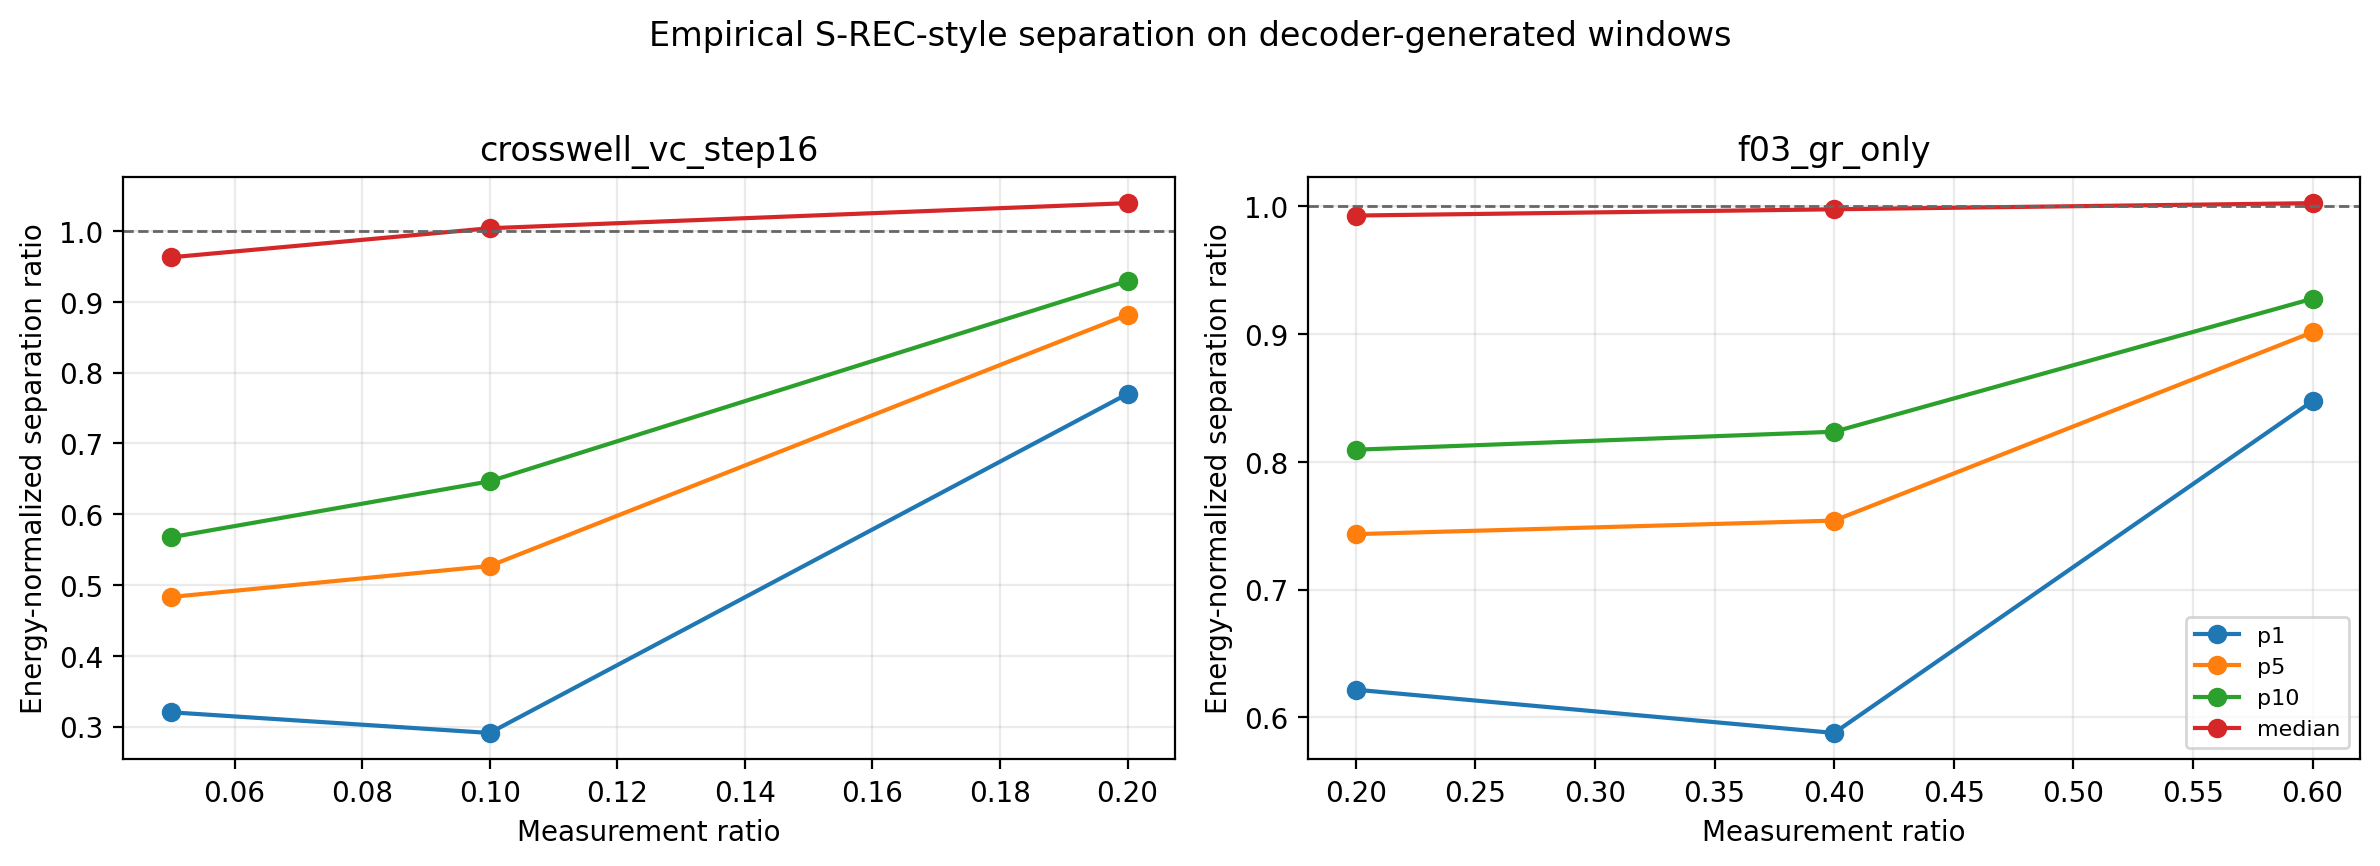
\includegraphics[width=\linewidth]{srec_percentiles.png}
  \caption{Empirical S-REC-style separation diagnostics. The curves show lower
  percentiles and medians of the energy-normalized pairwise separation ratio on
  decoder-generated windows returned to the original target units. Higher lower-percentile values indicate stronger
  separation of plausible generated candidates under coordinate subsampling.}
  \label{fig:srec_percentiles}
\end{figure}

\subsection{Full F03-4 benchmark table}
\label{app:f03_full_table}

Table~\ref{tab:f03_results_full} reports the complete single-well F03-4 GR-only
porosity benchmark used in Section~\ref{subsec:f03_gr_only_results}. In addition
to mean RMSE, it includes seed-level RMSE variability (standard deviation and
Student-$t$ $95\%$ half-width with $\mathrm{df}=2$), MAE, and relative
$\ell_2$ error for all seven methods at each tested measurement ratio.

\begin{table}[htbp]
  \centering
  \caption{Full single-well F03-4 GR-only porosity benchmark by measurement ratio,
  including direct baselines, structural reference variants, and multi-metric
  summaries across seeds. The column $\mathrm{rmse\_t95\_half}$ is the
  Student-$t$ $95\%$ half-width for the seed mean ($\mathrm{df}=2$), not a
  normal $z=1.96$ interval.}
  \label{tab:f03_results_full}
  \small
  \adjustbox{max width=\linewidth}{\begin{tabular}{rlrrrrr}
\toprule
rho & method & rmse & rmse\_std & rmse\_t95\_half & mae & relative\_l2 \\
\midrule
0.20000 & CLP-CSGM Ridge & 0.01596 & 0.00010 & 0.00024 & 0.01409 & 0.06000 \\
0.20000 & AE [u,b] & 0.01850 & 0.00067 & 0.00166 & 0.01619 & 0.06951 \\
0.20000 & Prior-only Ridge & 0.01958 & 0.00009 & 0.00022 & 0.01774 & 0.07360 \\
0.20000 & PCA [u,b] & 0.02149 & 0.00093 & 0.00230 & 0.01796 & 0.08073 \\
0.20000 & ML only & 0.02359 & 0.00051 & 0.00126 & 0.02086 & 0.08866 \\
0.20000 & Measurement-only CSGM & 0.02519 & 0.00145 & 0.00360 & 0.01993 & 0.09459 \\
0.20000 & MLP [u,b] & 0.03022 & 0.00059 & 0.00146 & 0.02588 & 0.11356 \\
0.30000 & CLP-CSGM Ridge & 0.01475 & 0.00067 & 0.00166 & 0.01294 & 0.05544 \\
0.30000 & AE [u,b] & 0.01554 & 0.00011 & 0.00027 & 0.01351 & 0.05837 \\
0.30000 & Prior-only Ridge & 0.01958 & 0.00009 & 0.00022 & 0.01774 & 0.07360 \\
0.30000 & PCA [u,b] & 0.02187 & 0.00130 & 0.00323 & 0.01799 & 0.08214 \\
0.30000 & Measurement-only CSGM & 0.02285 & 0.00117 & 0.00290 & 0.01786 & 0.08578 \\
0.30000 & ML only & 0.02359 & 0.00051 & 0.00126 & 0.02086 & 0.08866 \\
0.30000 & MLP [u,b] & 0.02997 & 0.00270 & 0.00670 & 0.02555 & 0.11253 \\
0.40000 & AE [u,b] & 0.01304 & 0.00013 & 0.00033 & 0.01116 & 0.04897 \\
0.40000 & CLP-CSGM Ridge & 0.01377 & 0.00052 & 0.00129 & 0.01197 & 0.05176 \\
0.40000 & Prior-only Ridge & 0.01958 & 0.00009 & 0.00022 & 0.01774 & 0.07360 \\
0.40000 & Measurement-only CSGM & 0.02033 & 0.00182 & 0.00452 & 0.01560 & 0.07635 \\
0.40000 & PCA [u,b] & 0.02261 & 0.00172 & 0.00427 & 0.01839 & 0.08490 \\
0.40000 & ML only & 0.02359 & 0.00051 & 0.00126 & 0.02086 & 0.08866 \\
0.40000 & MLP [u,b] & 0.03712 & 0.00166 & 0.00412 & 0.03244 & 0.13932 \\
0.50000 & CLP-CSGM Ridge & 0.01281 & 0.00048 & 0.00119 & 0.01110 & 0.04813 \\
0.50000 & AE [u,b] & 0.01286 & 0.00010 & 0.00025 & 0.01107 & 0.04832 \\
0.50000 & Measurement-only CSGM & 0.01622 & 0.00087 & 0.00217 & 0.01281 & 0.06089 \\
0.50000 & Prior-only Ridge & 0.01958 & 0.00009 & 0.00022 & 0.01774 & 0.07360 \\
0.50000 & ML only & 0.02359 & 0.00051 & 0.00126 & 0.02086 & 0.08866 \\
0.50000 & PCA [u,b] & 0.02409 & 0.00301 & 0.00748 & 0.01952 & 0.09050 \\
0.50000 & MLP [u,b] & 0.04199 & 0.00227 & 0.00564 & 0.03757 & 0.15764 \\
0.60000 & AE [u,b] & 0.01178 & 0.00023 & 0.00058 & 0.01003 & 0.04425 \\
0.60000 & CLP-CSGM Ridge & 0.01220 & 0.00041 & 0.00102 & 0.01051 & 0.04583 \\
0.60000 & Measurement-only CSGM & 0.01494 & 0.00081 & 0.00200 & 0.01176 & 0.05611 \\
0.60000 & Prior-only Ridge & 0.01958 & 0.00009 & 0.00022 & 0.01774 & 0.07360 \\
0.60000 & ML only & 0.02359 & 0.00051 & 0.00126 & 0.02086 & 0.08866 \\
0.60000 & PCA [u,b] & 0.02426 & 0.00114 & 0.00284 & 0.01976 & 0.09109 \\
0.60000 & MLP [u,b] & 0.04627 & 0.00483 & 0.01199 & 0.04076 & 0.17381 \\
\bottomrule
\end{tabular}
}
\end{table}

\subsection{F03-4 Metric Robustness Views}
\label{app:f03_metric_views}

The F03-4 GR-only discussion in Section~\ref{subsec:f03_gr_only_results} uses
RMSE because the protocol selects and reports models on that scale.
Figures~\ref{fig:f03_mae} and~\ref{fig:f03_rell2} evaluate the same
interpretation under alternative error summaries. MAE downweights isolated large
deviations relative to RMSE. Relative \(\ell_2\) error indicates whether the
ranking mainly reflects a scale effect. Both plots retain the sparse-regime
pattern: CLP-CSGM Ridge is lowest or close to lowest at lower measurement
ratios, and AE \([u,b]\) becomes more competitive as more entries of \(b\) are
available.
The degradation of direct MLP \([u,b]\) also appears in more than one metric,
consistent with sparse measurements acting as high-variance features when the
measurement operator is not handled explicitly.

\begin{figure}[htbp]
  \centering
  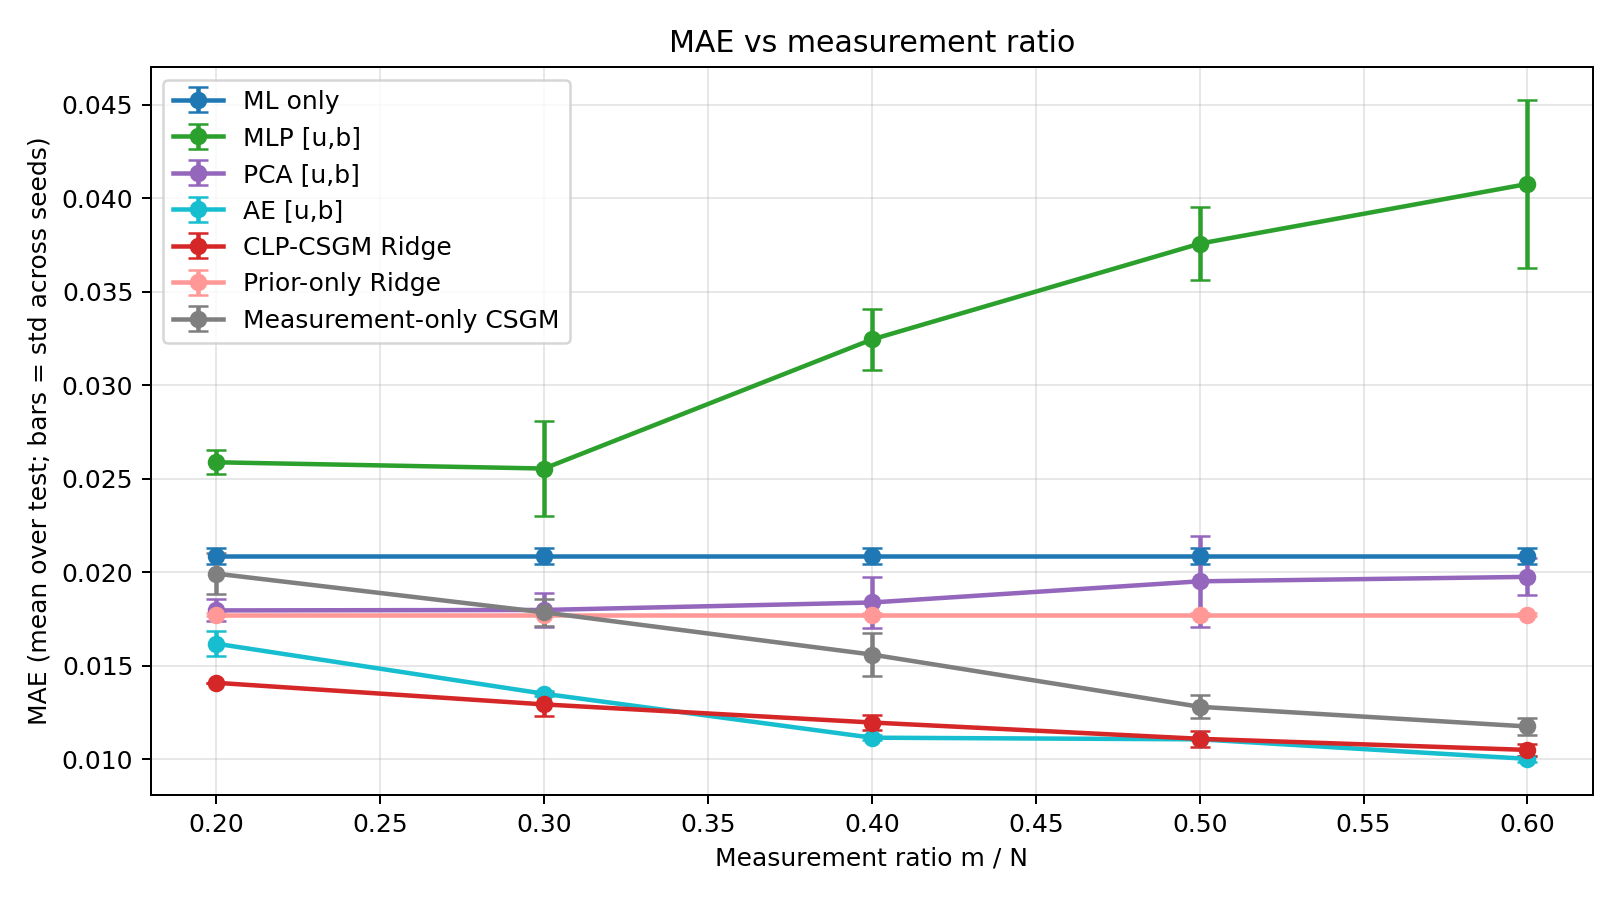
\includegraphics[width=0.92\linewidth]{figures/02_mae_vs_measurement_ratio.png}
  \caption{Single-well F03-4 GR-only MAE by measurement ratio. The ranking is
  consistent with the RMSE view in the main text: CLP-CSGM Ridge has the lowest
  MAE in the sparse regime and remains competitive as the measurement ratio
  increases.}
  \label{fig:f03_mae}
\end{figure}

\begin{figure}[htbp]
  \centering
  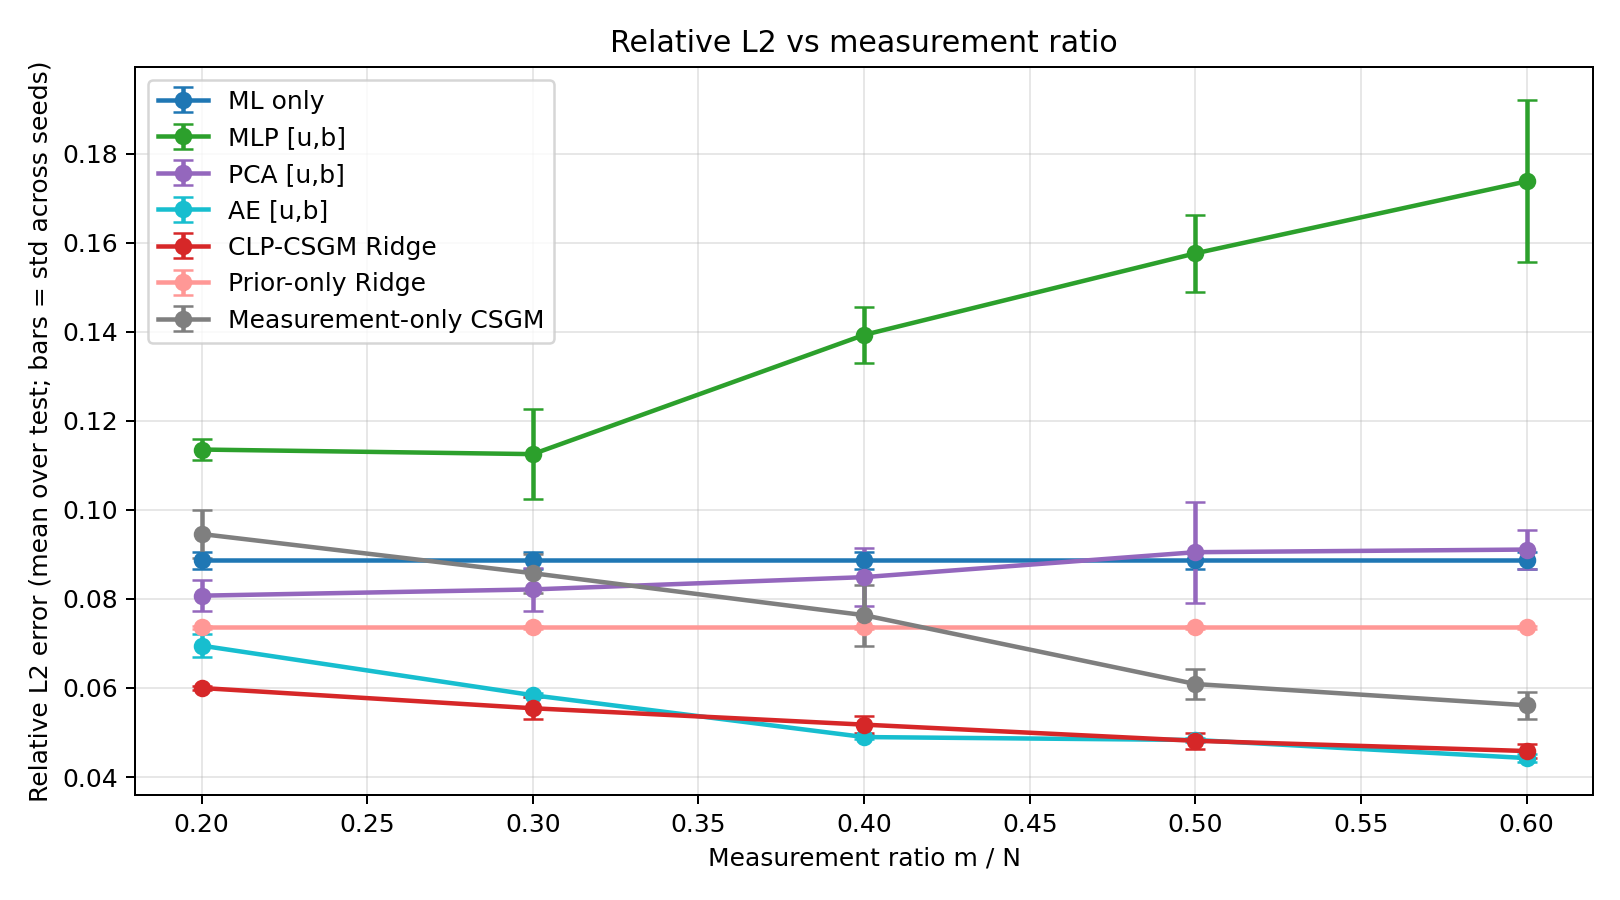
\includegraphics[width=0.92\linewidth]{figures/03_relative_l2_vs_measurement_ratio.png}
  \caption{Relative \(\ell_2\) error on the single-well F03-4 GR-only benchmark.
  The relative-error view preserves the same conclusion as RMSE and MAE,
  indicating that the gain is not caused by scale effects alone.}
  \label{fig:f03_rell2}
\end{figure}

\subsection{Illustrative sparse-measurement windows}
\label{app:sparse_recon_examples}

The main tables and curves in Section~\ref{sec:results} pool scalar errors over
many test windows. The examples in
Figs.~\ref{fig:sparse_recon_f03} and~\ref{fig:sparse_recon_crosswell} display the
target profile, the coordinates where \(b\) is observed, and the full-window
predictions generated under the paired \((\text{seed},\rho)\) design used in the
main experiments, thereby complementing the aggregate comparisons with
window-level views.

The horizontal axis indexes coordinates within one length-\(L\) window
(\(L=64\)). The blue curve is the target window \(y\). Black markers show the
realized noisy measurements \(b\) at the sampled coordinates. The red curve is
CLP-CSGM Ridge and the green curve is AE \([u,b]\), when shown. These markers
are the actual sparse inputs generated under the benchmark noise model.

Each figure fixes one test-window index, one seed, and one \(\rho\). These audit
examples show that the markers alone underdetermine the reconstruction and that
the methods interpolate between sparse constraints using different inductive
biases. In the displayed porosity window, both CLP-CSGM Ridge and AE \([u,b]\)
miss the central depression of the reference. In the displayed clay-volume
window, the corresponding configuration is step 16, seed 7, \(\rho=0.10\), and
window index 0. CLP-CSGM Ridge is closer to the reference, the autoencoder
prediction is positively offset, and local deviations remain. These windows do
not establish a uniform advantage. Aggregate tables and the main-text
diagnostics provide the overall performance comparisons.

\begin{figure}[htbp]
  \centering
  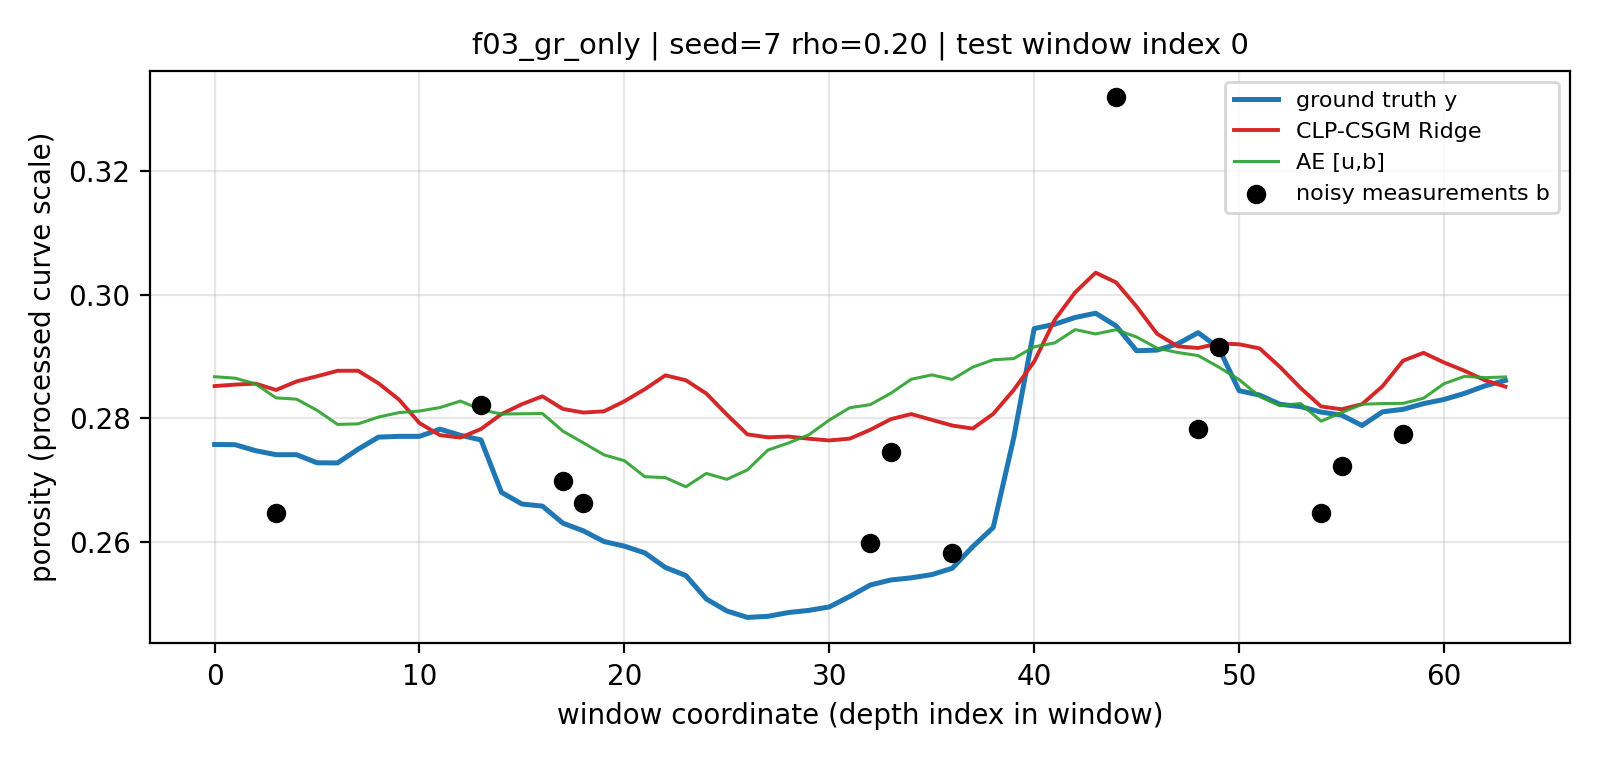
\includegraphics[width=\linewidth]{figures/f03_gr_only_seed7_rho0p2_ex0.png}
  \caption{F03-4 GR-only porosity example (test window index 0, seed 7, \(\rho=0.20\)):
  ground truth, sparse noisy measurements \(b\), CLP-CSGM Ridge, and AE \([u,b]\).
  In this displayed window, both reconstructions miss the central depression of
  the reference.}
  \label{fig:sparse_recon_f03}
\end{figure}

\begin{figure}[htbp]
  \centering
  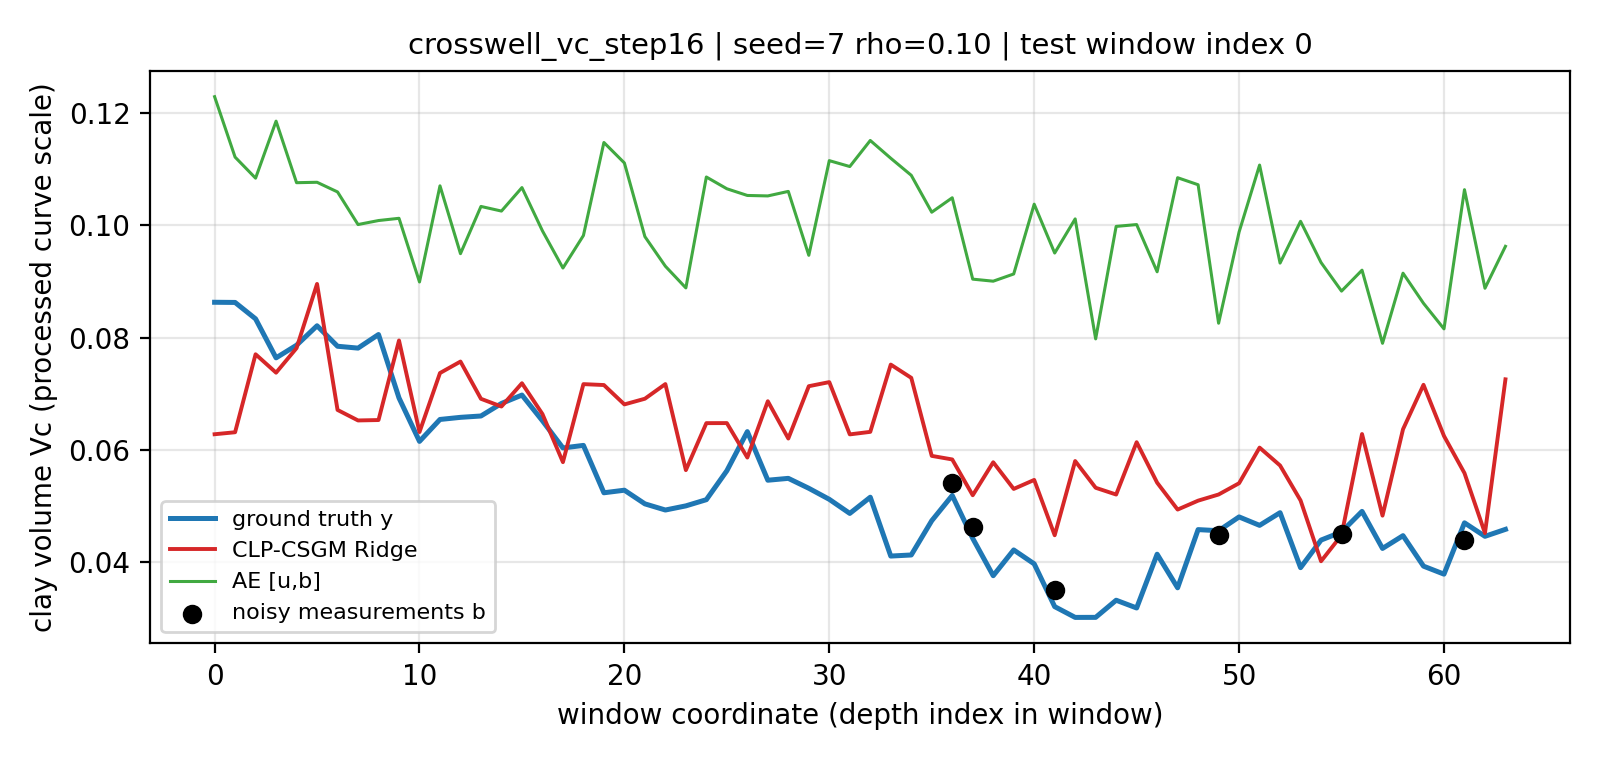
\includegraphics[width=\linewidth]{figures/crosswell_vc_step16_seed7_rho0p1_ex0.png}
  \caption{Cross-well \(V_c\) example (held-out F03-4 test window index 0, step 16, seed 7,
  \(\rho=0.10\)): ground truth, sparse noisy measurements \(b\), CLP-CSGM Ridge, and AE \([u,b]\).
  In this displayed window, CLP-CSGM Ridge is closer to the reference. The
  autoencoder prediction is positively offset, and local deviations remain.}
  \label{fig:sparse_recon_crosswell}
\end{figure}

\subsection{F03-4 Qualitative Reconstruction Views}
\label{app:f03_qualitative_views}

This subsection complements the depth-profile reconstruction in the main text
(Fig.~\ref{fig:f03_depth}). Because the depth profile follows the contiguous test
interval, it provides the clearest qualitative view. The figures below present
window-level and pointwise audits.

Figure~\ref{fig:f03_examples} shows representative F03-4 test windows and reveals
local shape behavior compressed by scalar metrics. Direct MLP \([u,b]\) can
produce oscillatory predictions, whereas PCA, AE, and CLP-CSGM Ridge are
smoother. In these displayed windows, CLP-CSGM Ridge and the autoencoder miss
part of the central depression of the reference. Aggregate metrics determine
the window-level rankings.
Figure~\ref{fig:f03_parity} pools pointwise predictions against ground
truth over the F03-4 test windows. The figure prints a correlation of
$0.4632$ for CLP-CSGM Ridge and $0.3720$ for AE \([u,b]\). The scatter remains
broad. This comparison describes the pooled points on the plot. It does not
establish statistical significance, and overlapping-window predictions are not
independent observations.

\begin{figure}[htbp]
  \centering
  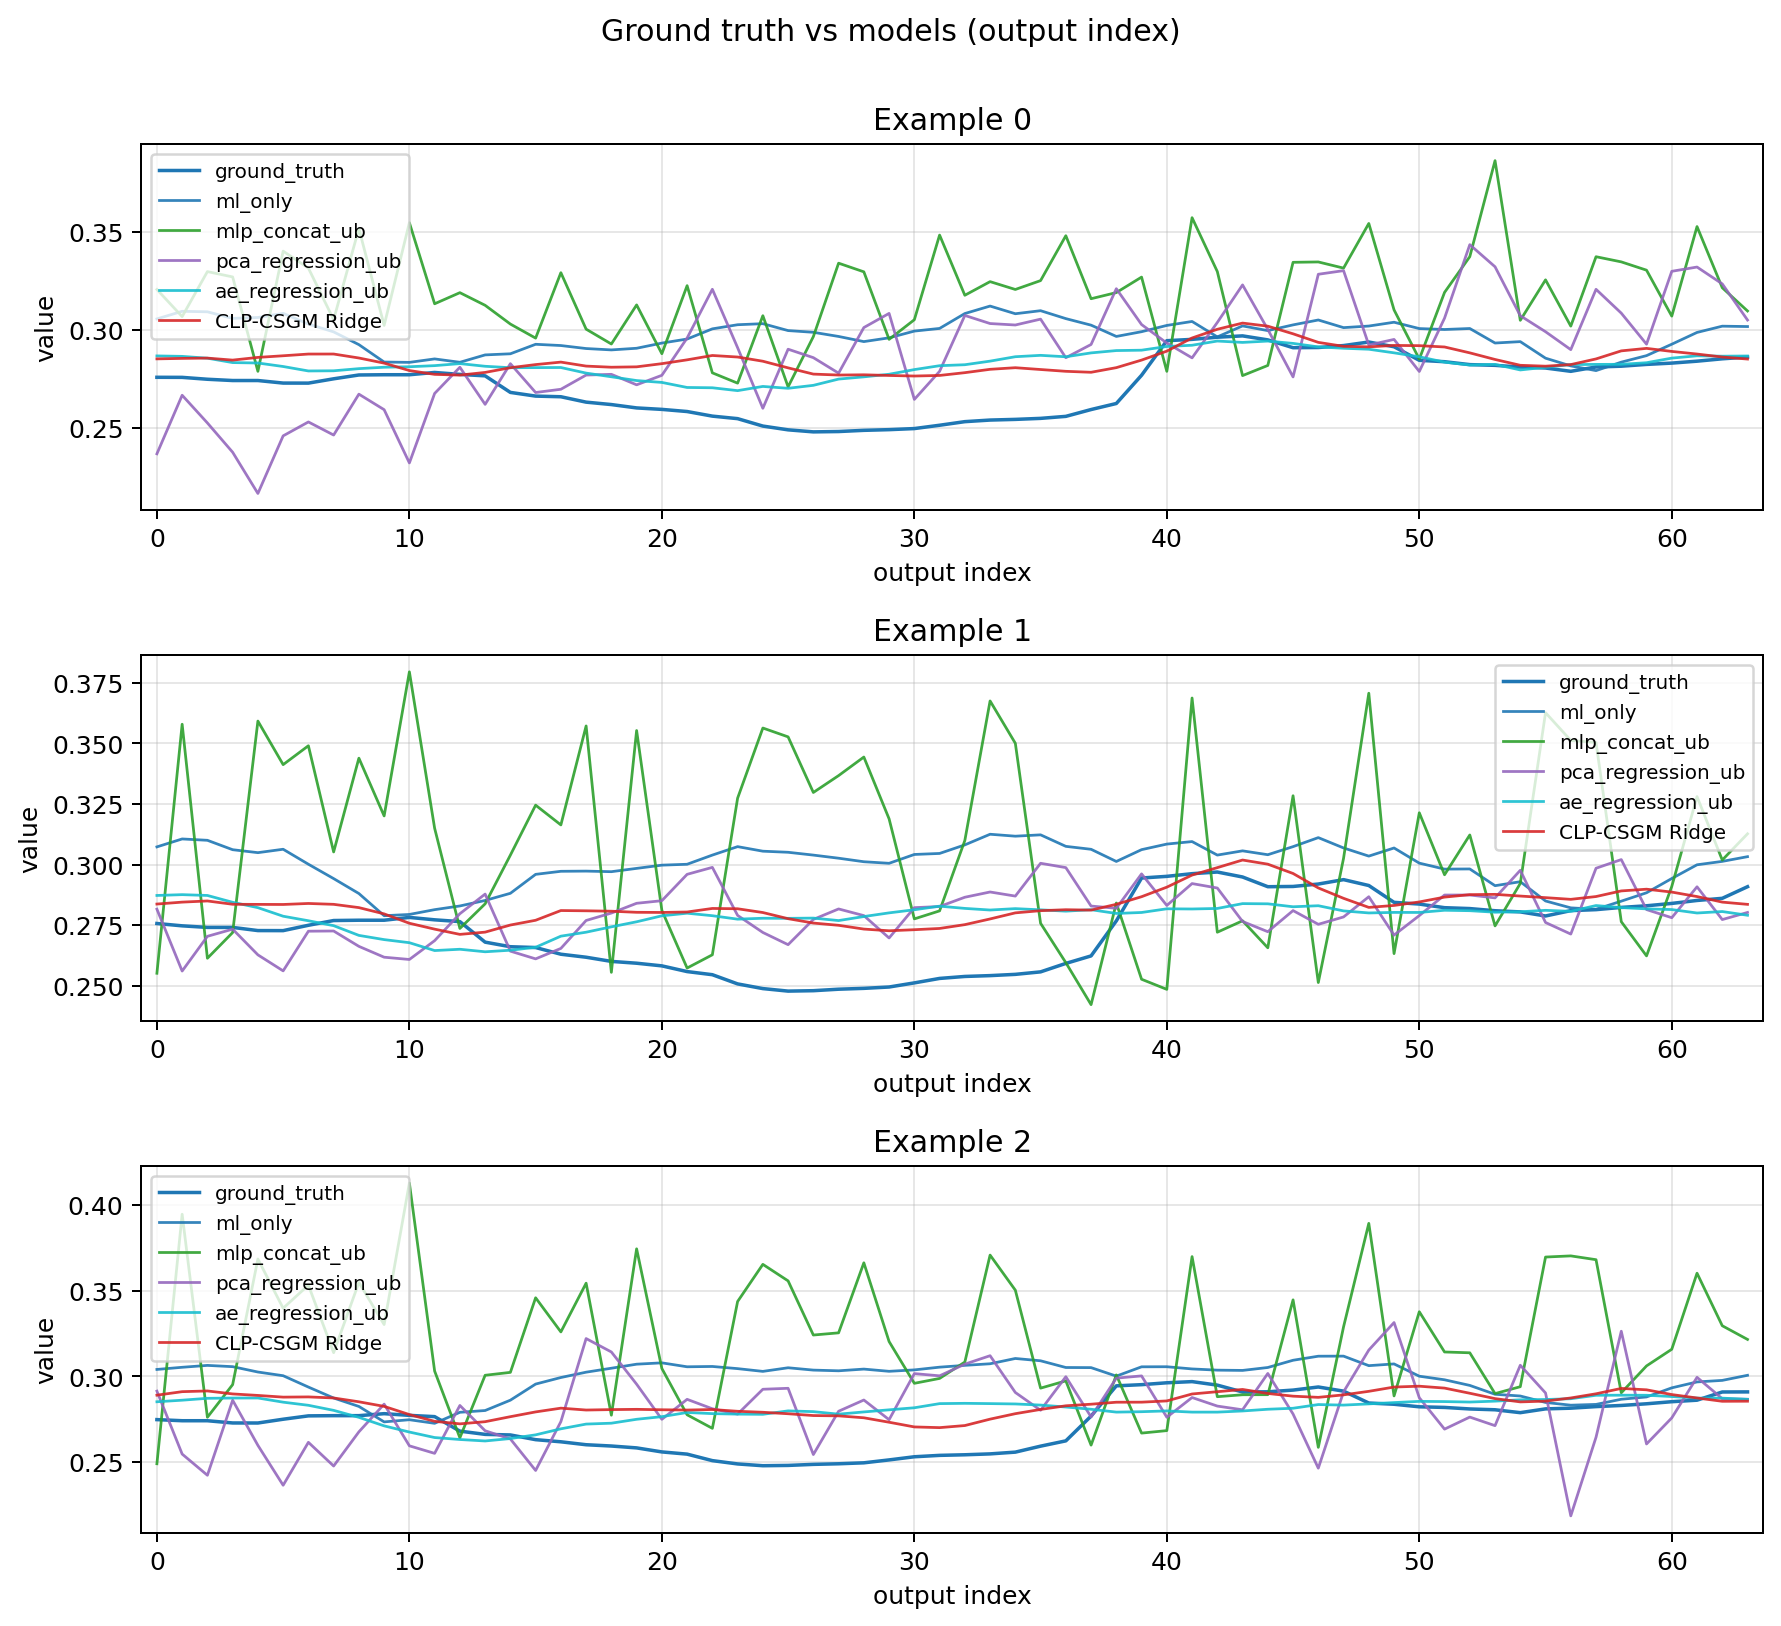
\includegraphics[width=\linewidth]{figures/08_example_ground_truth_vs_models.png}
  \caption{Representative F03-4 test windows. Direct MLP \([u,b]\) is visibly
  more oscillatory. CLP-CSGM Ridge and AE \([u,b]\) are smoother and, in these
  displayed windows, miss part of the central depression of the reference.}
  \label{fig:f03_examples}
\end{figure}

\begin{figure}[htbp]
  \centering
  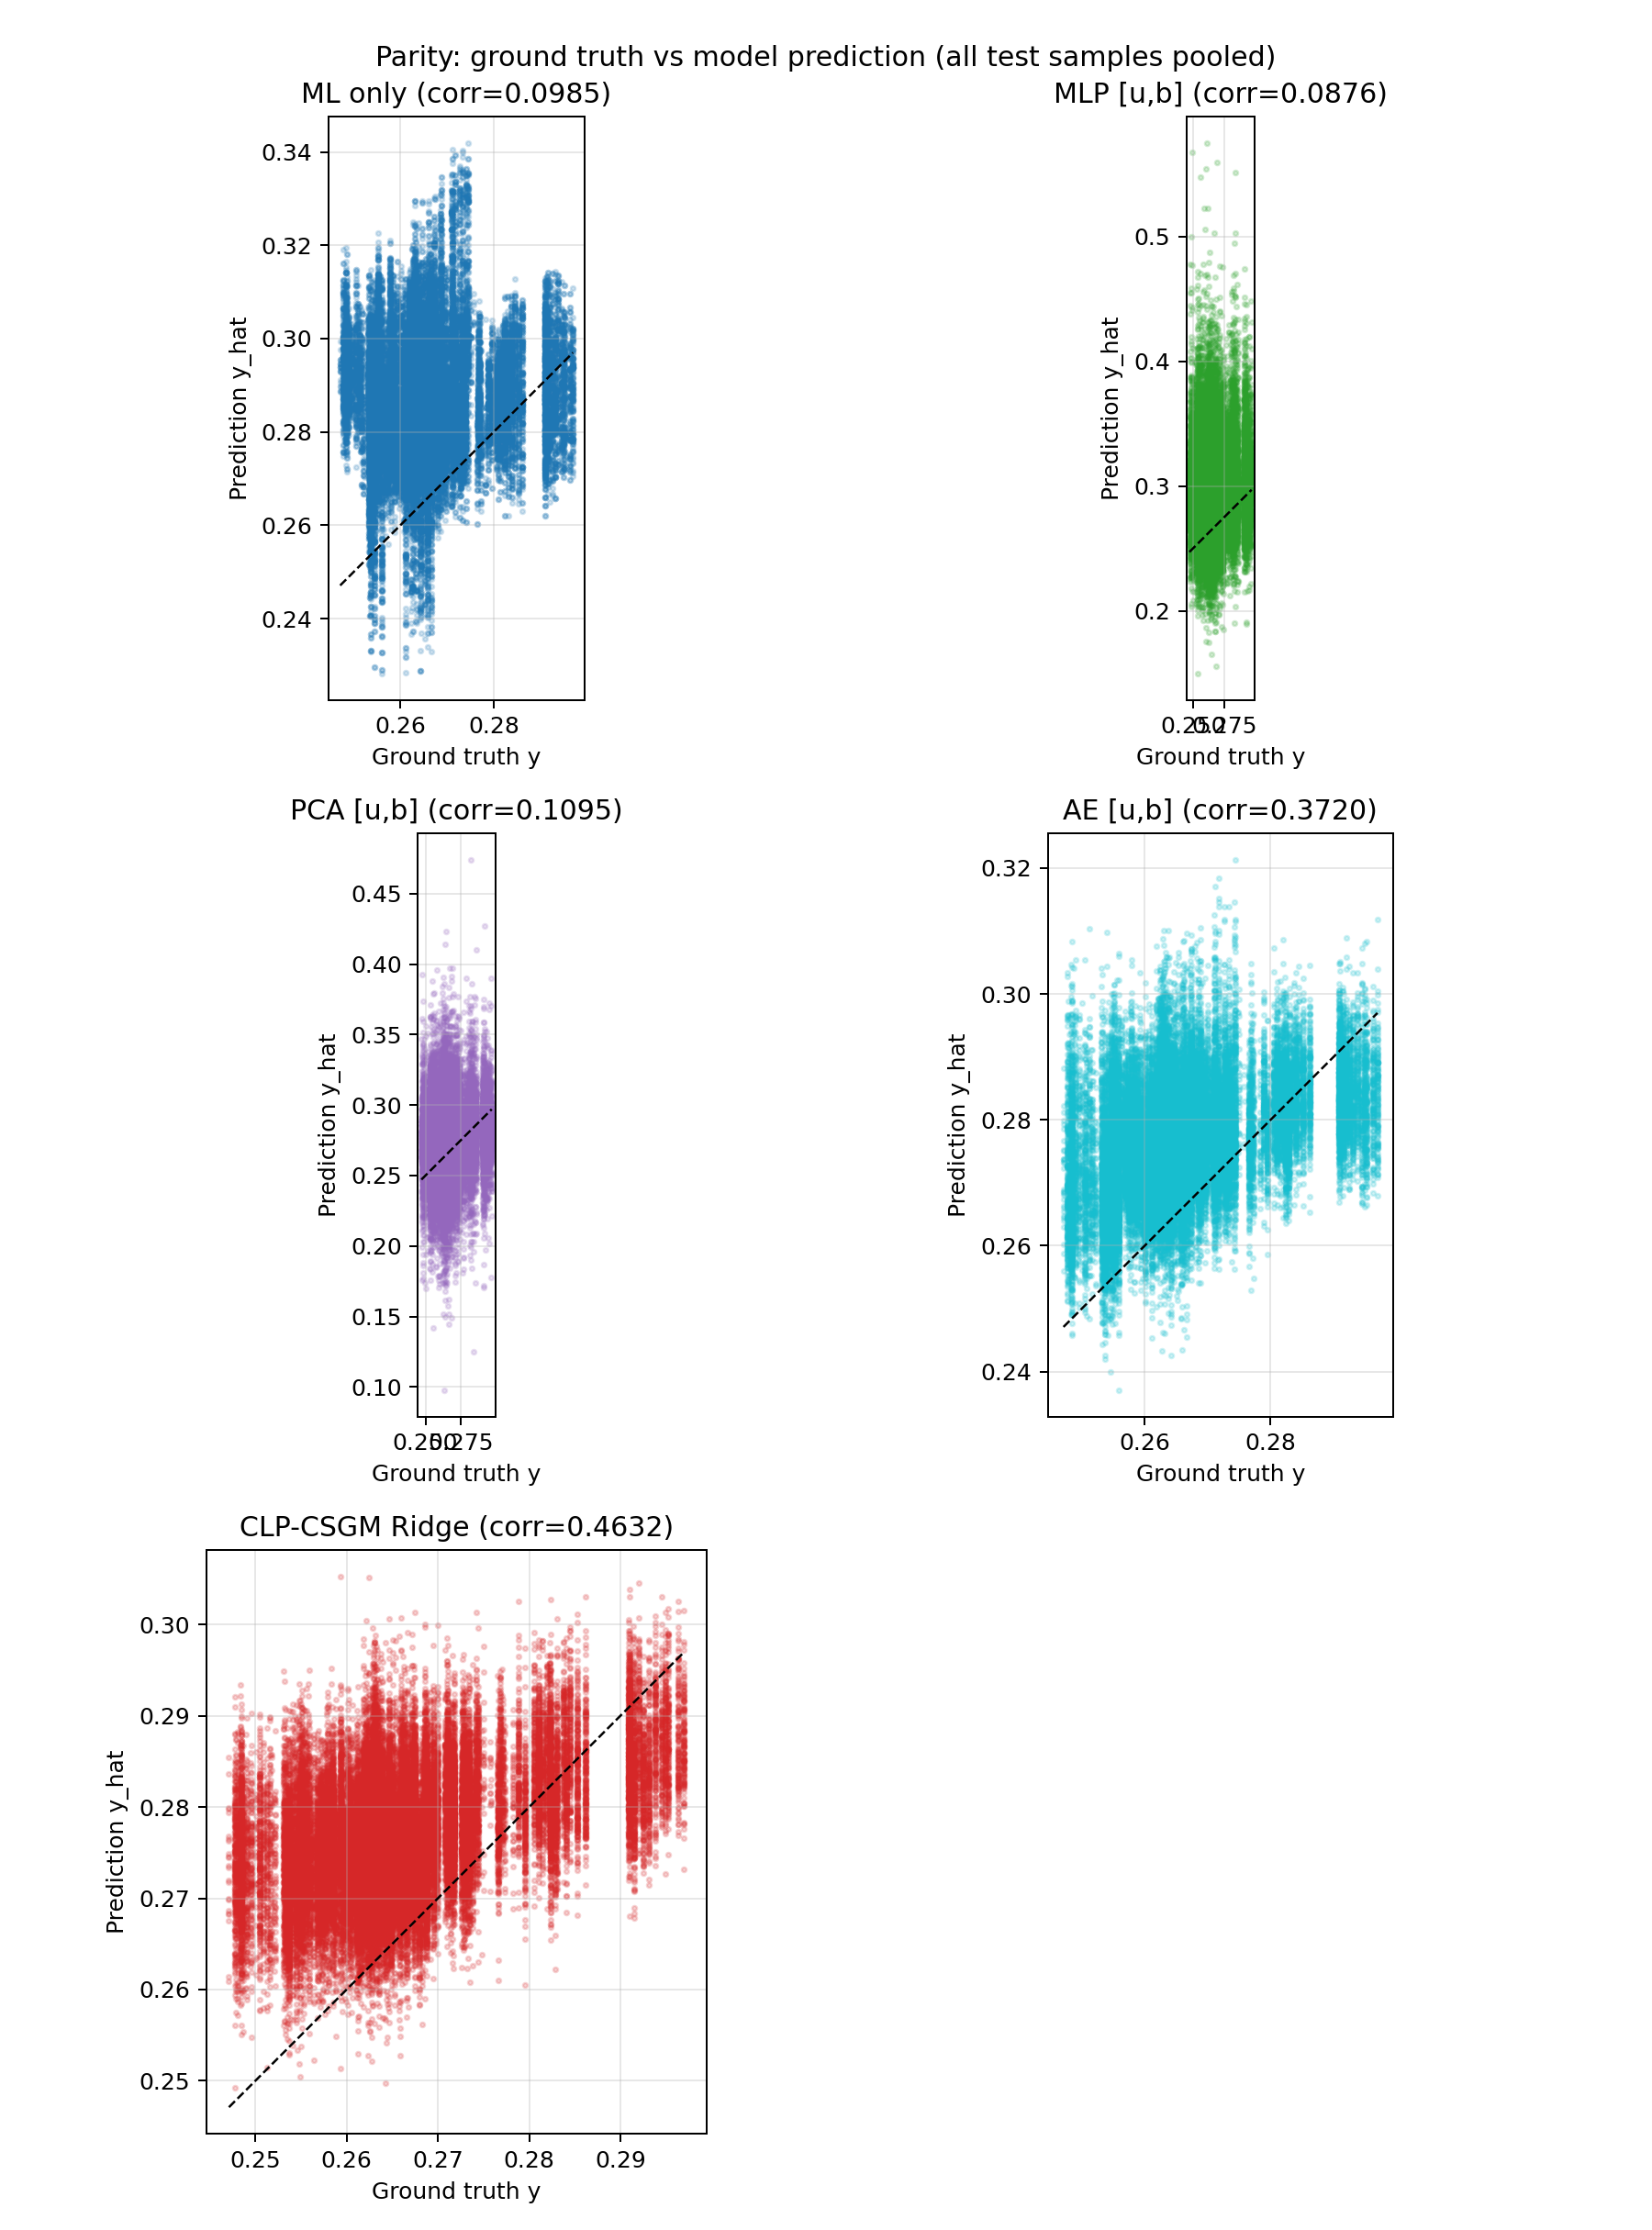
\includegraphics[width=0.82\linewidth]{figures/09_parity_ground_truth_vs_prediction.png}
  \caption{Pooled parity plots for F03-4 test windows. The displayed correlations
  are $0.4632$ for CLP-CSGM Ridge and $0.3720$ for AE \([u,b]\). Broad scatter
  remains. These values describe the pooled points on the figure and are not a
  significance test.}
  \label{fig:f03_parity}
\end{figure}

\subsection{Validation and Generalization Diagnostics}
\label{app:validation_generalization_diagnostics}

Figures~\ref{fig:diagnostic_crosswell} and~\ref{fig:diagnostic_f03} audit
quantities used by the experimental protocol: validation RMSE for selecting
\(\lambda\), selected regularization values, per-window test RMSE distributions,
and the relation between autoencoder training reconstruction error and final test
RMSE. These diagnostics support the reliability and interpretation of the main
rankings.

Figure~\ref{fig:diagnostic_crosswell} summarizes the cross-well \(V_c\) case.
The validation and test RMSE values remain of similar magnitude across the
low-data grid, with no sign that lower validation error is obtained only by
shifting error to the test well. The selected \(\lambda\) values are small but
nonzero, consistent with sparse target-log observations providing the main
target-well information while the log-conditioned latent prior acts as a
stabilizing regularizer. The per-window RMSE boxplots reinforce the ablation
result: CLP-CSGM Ridge has a lower median error than the latent-prior-only
decoder and a substantially tighter distribution than measurement-only CSGM.

\begin{figure}[htbp]
  \centering
  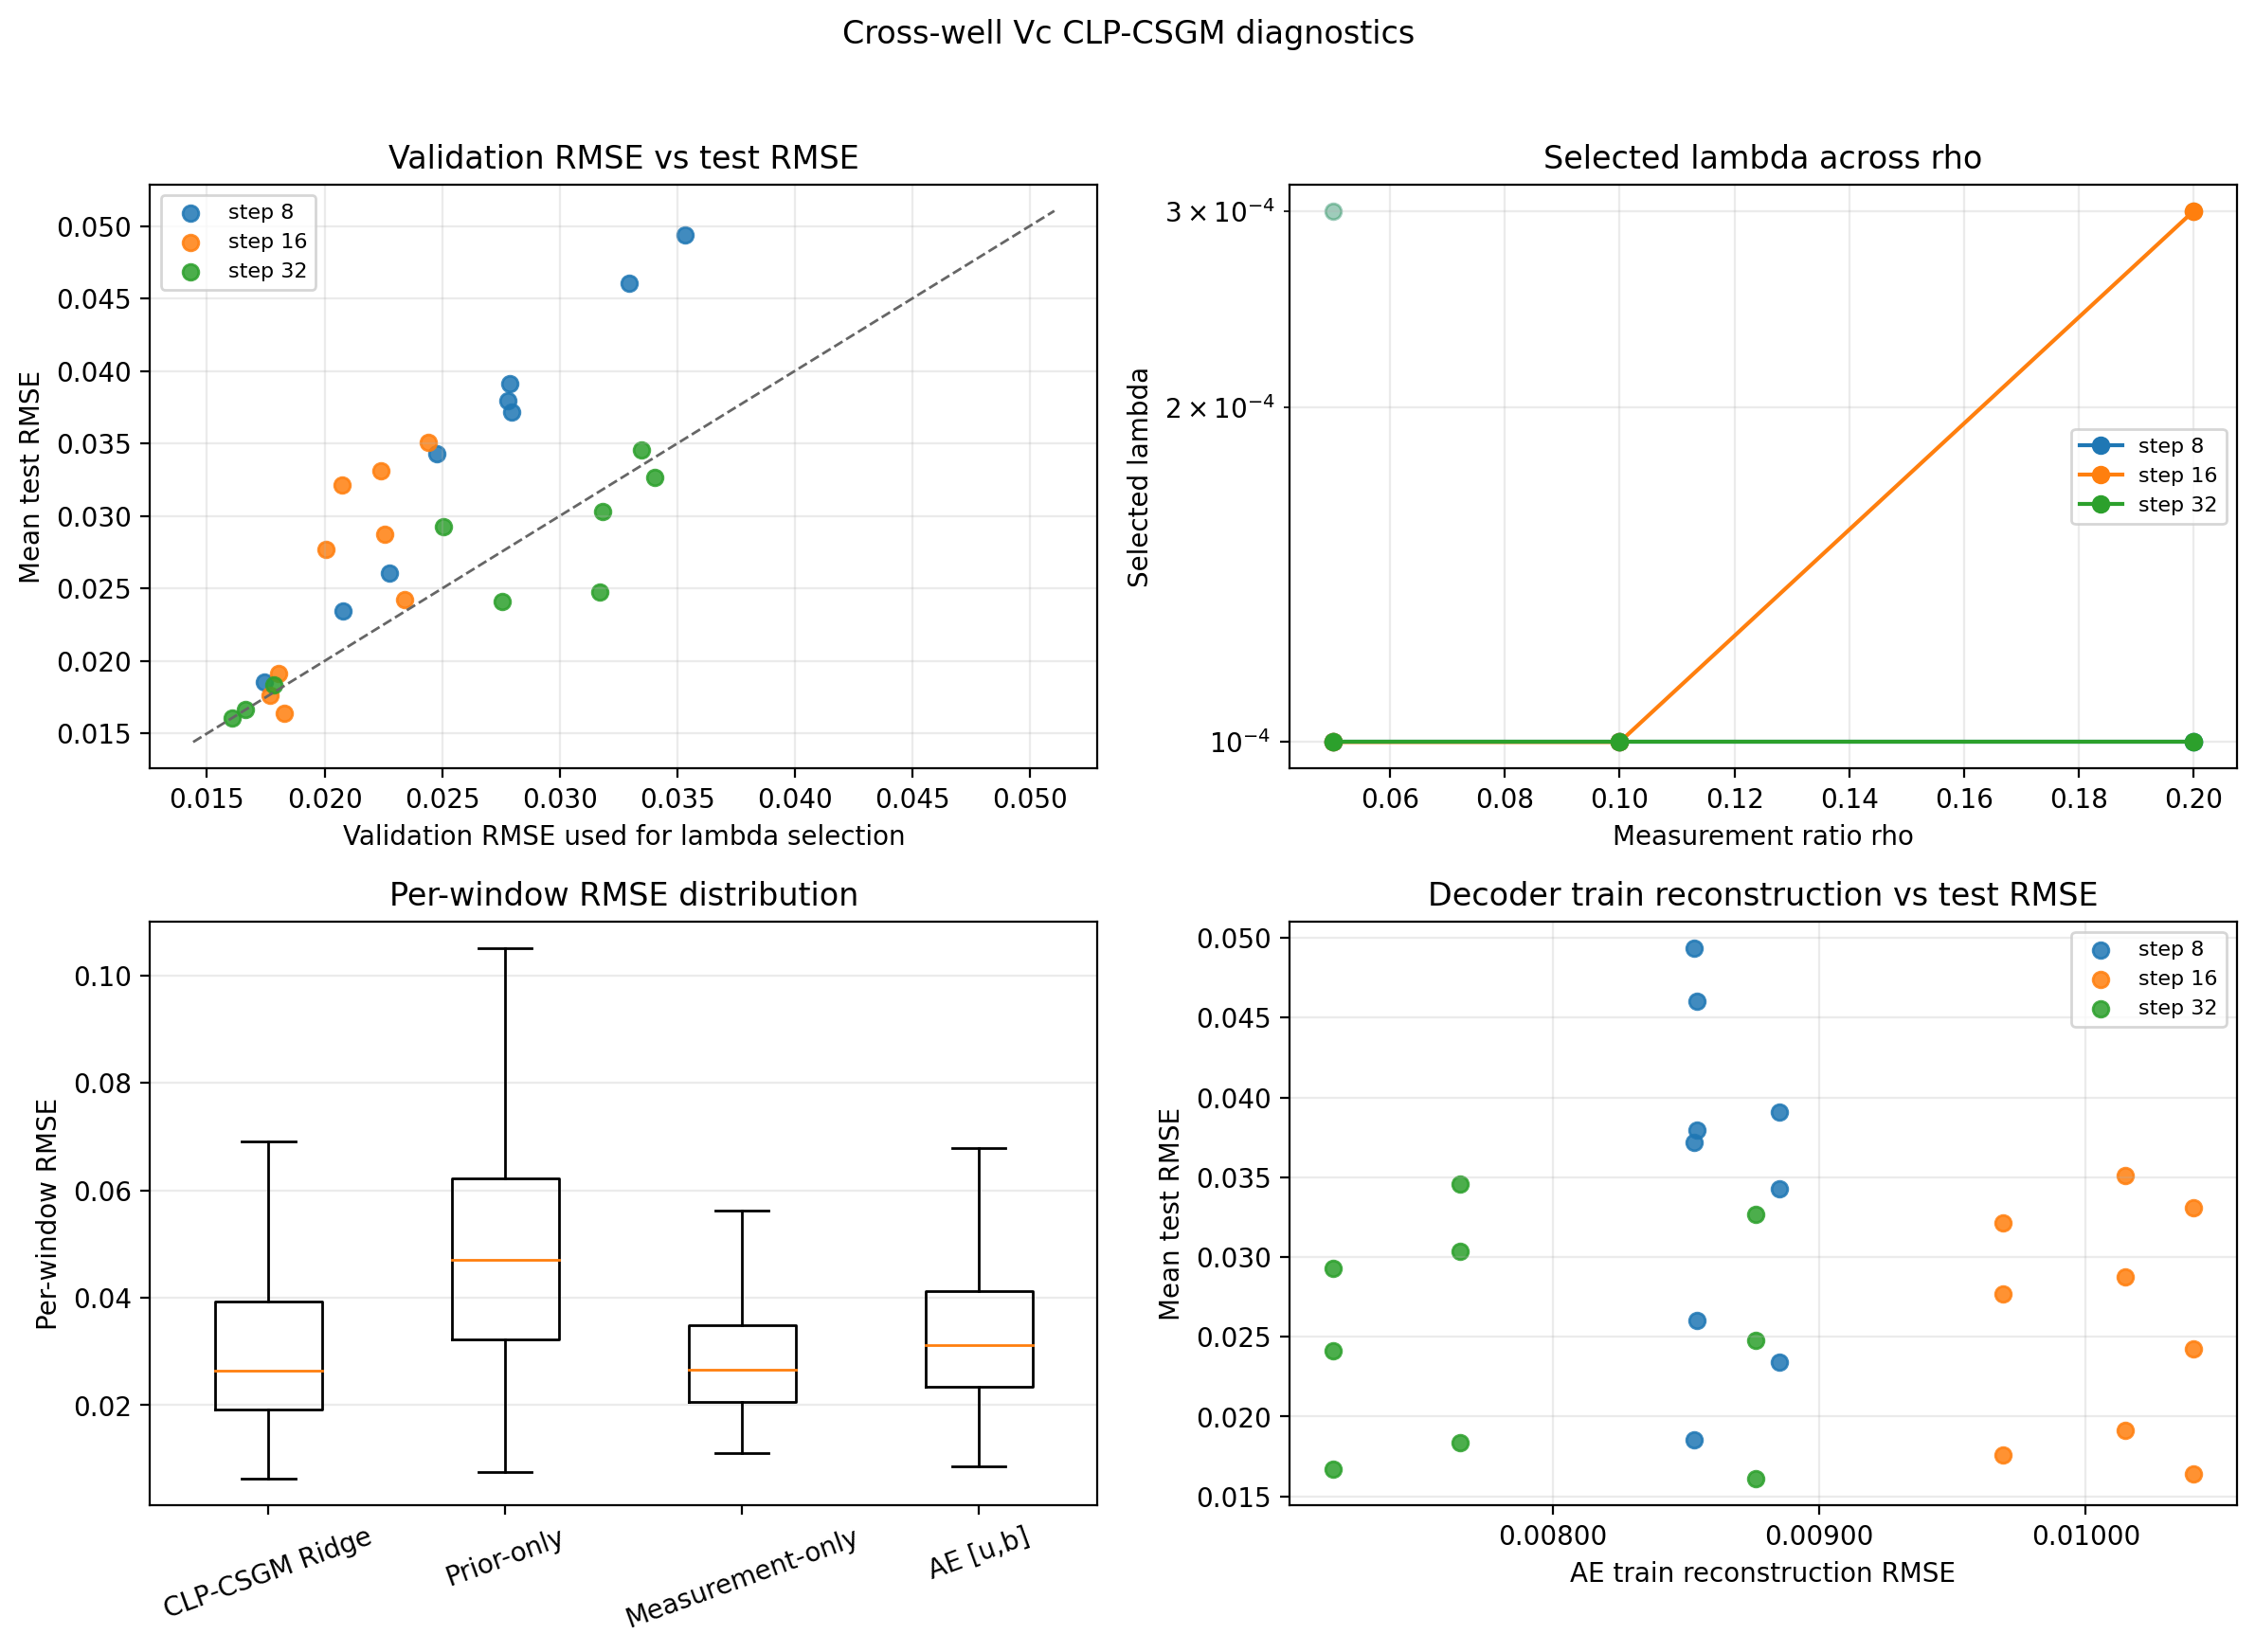
\includegraphics[width=\linewidth]{figures/diagnostic_crosswell_generalization.png}
  \caption{Cross-well \(V_c\) diagnostics for CLP-CSGM Ridge summarizing the experiments in Section~\ref{subsec:crosswell_results}. The
  panels compare validation RMSE with mean test RMSE for CLP-CSGM Ridge, show the
  selected \(\lambda\) values across measurement ratios, summarize per-window
  RMSE distributions, and relate autoencoder training reconstruction error to
  final test RMSE.}
  \label{fig:diagnostic_crosswell}
\end{figure}

Figure~\ref{fig:diagnostic_f03} gives the analogous diagnostic view for the
F03-4 porosity benchmark with GR-only dense input. The validation--test relation
is less diagonal than in the cross-well case, consistent with the harder stress
test: the dense input is restricted to GR, and the test block is a contiguous
depth interval, not a random split. The trend across measurement ratios remains
coherent. Larger \(\rho\) generally reduces the full-model test
error, and the selected \(\lambda\) remains stable across ratios. The
per-window RMSE distributions show that CLP-CSGM Ridge improves the central
error relative to both ablated variants while remaining close to AE \([u,b]\),
matching the main F03 regime-dependent result.

\begin{figure}[htbp]
  \centering
  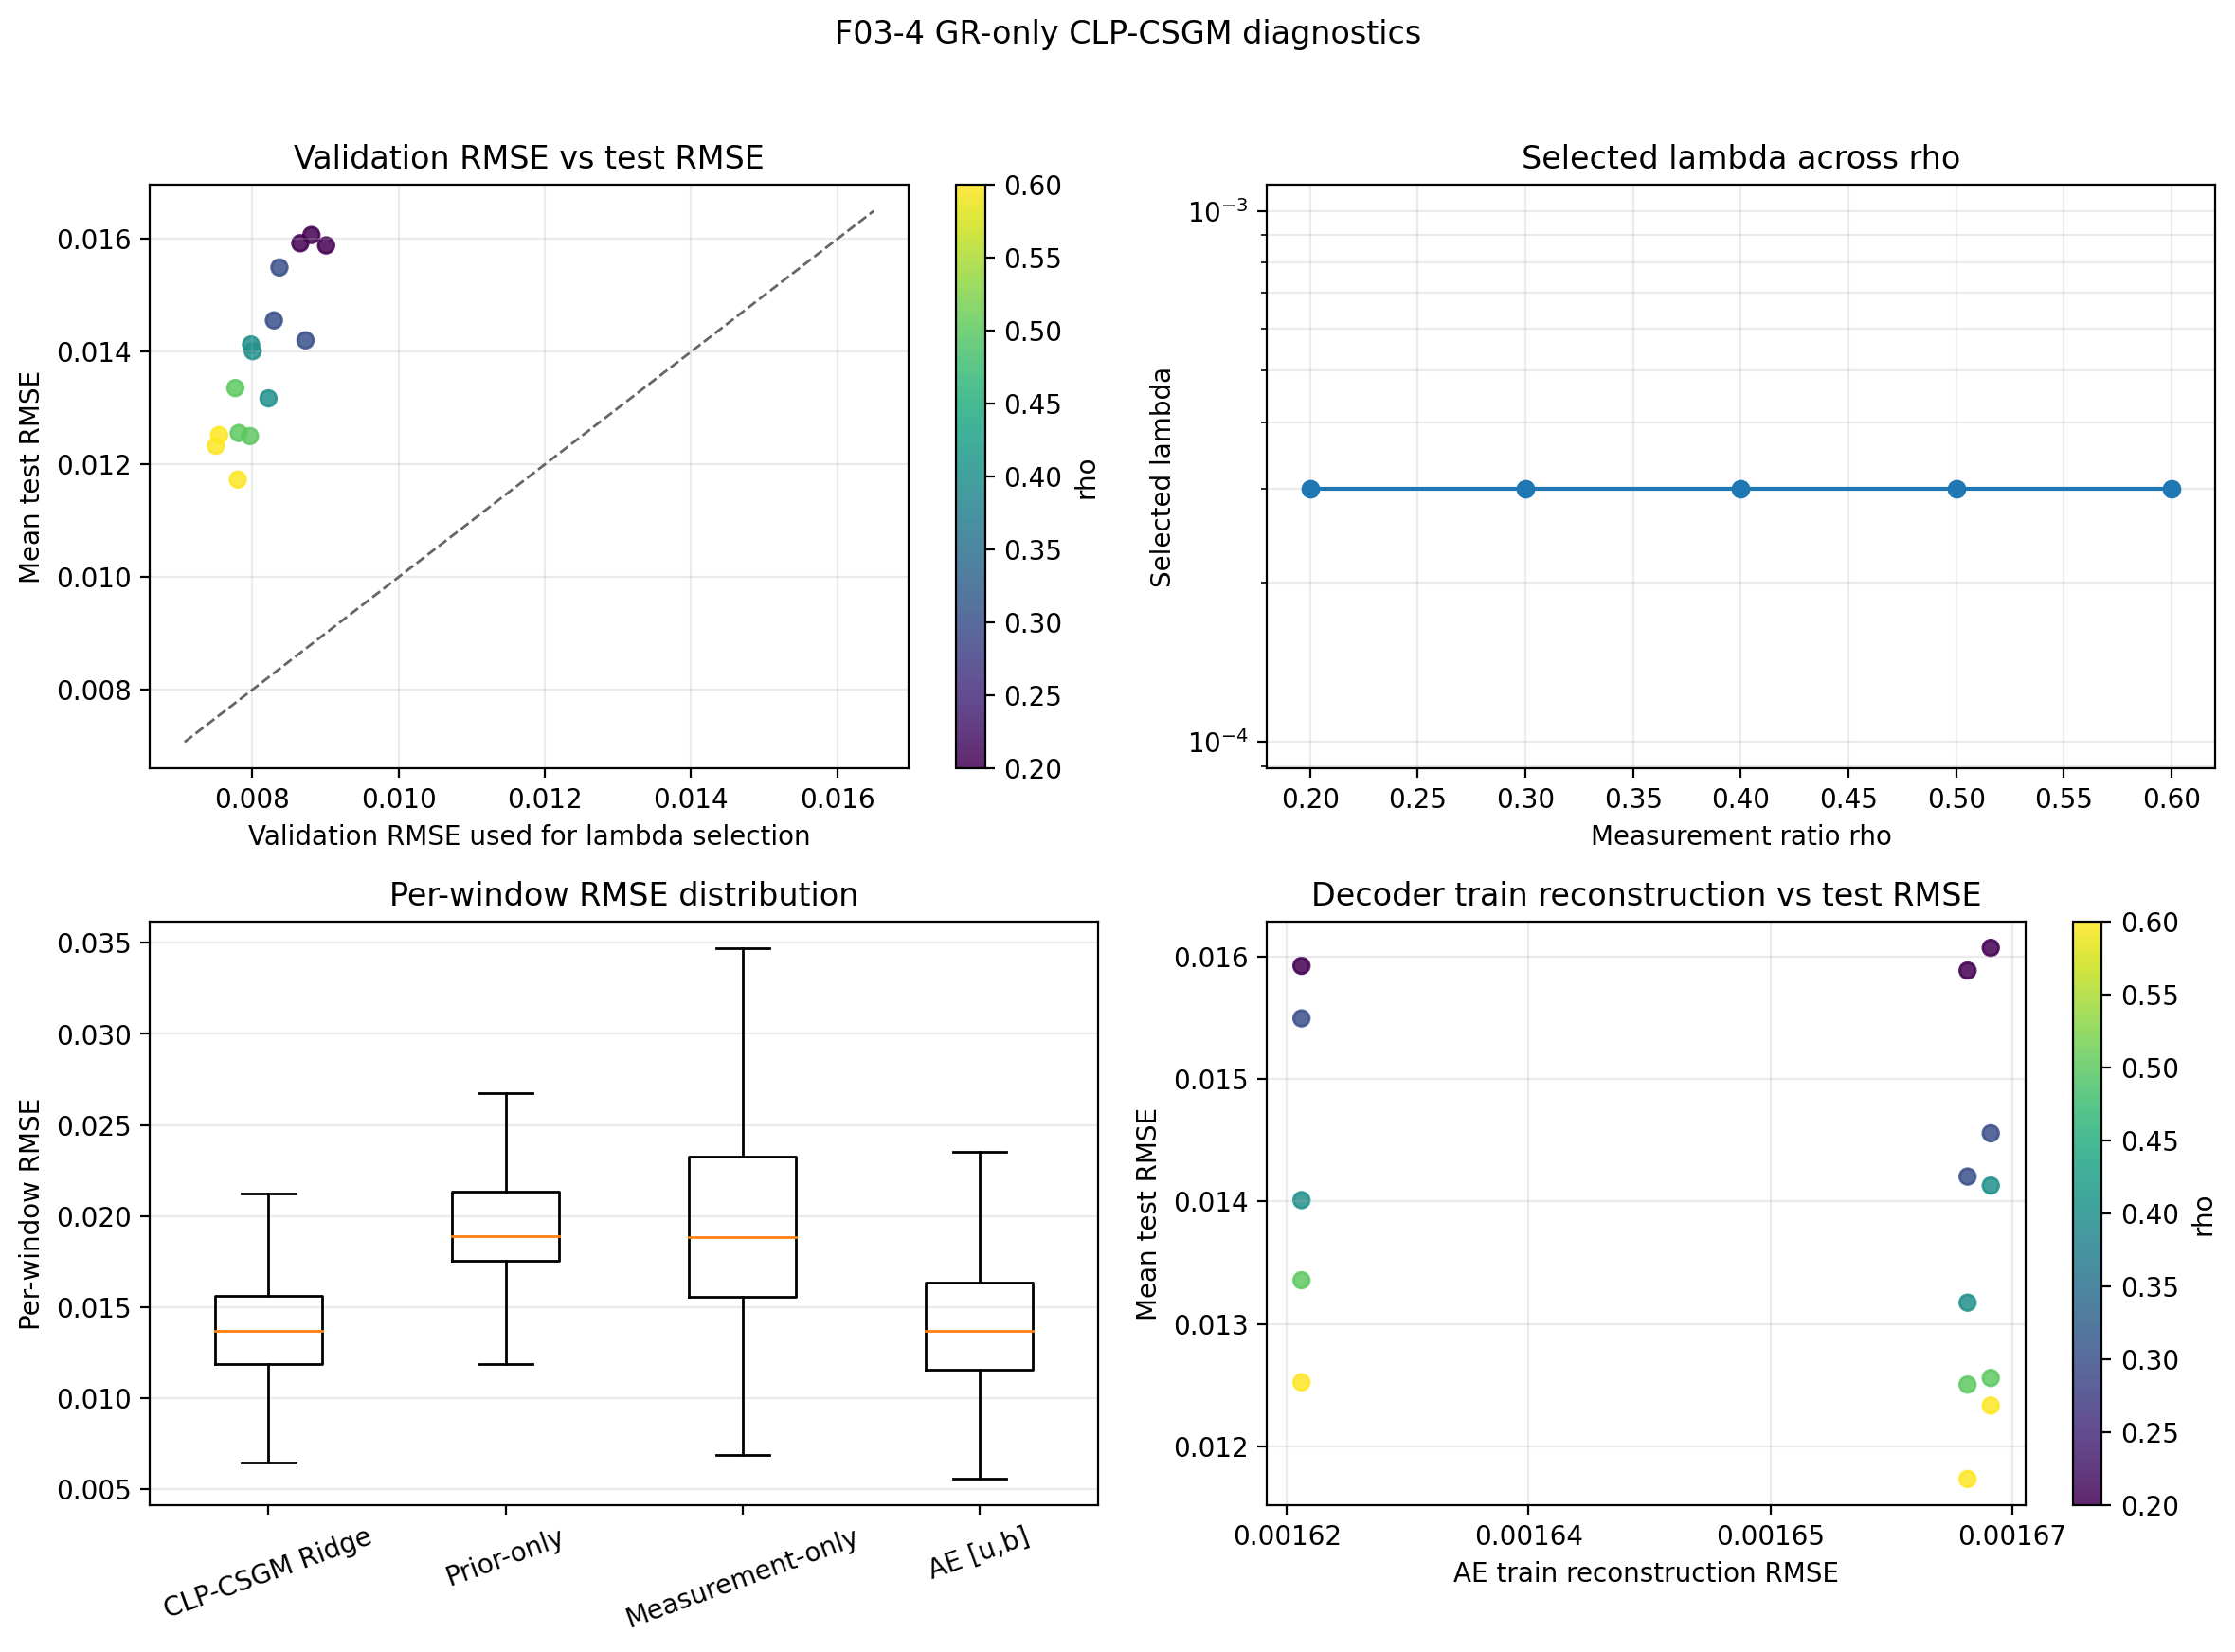
\includegraphics[width=\linewidth]{figures/diagnostic_f03_generalization.png}
  \caption{F03-4 GR-only diagnostics for CLP-CSGM Ridge summarizing the experiments in Section~\ref{subsec:f03_gr_only_results}. The
  panels report validation RMSE versus mean test RMSE, selected \(\lambda\),
  per-window RMSE distributions, and the relation between autoencoder training
  reconstruction error and final test RMSE.}
  \label{fig:diagnostic_f03}
\end{figure}

\subsection{Cross-well Channel-Ablation and Embargo-Style Boundary Check}
\label{app:crosswell_gr_embargo}

This subsection reports a paired robustness check for the cross-well \(V_c\)
step-16 setting. It tests two possible sensitivities: reintroducing GR into
\(u\), relative to the main no-GR protocol in Section~\ref{sec:experiments}, and
removing overlap-prone windows near the train/validation boundary. The latter is
an embargo-style boundary check: a small band of windows adjacent to the boundary
is removed before validation to create a gap between training and validation
windows. We compare four scenarios under the same seeds and measurement-ratio
grid, \(\rho\in\{0.05,0.10,0.20\}\):
\begin{itemize}
  \item No boundary check + GR in \(u\) (stronger dense context reference).
  \item Embargo-style removal (4 boundary windows) + GR in \(u\).
  \item No boundary check + GR excluded from \(u\) (matches the main cross-well \(u\)).
  \item Embargo-style removal (4 boundary windows) + GR excluded from \(u\).
\end{itemize}

Operationally, the embargo-style removal drops four overlap-prone boundary
windows before the validation tail in each training well. In this setup,
\(n_{\mathrm{train}}\) decreases from 52 to 41, while \(n_{\mathrm{val}}\) and
\(n_{\mathrm{test}}\) stay fixed.

\begin{table}[htbp]
  \centering
  \caption{Cross-well step-16 robustness check across GR ablation and
  embargo-style boundary-check scenarios. Ridge RMSE is reported as mean \(\pm\)
  std over three seeds. Gains are relative RMSE reductions of CLP-CSGM Ridge
  against AE \([u,b]\) and measurement-only CSGM.}
  \label{tab:crosswell_gr_embargo_robustness}
  \small
  \adjustbox{max width=\linewidth}{\begin{tabular}{lllllll}
\toprule
scenario & rho & ridge rmse & ae rmse & meas-only rmse & ridge gain vs ae (\%) & ridge gain vs meas-only (\%) \\
\midrule
Emb4+GR & 0.05 & 0.01487 $\pm$ 0.00035 & 0.02056 & 0.03647 & 27.7 & 59.2 \\
Emb4+GR & 0.10 & 0.01406 $\pm$ 0.00032 & 0.01953 & 0.02849 & 28.0 & 50.7 \\
Emb4+GR & 0.20 & 0.01282 $\pm$ 0.00026 & 0.01932 & 0.02167 & 33.6 & 40.8 \\
Emb4-noGR & 0.05 & 0.03117 $\pm$ 0.00020 & 0.03781 & 0.03647 & 17.6 & 14.5 \\
Emb4-noGR & 0.10 & 0.02549 $\pm$ 0.00268 & 0.03439 & 0.02849 & 25.9 & 10.6 \\
Emb4-noGR & 0.20 & 0.01625 $\pm$ 0.00139 & 0.03771 & 0.02167 & 56.9 & 25.0 \\
NoEmb+GR & 0.05 & 0.01403 $\pm$ 0.00064 & 0.01893 & 0.03622 & 25.9 & 61.3 \\
NoEmb+GR & 0.10 & 0.01380 $\pm$ 0.00107 & 0.01802 & 0.02954 & 23.4 & 53.3 \\
NoEmb+GR & 0.20 & 0.01289 $\pm$ 0.00052 & 0.01822 & 0.02127 & 29.3 & 39.4 \\
NoEmb-noGR & 0.05 & 0.03344 $\pm$ 0.00151 & 0.03712 & 0.03622 & 9.9 & 7.7 \\
NoEmb-noGR & 0.10 & 0.02689 $\pm$ 0.00235 & 0.03420 & 0.02954 & 21.4 & 9.0 \\
NoEmb-noGR & 0.20 & 0.01771 $\pm$ 0.00138 & 0.03214 & 0.02127 & 44.9 & 16.7 \\
\bottomrule
\end{tabular}
}
\end{table}

Table~\ref{tab:crosswell_gr_embargo_robustness} shows three stable patterns.
Within each boundary protocol, including GR in \(u\) lowers absolute RMSE, as
expected because \(V_c\) is Larionov-derived from GR. Under the no-GR protocol
matching the main benchmark, CLP-CSGM Ridge has the lowest RMSE relative to AE
\([u,b]\) and measurement-only CSGM throughout the tested grid. The embargo-style
boundary check changes the absolute values without reversing this ordering.
These checks support the main interpretation: the cross-well \(V_c\) benchmark
tests sparse target-log reconstruction under distribution shift without a GR
shortcut in \(u\), and the reported gains are not solely an artifact of
train/validation boundary overlap.

\begin{figure}[htbp]
  \centering
  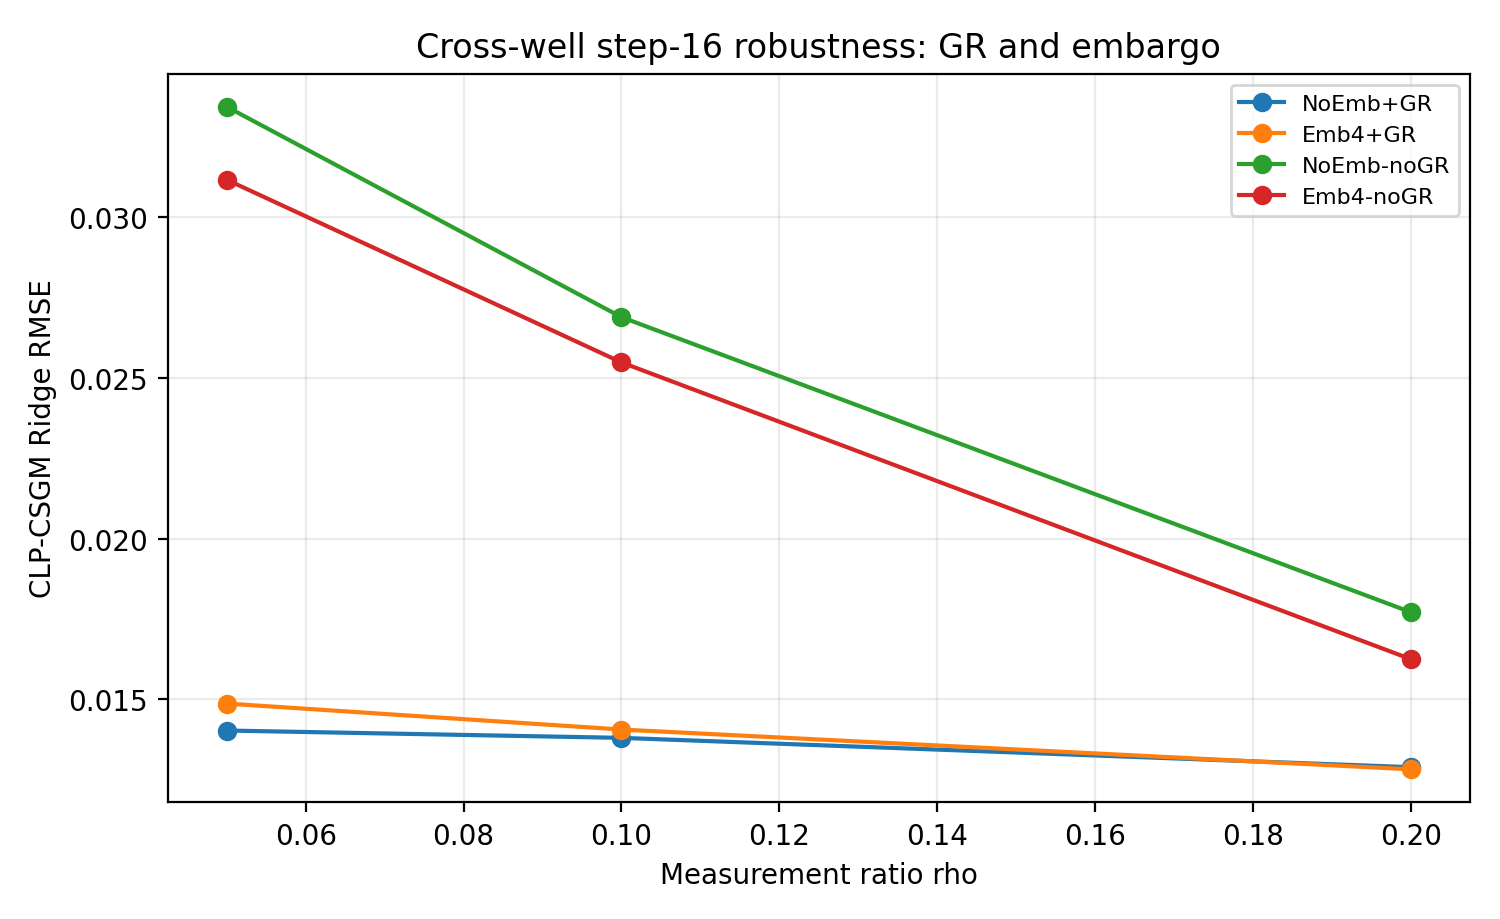
\includegraphics[width=0.92\linewidth]{figures/robustness_crosswell_step16_gr_embargo.png}
  \caption{Cross-well step-16 RMSE sensitivity for CLP-CSGM Ridge across GR
  inclusion in \(u\) and embargo-style boundary-check scenarios. Omitting GR from
  \(u\) relative to GR-inclusive rows increases error; the boundary check shifts
  absolute values without overturning the ranking trends.}
  \label{fig:crosswell_gr_embargo_robustness}
\end{figure}

\subsection{Step-32 development-split resampling}
\label{app:crosswell_step32_dev_splits}

The main cross-well grid uses a depth-tail validation split. At step $32$ the
development pool is small ($n_{\mathrm{train}}=27$, $n_{\mathrm{val}}=3$ after
the split). To test whether the CLP-CSGM Ridge versus AE $[u,b]$ gap in that
cell depends on the particular validation windows, we redrew the same
validation budget ten times inside each development well
(\texttt{random\_per\_well}), keeping F03-4 as the held-out test well and
freezing the sparse coordinates $\Omega$ to the paper seed $7$. Prior-only and
measurement-only ablations were not rerun.

\begin{table}[htbp]
  \centering
  \caption{Cross-well step-$32$ resampling of the development train/validation
  split ($n=10$). RMSE is the mean $\pm$ standard deviation across splits.
  Positive mean $\Delta\mathrm{RMSE}$ (AE $-$ CLP) favors CLP-CSGM Ridge.
  CLP win frac is the fraction of splits with lower CLP RMSE.}
  \label{tab:crosswell_step32_dev_splits}
  \small
  \adjustbox{max width=\linewidth}{\begin{tabular}{rrrrrrrr}
\toprule
$\rho$ & $n_{\mathrm{splits}}$ & $n_{\mathrm{train}}$ & $n_{\mathrm{val}}$ & CLP RMSE & AE RMSE & mean $\Delta$RMSE & CLP win frac \\
\midrule
0.05 & 10 & 27 & 3 & 0.0342 $\pm$ 0.0024 & 0.0407 $\pm$ 0.0025 & 0.0064 & 1.00 \\
0.10 & 10 & 27 & 3 & 0.0305 $\pm$ 0.0032 & 0.0388 $\pm$ 0.0015 & 0.0083 & 1.00 \\
0.20 & 10 & 27 & 3 & 0.0188 $\pm$ 0.0010 & 0.0362 $\pm$ 0.0064 & 0.0174 & 1.00 \\
\bottomrule
\end{tabular}
}
\end{table}

Table~\ref{tab:crosswell_step32_dev_splits} shows that CLP-CSGM Ridge has lower
mean RMSE than AE $[u,b]$ at every tested $\rho$, and lower RMSE in all ten
splits. This check does not add a second held-out well and does not vary
$\Omega$; it only resamples the small development split. Adjacent windows have
length $64$ and step $32$, so they share $32$ depth samples. This
random-per-well redraw does not apply a boundary embargo. In each of the ten
splits, all three validation windows share at least one depth sample with a
training window of the same well ($30$ of $30$ validation windows). One
validation window comes from F02-1 and two from F03-2; F06-1 has only two
windows and stays in the training set. The ten splits test sensitivity to that
development partition. They do not represent independent validation without
shared samples, and they are not ten independent wells.

\subsection{Ten-seed CLP versus AE panel}
\label{app:crosswell_seed_panel}

The main cross-well intervals use three seeds ($t$ critical value with
$\mathrm{df}=2$). Several of those paired $\Delta\mathrm{RMSE}$ intervals
include zero, and the CLP-CSGM Ridge versus AE $[u,b]$ ranking changes between
step $8$ and steps $16$--$32$. We therefore reran that pairwise comparison with
ten seeds $\{7,23,41,13,29,31,37,43,47,53\}$, keeping the submitted tail
validation split, the no-GR input, and F03-4 as the held-out well. Direct MLP
and PCA, structural ablations, and the F03-4 grid were not rerun.

\begin{table}[htbp]
  \centering
  \caption{Cross-well paired
  $\Delta\mathrm{RMSE}=\mathrm{RMSE}_{\mathrm{AE}}-\mathrm{RMSE}_{\mathrm{CLP}}$
  on ten seeds. SE is the seed-level standard error; the $95\%$ half-width uses
  Student-$t$ with $\mathrm{df}=9$. Positive mean $\Delta\mathrm{RMSE}$ favors
  CLP-CSGM Ridge. Wins count seeds with strictly lower RMSE.}
  \label{tab:crosswell_seed_panel}
  \small
  \adjustbox{max width=\linewidth}{\begin{tabular}{rrrrrrrrr}
\toprule
step & $\rho$ & $n$ & mean $\Delta$RMSE & SE & $t$ 95\% half-width & CLP wins & AE wins & CI includes 0 \\
\midrule
8 & 0.05 & 10 & -0.00826 & 0.00121 & 0.00273 & 0 & 10 & no \\
8 & 0.10 & 10 & -0.00318 & 0.00092 & 0.00209 & 2 & 8 & no \\
8 & 0.20 & 10 & 0.00360 & 0.00129 & 0.00293 & 7 & 3 & no \\
16 & 0.05 & 10 & 0.00434 & 0.00159 & 0.00360 & 9 & 1 & no \\
16 & 0.10 & 10 & 0.00677 & 0.00134 & 0.00304 & 10 & 0 & no \\
16 & 0.20 & 10 & 0.01382 & 0.00145 & 0.00328 & 10 & 0 & no \\
32 & 0.05 & 10 & 0.00865 & 0.00129 & 0.00292 & 10 & 0 & no \\
32 & 0.10 & 10 & 0.01217 & 0.00118 & 0.00266 & 10 & 0 & no \\
32 & 0.20 & 10 & 0.01934 & 0.00185 & 0.00418 & 10 & 0 & no \\
\bottomrule
\end{tabular}
}
\end{table}

Table~\ref{tab:crosswell_seed_panel} shows that none of the nine ten-seed
intervals include zero. The CLP-CSGM Ridge advantage is concentrated where
training support is smallest (steps $16$ and $32$, $52$ and $27$ training
windows): lower RMSE at every $\rho$. At step $8$, where the training set is
largest ($104$ training windows), AE $[u,b]$ has lower RMSE at
$\rho=0.05$ and $\rho=0.10$; CLP-CSGM Ridge has lower RMSE only at
$\rho=0.20$. This is a low-training-support pattern, not a uniform gain at
every small measurement ratio. The submitted three-seed tables are unchanged.
Each interval describes variability across the ten seeds on the single
held-out well F03-4. It is not evidence of generalization across wells, and
the ten seeds are not ten independent geological tests. The
nine intervals are separate cell summaries, not a simultaneous
multiplicity-corrected test, and overlapping windows are not counted as extra
independent samples. Each of these seeds also draws its own coordinates and
measurement noise, so the panel does not separate training randomness from
the observation realization.
Appendix~\ref{app:crosswell_omega_placement} holds the model seeds fixed and
redraws those coordinates together with the measurement noise, without
isolating placement from noise.

\subsection{Explicit-mask direct AE}
\label{app:crosswell_explicit_mask}

The main direct baselines receive $[\boldsymbol{u},\boldsymbol{b}]$ with
positional identity implicit in the column order. CLP-CSGM instead applies
$M_{\Omega}$ to the length-$N$ window. To test whether the CLP-CSGM gain is
only that coordinate placement, we fit one additional direct AE on the same
nine cells, seeds, and noise. Its input is
$[\boldsymbol{u},\boldsymbol{b}_{\Omega},\mathrm{mask}]$:
$\boldsymbol{b}_{\Omega}\in\mathbb{R}^{N}$ holds the noisy measurement at each
observed coordinate and zero elsewhere, and the mask is the binary indicator
of $\Omega$. Numeric channels are standardized from the training windows only.
The trailing binary mask is left unscaled, so its entries remain in
$\{0,1\}$. The mask-aware AE uses the same base training seed as the
conventional AE. Both direct models and CLP-CSGM Ridge share the same
partitions, observation coordinates, and noisy target measurements within
each cell. MLP, PCA, ablations, and the F03-4 grid were not rerun, and this
method is not added to the main tables.

An earlier historical run scaled the full concatenated vector and trained
the masked AE at seed offset $100$. That preprocessing zeroed the constant
mask columns. The difference between that historical variant and the
corrected protocol cannot be attributed to either change alone.

\begin{table}[htbp]
  \centering
  \caption{Cross-well CLP-CSGM Ridge versus AE $[\boldsymbol{u},\boldsymbol{b}]$
  and an AE that also receives an explicit window mask ($n=3$ seeds).
  $\Delta$ is the other method's RMSE minus CLP RMSE. Positive $\Delta$ favors
  CLP-CSGM Ridge. Wins count seeds with strictly lower CLP RMSE.}
  \label{tab:crosswell_explicit_mask}
  \small
  \adjustbox{max width=\linewidth}{\begin{tabular}{rrrrrrrrr}
\toprule
step & $\rho$ & CLP & AE $[u,b]$ & AE mask & $\Delta$ AE & $\Delta$ mask & CLP$>$AE & CLP$>$mask \\
\midrule
8 & 0.05 & 0.0448 & 0.0357 & 0.0346 & -0.0092 & -0.0102 & 0/3 & 0/3 \\
8 & 0.10 & 0.0365 & 0.0320 & 0.0312 & -0.0045 & -0.0053 & 1/3 & 0/3 \\
8 & 0.20 & 0.0227 & 0.0260 & 0.0260 & 0.0033 & 0.0034 & 2/3 & 3/3 \\
16 & 0.05 & 0.0334 & 0.0371 & 0.0346 & 0.0037 & 0.0011 & 3/3 & 2/3 \\
16 & 0.10 & 0.0269 & 0.0342 & 0.0322 & 0.0073 & 0.0053 & 3/3 & 3/3 \\
16 & 0.20 & 0.0177 & 0.0321 & 0.0281 & 0.0144 & 0.0103 & 3/3 & 3/3 \\
32 & 0.05 & 0.0322 & 0.0390 & 0.0389 & 0.0068 & 0.0067 & 3/3 & 3/3 \\
32 & 0.10 & 0.0264 & 0.0389 & 0.0376 & 0.0125 & 0.0112 & 3/3 & 3/3 \\
32 & 0.20 & 0.0170 & 0.0396 & 0.0348 & 0.0225 & 0.0178 & 3/3 & 3/3 \\
\bottomrule
\end{tabular}
}
\end{table}

The corrected explicit-mask AE preserves the binary mask without centering or
standardization and uses the same base training seed as the conventional AE.
Both direct models and CLP-CSGM Ridge are evaluated using the same data
partitions, observation coordinates, and noisy target measurements within
each cell.

CLP-CSGM Ridge achieves lower mean RMSE than the mask-aware AE in seven of
the nine cross-well configurations. At steps $16$ and $32$, corresponding to
the smaller training sets, CLP-CSGM Ridge has lower mean RMSE in all six
configurations and lower RMSE in $17$ of the $18$ paired seed comparisons.
At step $8$, the mask-aware AE remains better at measurement ratios $0.05$
and $0.10$.

Because the sampling coordinates are fixed within each configuration, the
binary mask is constant across windows, and the conventional AE already
receives the measurements in a consistent positional order. The experiment
therefore assesses an alternative explicit spatial encoding, but does not
isolate the causal effect of latent inverse optimization. The placement
check is Appendix~\ref{app:crosswell_omega_placement}.

\subsection{Sparse-coordinate placement}
\label{app:crosswell_omega_placement}

The main protocol samples one coordinate set $\Omega$ for each model seed and
measurement ratio and then holds it fixed across windows. To check stability
under new sparse-observation realizations, we redrew $\Omega$ and the
measurement noise five times on the cross-well $V_c$ grid.
The model seeds stay at $\{7,23,41\}$, so the decoder and the ridge anchor
keep the same initialization. The first draw is the published coordinate set
and noise realization.
The other four draws change only the generator that samples $\Omega$ and the
noise on $\boldsymbol{b}$, so the positions and the noise change together.
This check does not isolate the effect of position from the effect of noise.
The direct AE is fit again on each draw, because
$\boldsymbol{b}$ is part of its input, and the CLP-CSGM penalty weight is
selected again on the validation windows of that draw. The score is the same
full-window RMSE as the main grid. Direct MLP, PCA, structural ablations, and
the F03-4 grid were not rerun, and these draws are not merged into the
submitted three-seed tables.

\begin{table}[htbp]
  \centering
  \caption{Cross-well CLP-CSGM Ridge versus AE $[\boldsymbol{u},\boldsymbol{b}]$
  across five sparse-coordinate placements and the three paper seeds
  ($n=15$ per cell). RMSE values are means over those comparisons.
  Positive mean $\Delta\mathrm{RMSE}$ (AE $-$ CLP) favors CLP-CSGM Ridge.
  Wins count comparisons with strictly lower RMSE.}
  \label{tab:crosswell_omega_placement}
  \small
  \adjustbox{max width=\linewidth}{\begin{tabular}{rrrrrrrr}
\toprule
step & $\rho$ & $n$ & CLP RMSE & AE RMSE & mean $\Delta$RMSE & CLP wins & AE wins \\
\midrule
8 & 0.05 & 15 & 0.04231 & 0.03586 & -0.00645 & 0 & 15 \\
8 & 0.10 & 15 & 0.03581 & 0.03225 & -0.00356 & 5 & 10 \\
8 & 0.20 & 15 & 0.02383 & 0.02591 & 0.00208 & 11 & 4 \\
16 & 0.05 & 15 & 0.03072 & 0.03710 & 0.00638 & 15 & 0 \\
16 & 0.10 & 15 & 0.02615 & 0.03412 & 0.00797 & 15 & 0 \\
16 & 0.20 & 15 & 0.01840 & 0.03036 & 0.01196 & 15 & 0 \\
32 & 0.05 & 15 & 0.02895 & 0.03873 & 0.00977 & 15 & 0 \\
32 & 0.10 & 15 & 0.02470 & 0.03870 & 0.01401 & 15 & 0 \\
32 & 0.20 & 15 & 0.01795 & 0.04023 & 0.02228 & 15 & 0 \\
\bottomrule
\end{tabular}
}
\end{table}

Table~\ref{tab:crosswell_omega_placement} shows that the cell-level winner
matches the published ranking in all nine cells. At steps $16$ and $32$,
CLP-CSGM Ridge has lower RMSE in all fifteen comparisons at every $\rho$.
At step $8$ and $\rho=0.05$, AE $[\boldsymbol{u},\boldsymbol{b}]$ is lower in
all fifteen. The two closer step-$8$ cells are not unanimous: five of fifteen
comparisons favor CLP-CSGM Ridge at $\rho=0.10$, and four of fifteen favor
the direct AE at $\rho=0.20$. The low-training-support advantage therefore
does not depend on the one published observation draw. The step-$8$ ranking is
the less stable of the two regimes, and a single extra draw can reverse an
individual seed there. These fifteen comparisons are three model seeds times
five draws on the single held-out well F03-4. They are not fifteen independent
wells, and they are not evidence of cross-well generalization. This check does
not add seeds beyond $\{7,23,41\}$.

\subsection{Direct linear maps, depth interpolation, and measurement noise}
\label{app:crosswell_simple_baselines}

The main grid does not include a direct linear map from
$[\boldsymbol{u},\boldsymbol{b}]$ or an interpolation of the sparse
measurements. This supplement adds both on the cross-well $V_c$ grid, with
the same windows, seeds $\{7,23,41\}$, measurement ratios, and published
coordinate draws. Ordinary least squares and ridge regression map
standardized $[\boldsymbol{u},\boldsymbol{b}]$ to the window. The ridge
penalty is chosen on validation full-window RMSE. Interpolation connects the
noisy measurements along the depth index of the window and keeps the nearest
measured value at the ends. It does not use the dense logs. The score is the
same full-window RMSE as the main grid. CLP-CSGM Ridge and AE
$[\boldsymbol{u},\boldsymbol{b}]$ in
Table~\ref{tab:crosswell_simple_baselines} are the published offset-$0$ runs.
These comparators are not merged into the submitted tables.

\begin{table}[htbp]
  \centering
  \caption{Cross-well full-window RMSE at the published noise standard
  deviation $0.01$. Values are means over seeds $\{7,23,41\}$.
  Linear $[u,b]$ is ordinary least squares and Ridge direct is
  validation-selected ridge, both from $[\boldsymbol{u},\boldsymbol{b}]$ to
  the window. Interpolation uses only the sparse measurements.
  The lowest value in every cell is interpolation.}
  \label{tab:crosswell_simple_baselines}
  \small
  \adjustbox{max width=\linewidth}{\begin{tabular}{rrrrrrr}
\toprule
step & $\rho$ & Linear $[u,b]$ & Ridge direct & Interpolation & CLP-CSGM & AE $[u,b]$ \\
\midrule
8 & 0.05 & 0.03122 & 0.02916 & 0.01779 & 0.04483 & 0.03567 \\
8 & 0.10 & 0.02790 & 0.02384 & 0.01537 & 0.03646 & 0.03195 \\
8 & 0.20 & 0.02158 & 0.01862 & 0.01100 & 0.02267 & 0.02600 \\
16 & 0.05 & 0.02903 & 0.02910 & 0.01751 & 0.03344 & 0.03712 \\
16 & 0.10 & 0.02634 & 0.02661 & 0.01478 & 0.02689 & 0.03420 \\
16 & 0.20 & 0.02062 & 0.02089 & 0.01115 & 0.01771 & 0.03214 \\
32 & 0.05 & 0.03382 & 0.03980 & 0.01755 & 0.03217 & 0.03901 \\
32 & 0.10 & 0.03083 & 0.03878 & 0.01533 & 0.02640 & 0.03894 \\
32 & 0.20 & 0.02421 & 0.02648 & 0.01125 & 0.01705 & 0.03959 \\
\bottomrule
\end{tabular}
}
\end{table}

Table~\ref{tab:crosswell_simple_baselines} shows that interpolation has the
lowest RMSE in all nine cells. Seed by seed, it is also lowest in all $27$
comparisons. CLP-CSGM Ridge is lower than both direct linear maps at step
$16$, $\rho=0.20$, and at step $32$ for every $\rho$. At step $8$, and at
step $16$ for $\rho=0.05$ and $\rho=0.10$, one or both linear maps are lower
than CLP-CSGM Ridge. The measurements at this noise level are a slightly
perturbed copy of the same smooth curve, so connecting them is enough.

The same windows and the same standard-normal draws are scaled to noise
standard deviations $0.01$, $0.05$, $0.10$, and $0.20$.
Table~\ref{tab:crosswell_noise_sweep} and
Fig.~\ref{fig:crosswell_rmse_vs_noise} use one refit of that series.
The decoder and the dense-log map are fit once per step and seed, without
the sparse measurements. For each measurement fraction and each noise
level, the penalty weight is selected again on validation full-window RMSE.
The reported CLP-CSGM values are that selected-penalty result, not a
reconstruction with one fixed weight. The sensitivity sweep uses a
different, wider grid, with candidates $10^{-4}$, $10^{-3}$, $10^{-2}$,
$10^{-1}$, $1$, $10$, and $100$. It omits the factor-of-three candidates
from the published grid. At $0.01$ and at $0.05$ every selected weight also
belongs to the published grid. That membership does not mean the two
searches were the same. At noise $0.10$, step $16$ and
$\rho=0.10$, one seed selects the weight $1$, above the published grid and still
inside the sweep. At noise $0.20$, some cells select
$100$, the largest candidate that was tried. That selection is not an
optimum outside the searched grid. At noise $0.01$ the ordering matches
Table~\ref{tab:crosswell_simple_baselines}, but the cell means are those of
this refit. At step $16$ and $\rho=0.20$, the published CLP-CSGM mean is
$0.01771$ and the refit mean is $0.0159$. In that cell the selected weight
is $0.0001$, inside the published grid. The held-out curve has standard
deviation $0.035$. The window predicted from the dense logs alone, with no
measurement term, has mean RMSE $0.0564$ at step $8$, $0.0426$ at step
$16$, and $0.0432$ at step $32$.

\begin{table}[htbp]
  \centering
  \caption{Interpolation versus CLP-CSGM Ridge when only the measurement-noise
  standard deviation changes. RMSE values are means over the three paper
  seeds. Wins count seeds in which CLP-CSGM Ridge has strictly lower RMSE.
  The held-out $V_c$ standard deviation is $0.035$, on the same scale as the
  noise. Noise $0.05$ is about $1.43$ times that deviation. Noise levels
  $0.10$ and $0.20$ are about $2.86$ and $5.71$ times that deviation.
  These noise levels were used for sensitivity analysis and were not
  calibrated to field measurement uncertainties. The decoder and the
  dense-log map are fit once per
  step and seed, and the penalty is selected on validation at each noise
  level. Noise $0.01$ in this table is that refit. At $0.20$ some selected
  weights equal $100$, the largest candidate on this grid, which is not an
  optimum outside the grid.}
  \label{tab:crosswell_noise_sweep}
  \small
  \adjustbox{max width=\linewidth}{\begin{tabular}{rrrrrrrrrrrrrr}
\toprule
& & \multicolumn{3}{c}{$\sigma_{\eta}=0.01$} & \multicolumn{3}{c}{$\sigma_{\eta}=0.05$} & \multicolumn{3}{c}{$\sigma_{\eta}=0.10$} & \multicolumn{3}{c}{$\sigma_{\eta}=0.20$} \\
\cmidrule(lr){3-5} \cmidrule(lr){6-8} \cmidrule(lr){9-11} \cmidrule(lr){12-14}
step & $\rho$ & Interp. & CLP & wins & Interp. & CLP & wins & Interp. & CLP & wins & Interp. & CLP & wins \\
\midrule
8 & 0.05 & 0.0178 & 0.0456 & 0 & 0.0456 & 0.0508 & 1 & 0.0864 & 0.0547 & 3 & 0.1703 & 0.0557 & 3 \\
8 & 0.10 & 0.0154 & 0.0365 & 0 & 0.0442 & 0.0456 & 1 & 0.0853 & 0.0539 & 3 & 0.1690 & 0.0555 & 3 \\
8 & 0.20 & 0.0110 & 0.0212 & 0 & 0.0423 & 0.0372 & 3 & 0.0838 & 0.0513 & 3 & 0.1673 & 0.0548 & 3 \\
16 & 0.05 & 0.0175 & 0.0334 & 0 & 0.0442 & 0.0386 & 3 & 0.0838 & 0.0416 & 3 & 0.1653 & 0.0424 & 3 \\
16 & 0.10 & 0.0148 & 0.0269 & 0 & 0.0427 & 0.0352 & 3 & 0.0825 & 0.0416 & 3 & 0.1636 & 0.0424 & 3 \\
16 & 0.20 & 0.0112 & 0.0159 & 0 & 0.0428 & 0.0286 & 3 & 0.0847 & 0.0387 & 3 & 0.1690 & 0.0424 & 3 \\
32 & 0.05 & 0.0175 & 0.0317 & 0 & 0.0430 & 0.0382 & 3 & 0.0820 & 0.0423 & 3 & 0.1625 & 0.0430 & 3 \\
32 & 0.10 & 0.0153 & 0.0264 & 0 & 0.0445 & 0.0365 & 3 & 0.0860 & 0.0414 & 3 & 0.1706 & 0.0431 & 3 \\
32 & 0.20 & 0.0112 & 0.0170 & 0 & 0.0425 & 0.0279 & 3 & 0.0840 & 0.0381 & 3 & 0.1674 & 0.0409 & 3 \\
\bottomrule
\end{tabular}
}
\end{table}

At noise standard deviation $0.05$, CLP-CSGM Ridge is lower in every seed at
steps $16$ and $32$ and at step $8$ for $\rho=0.20$. At step $8$ for
$\rho=0.05$ and $\rho=0.10$, interpolation still has the lower mean.
At $0.10$ and $0.20$, CLP-CSGM Ridge is lower in all nine cells and in all
three seeds. Figure~\ref{fig:crosswell_rmse_vs_noise} shows this ordering
with one panel per step. The smaller change in the CLP-CSGM RMSE is not
attributed here to the conditional penalty alone. This supplement does not
separate that penalty from the decoder restriction or from the validation
choice of the weight.
Fig.~\ref{fig:crosswell_noise_panels} shows one held-out interval at the
published noise and at noise $0.05$. The two panels use separate horizontal
scales. Panel (b) is not one of the larger sensitivity levels. In this
displayed interval, interpolation closely follows the reference at noise
standard deviation $0.01$. At $0.05$, it exhibits larger excursions, while
CLP-CSGM Ridge retains more of the broad profile structure. The example is
consistent with the cell-level result for the corresponding configuration,
step $32$ and $\rho=0.20$, and it does not extend to every configuration at
that noise level.

The same observation stream is also scored with a second-difference smoother.
For each window it solves
$\|M_{\Omega}\boldsymbol{y}-\boldsymbol{b}\|_2^2+\alpha\|D^{2}\boldsymbol{y}\|_2^2$,
where $D^{2}$ is the second difference along the window index. The smoother
does not use the dense logs. $\alpha$ is chosen only by validation
full-window RMSE, from the frozen grid
$10^{-6}$, $10^{-4}$, $10^{-2}$, $1$, $10^{2}$, $10^{4}$, and $10^{6}$.
Equal validation scores keep the smaller value. Test targets are not used,
and the grid was not changed after the test scores were known. CLP-CSGM was
not refit. The largest grid value is selected in 62 of the 108 seed rows,
and the smallest value is never selected. A selection at the ceiling is the
best candidate inside the grid, not an optimum beyond it.

\begin{table}[htbp]
  \centering
  \caption{Interpolation, validation-selected second-difference smoothing, and
  CLP-CSGM Ridge on the noise sweep. Entries are mean full-window RMSE over
  seeds $\{7,23,41\}$, rounded to four decimals. The smoother does not use
  the dense logs. These noise levels were used for sensitivity analysis and
  were not calibrated to field measurement uncertainties.}
  \label{tab:crosswell_smooth}
  \small
  \adjustbox{max width=\linewidth}{\begin{tabular}{rrrrrrrrrrrrrr}
\toprule
& & \multicolumn{3}{c}{$\sigma_{\eta}=0.01$} & \multicolumn{3}{c}{$\sigma_{\eta}=0.05$} & \multicolumn{3}{c}{$\sigma_{\eta}=0.10$} & \multicolumn{3}{c}{$\sigma_{\eta}=0.20$} \\
\cmidrule(lr){3-5} \cmidrule(lr){6-8} \cmidrule(lr){9-11} \cmidrule(lr){12-14}
step & $\rho$ & Interp. & Smooth & CLP & Interp. & Smooth & CLP & Interp. & Smooth & CLP & Interp. & Smooth & CLP \\
\midrule
8 & 0.05 & 0.0178 & 0.0251 & 0.0456 & 0.0456 & 0.0646 & 0.0508 & 0.0864 & 0.1232 & 0.0547 & 0.1703 & 0.2437 & 0.0557 \\
8 & 0.10 & 0.0154 & 0.0181 & 0.0365 & 0.0442 & 0.0394 & 0.0456 & 0.0853 & 0.0721 & 0.0539 & 0.1690 & 0.1404 & 0.0555 \\
8 & 0.20 & 0.0110 & 0.0110 & 0.0212 & 0.0423 & 0.0225 & 0.0372 & 0.0838 & 0.0389 & 0.0513 & 0.1673 & 0.0743 & 0.0548 \\
16 & 0.05 & 0.0175 & 0.0246 & 0.0334 & 0.0442 & 0.0589 & 0.0386 & 0.0838 & 0.1302 & 0.0416 & 0.1653 & 0.2548 & 0.0424 \\
16 & 0.10 & 0.0148 & 0.0181 & 0.0269 & 0.0427 & 0.0385 & 0.0352 & 0.0825 & 0.0706 & 0.0416 & 0.1636 & 0.1375 & 0.0424 \\
16 & 0.20 & 0.0112 & 0.0120 & 0.0159 & 0.0428 & 0.0237 & 0.0286 & 0.0847 & 0.0418 & 0.0387 & 0.1690 & 0.0801 & 0.0424 \\
32 & 0.05 & 0.0175 & 0.0429 & 0.0317 & 0.0430 & 0.0759 & 0.0382 & 0.0820 & 0.1177 & 0.0423 & 0.1625 & 0.2326 & 0.0430 \\
32 & 0.10 & 0.0153 & 0.0183 & 0.0264 & 0.0445 & 0.0442 & 0.0365 & 0.0860 & 0.1104 & 0.0414 & 0.1706 & 0.2157 & 0.0431 \\
32 & 0.20 & 0.0112 & 0.0114 & 0.0170 & 0.0425 & 0.0224 & 0.0279 & 0.0840 & 0.0395 & 0.0381 & 0.1674 & 0.0751 & 0.0409 \\
\bottomrule
\end{tabular}
}
\end{table}

Table~\ref{tab:crosswell_smooth} and
Fig.~\ref{fig:crosswell_smooth} keep every cell. At noise $0.01$, smoothing
has lower mean RMSE than CLP-CSGM in eight of nine cells. The exception is
step $32$ and $\rho=0.05$, where the smoother mean is $0.0429$ and the
CLP-CSGM mean is $0.0317$. Interpolation remains lower than CLP-CSGM in all
nine cells at that noise. At $0.05$, CLP-CSGM has the lower mean in five
cells and smoothing in four: step $8$ at $\rho=0.10$ and $\rho=0.20$, and
steps $16$ and $32$ at $\rho=0.20$. At $0.10$, CLP-CSGM is lower in eight
cells, and smoothing is lower at step $8$ and $\rho=0.20$. At $0.20$,
CLP-CSGM is lower in all nine cells. At $\rho=0.05$, the smoother mean is
higher than interpolation at every noise level in the table. The comparison
does not establish general superiority, and it does not isolate the
conditional penalty, the decoder restriction, or the validation choice as a
separate mechanism.

An affine least-squares fit to the same noisy observations is an additional
comparator, not a replacement for the selected smoother. It has no penalty
weight. It is the second-difference problem as $\alpha\to\infty$. On all
108 rows, the curve at $\alpha=10^{6}$ and this affine curve differ by a
median mean-window profile RMSE of $5.2\times10^{-5}$ and a maximum of
$3.7\times10^{-4}$. The largest absolute gap in the scored full-window RMSE
is $2.0\times10^{-5}$. On the 62 ceiling rows the profile median is
$7.6\times10^{-5}$ and the largest scored-RMSE gap is $1.9\times10^{-5}$.
Those ceiling solutions are already near the affine limit
(Fig.~\ref{fig:crosswell_smooth_affine}). The selected smoother can still
differ from that limit when validation chooses an interior weight. At noise
$0.01$ the affine cell mean is lower than CLP-CSGM in all nine cells. In
the step-$32$, $\rho=0.05$ cell, only one of three seeds selects the
ceiling: the affine mean there is $0.0240$, against the selected-smoother
mean $0.0429$ and the CLP-CSGM mean $0.0317$.

\begin{figure}[htbp]
  \centering
  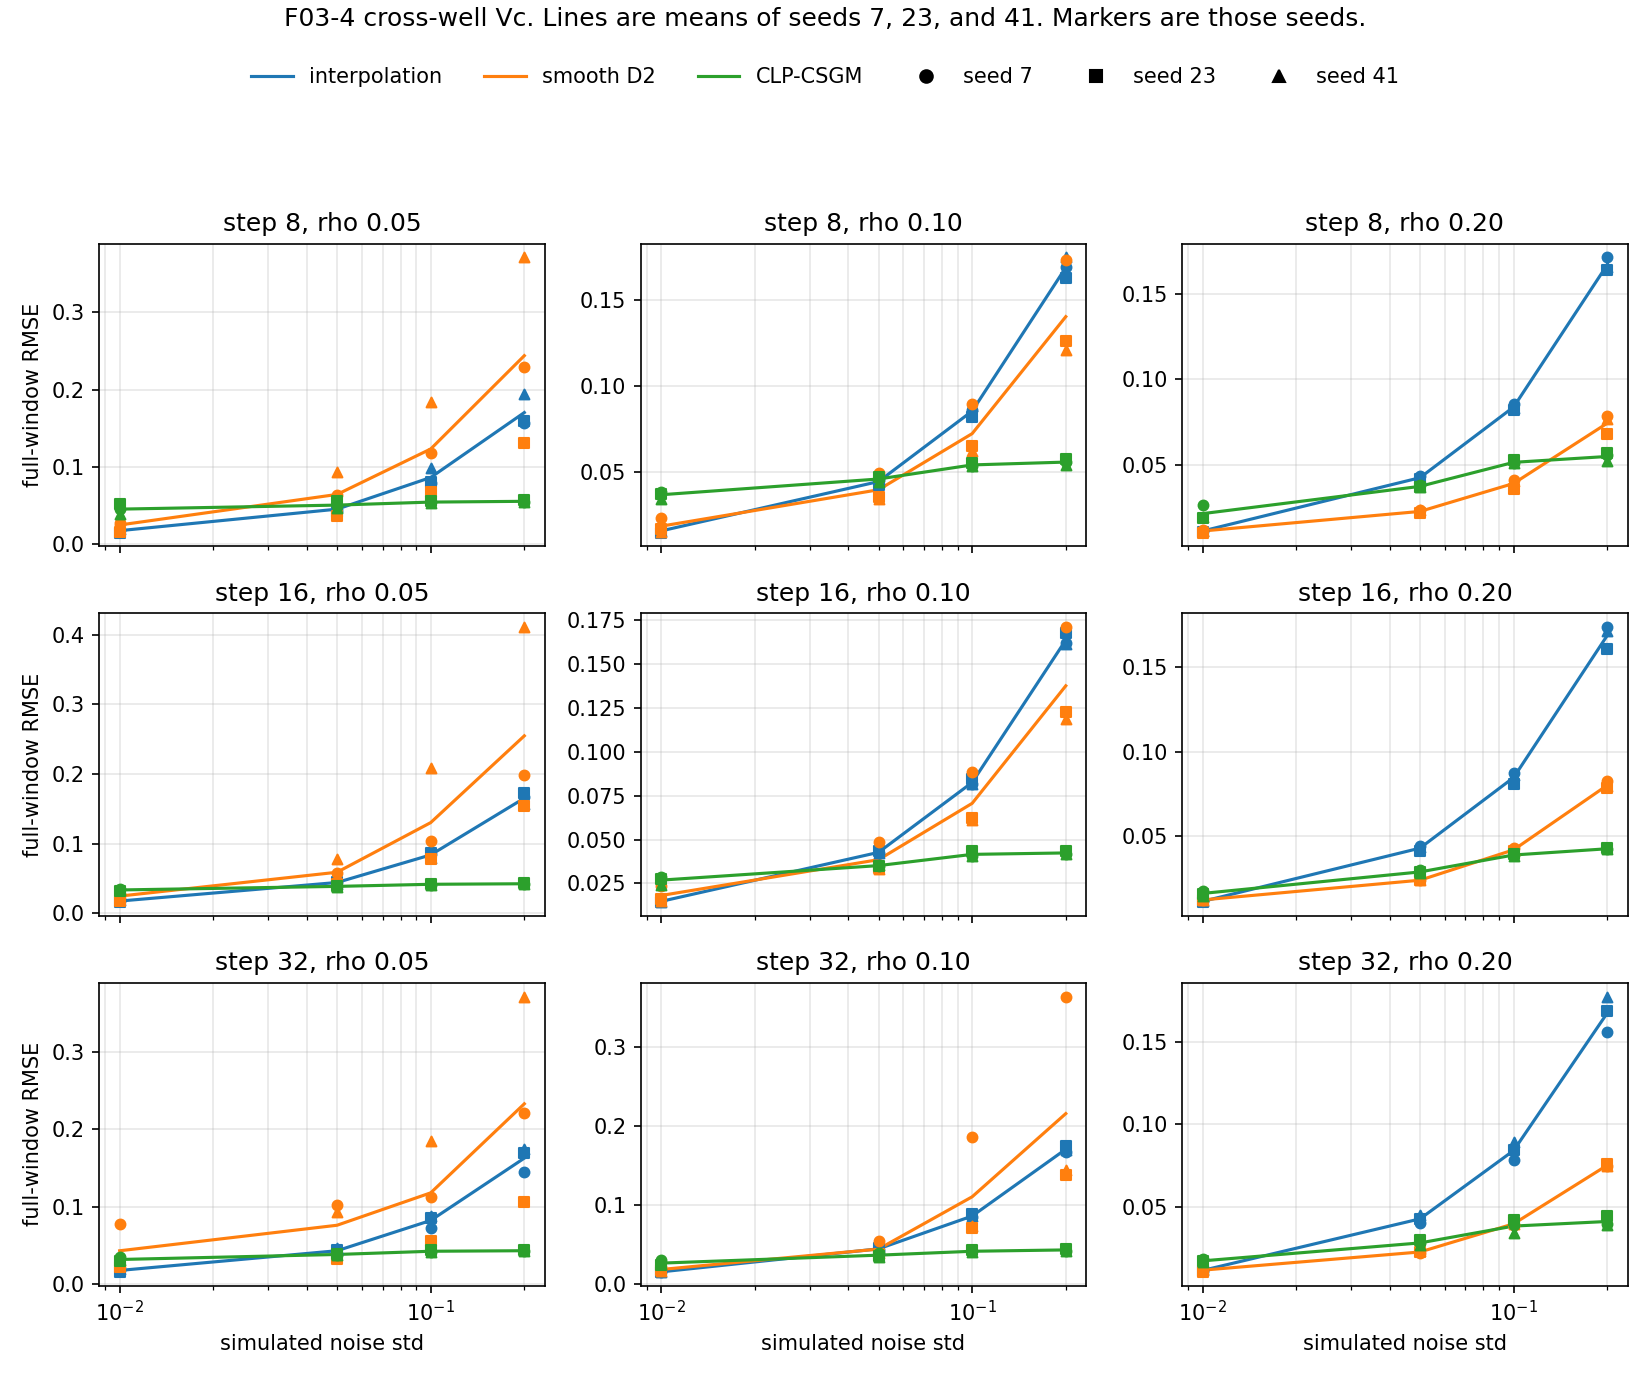
\includegraphics[width=\linewidth]{crosswell_vc_smooth_vs_clp.png}
  \caption{Full-window RMSE of interpolation, validation-selected
  second-difference smoothing, and CLP-CSGM Ridge. Each panel is one step
  and one measurement fraction on held-out F03-4. Lines are means of seeds
  $7$, $23$, and $41$; markers are those seeds. The noise levels are
  simulated and were not calibrated to field measurement uncertainties.}
  \label{fig:crosswell_smooth}
\end{figure}

\begin{figure}[htbp]
  \centering
  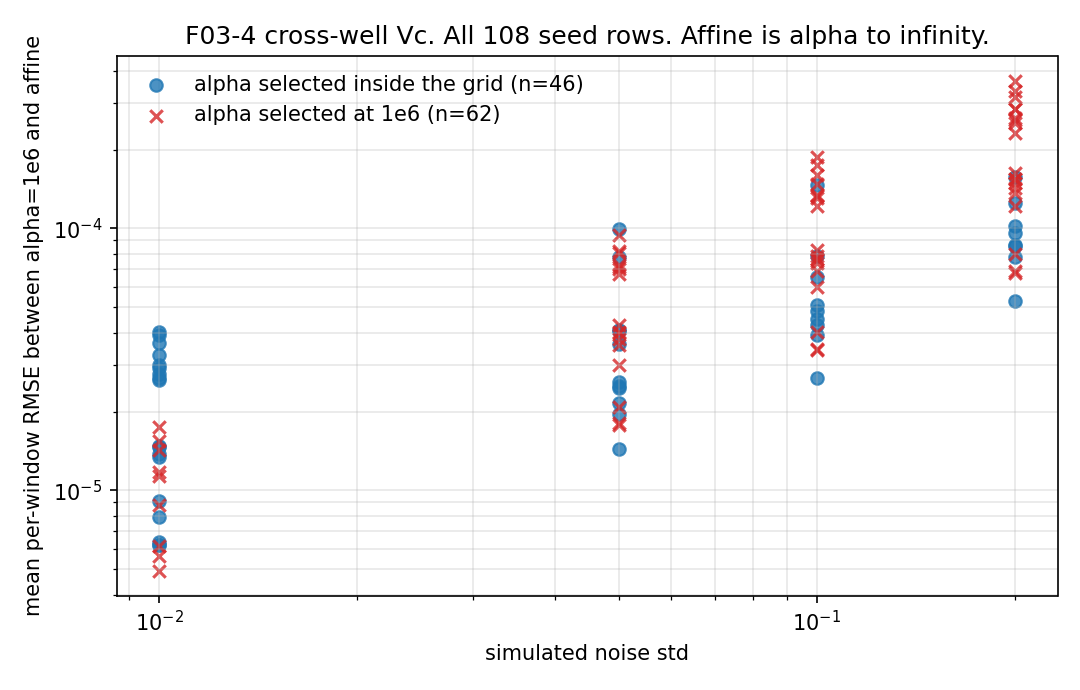
\includegraphics[width=0.92\linewidth]{crosswell_vc_smooth_affine_gap.png}
  \caption{Mean per-window RMSE between the $\alpha=10^{6}$ reconstruction
  and the affine least-squares fit, for all 108 seed rows. Crosses are the
  62 rows whose validation choice is the grid ceiling. Circles are the 46
  rows with an interior choice. The vertical coordinate is the profile gap
  at fixed $\alpha=10^{6}$, not the gap of the validation-selected curve.}
  \label{fig:crosswell_smooth_affine}
\end{figure}

\begin{figure}[htbp]
  \centering
  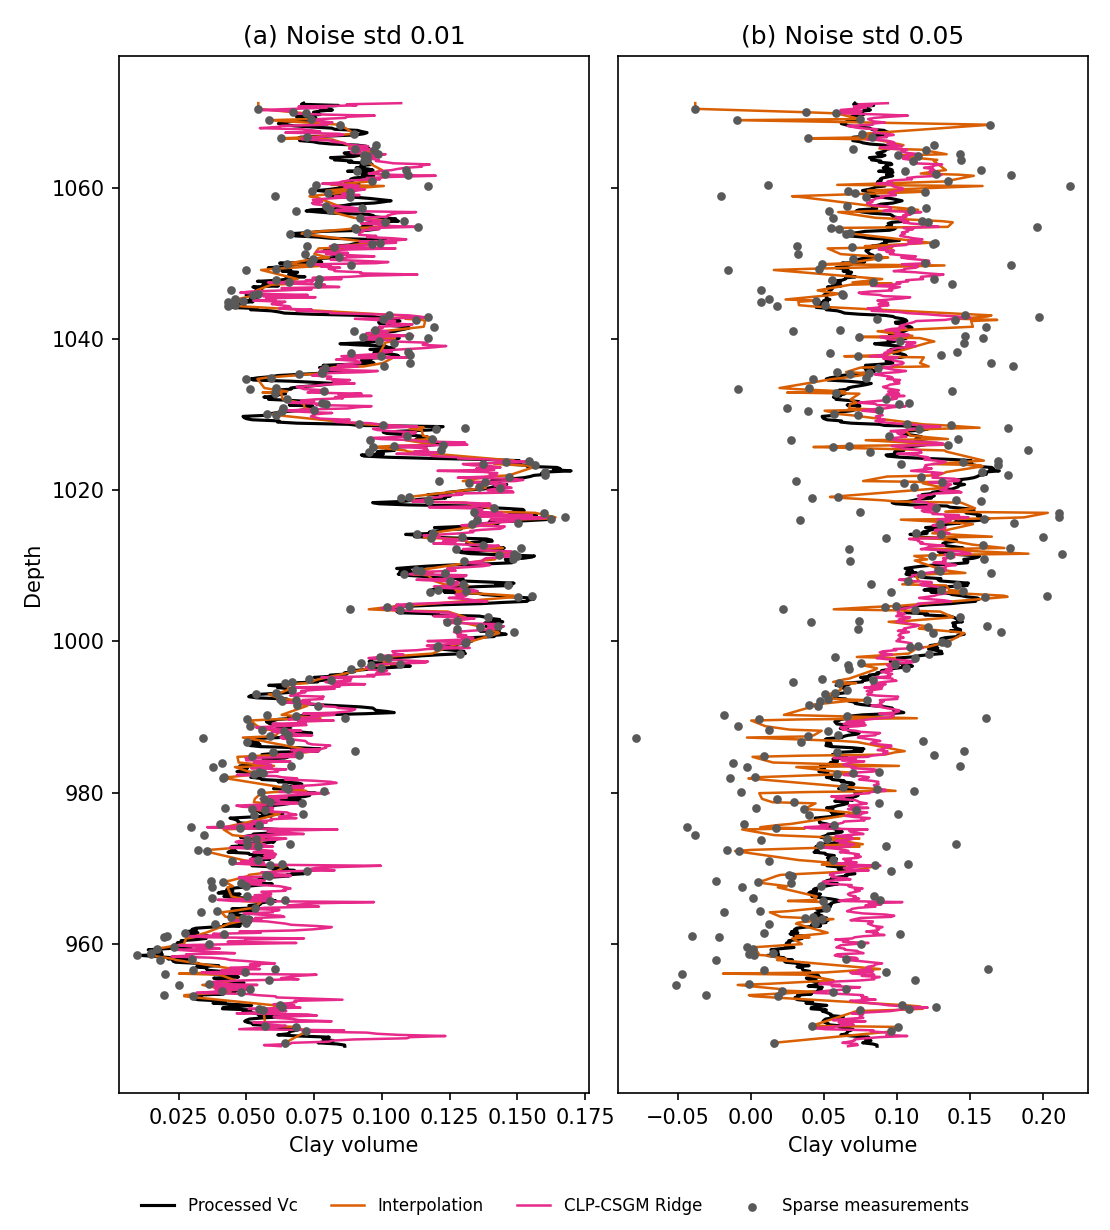
\includegraphics[width=\linewidth]{figures/crosswell_vc_noise_panels_step32_rho020_seed7.png}
  \caption{Held-out F03-4 depth tracks, seed $7$, step $32$, $\rho=0.20$.
  Panel (a) uses the published noise standard deviation $0.01$.
  Panel (b) uses $0.05$, the same order as the curve's standard deviation
  $0.035$. Each panel has its own clay-volume scale.
  This interval is one example. Tables~\ref{tab:crosswell_simple_baselines}
  and~\ref{tab:crosswell_noise_sweep} are the comparison.}
  \label{fig:crosswell_noise_panels}
\end{figure}

On the same splits, the retrospective decoder reconstruction
$G(E(\boldsymbol{y}))$ has mean test RMSE $0.0073$ at step $8$, $0.0099$ at
step $16$, and $0.0110$ at step $32$. That reconstruction is given the full
target window, so it is a check that the decoder can represent the curve. It
is not a predictor and it is not ranked with the methods above.

The step-$8$ pattern at noise standard deviation $0.05$ is compatible with
a limit of the dense-log map. It is not explained by the decoder check
alone, and these comparisons do not isolate that map as the only cause.
At step $8$ the decoder represents the held-out curve with mean test RMSE
$0.0073$. The window predicted from the dense logs alone has mean RMSE
$0.0564$. Interpolation at the same step and noise has mean RMSE $0.0456$
for $\rho=0.05$ and $0.0442$ for $\rho=0.10$. Those ratios observe $4$ and
$6$ coordinates in a window of length $64$. CLP-CSGM Ridge then stays
between the two, at $0.0508$ and $0.0456$. At $\rho=0.20$ the same window
observes $13$ coordinates, and CLP-CSGM Ridge has mean RMSE $0.0372$
against an interpolation RMSE of $0.0423$. At steps $16$ and $32$ the
dense-log window itself has mean RMSE $0.0426$ and $0.0432$, and
interpolation at this noise has errors of similar magnitude. Those similar
magnitudes do not show that the two reconstructions lie close to each
other. The pattern agrees with the ablation
in Section~\ref{subsec:ablation_analysis}, where the conditional code
$\boldsymbol{z}_0$ is not
helpful at step $8$.

\subsection{Wide-range depth profiles}
\label{app:crosswell_depth_wide}

Figure~\ref{fig:crosswell_depth_profile} omits MLP $[\boldsymbol{u},\boldsymbol{b}]$
and PCA $[\boldsymbol{u},\boldsymbol{b}]$ so that the reference, ML only, AE,
and CLP-CSGM Ridge can share one $V_c$ scale. Figure~\ref{fig:crosswell_depth_profile_wide}
uses the same held-out interval, step $16$, seed $7$, and $\rho=0.20$, and
shows every stored value of those two predictions. Their horizontal range
includes negative clay volume. No coordinate was dropped.

\begin{figure}[htbp]
  \centering
  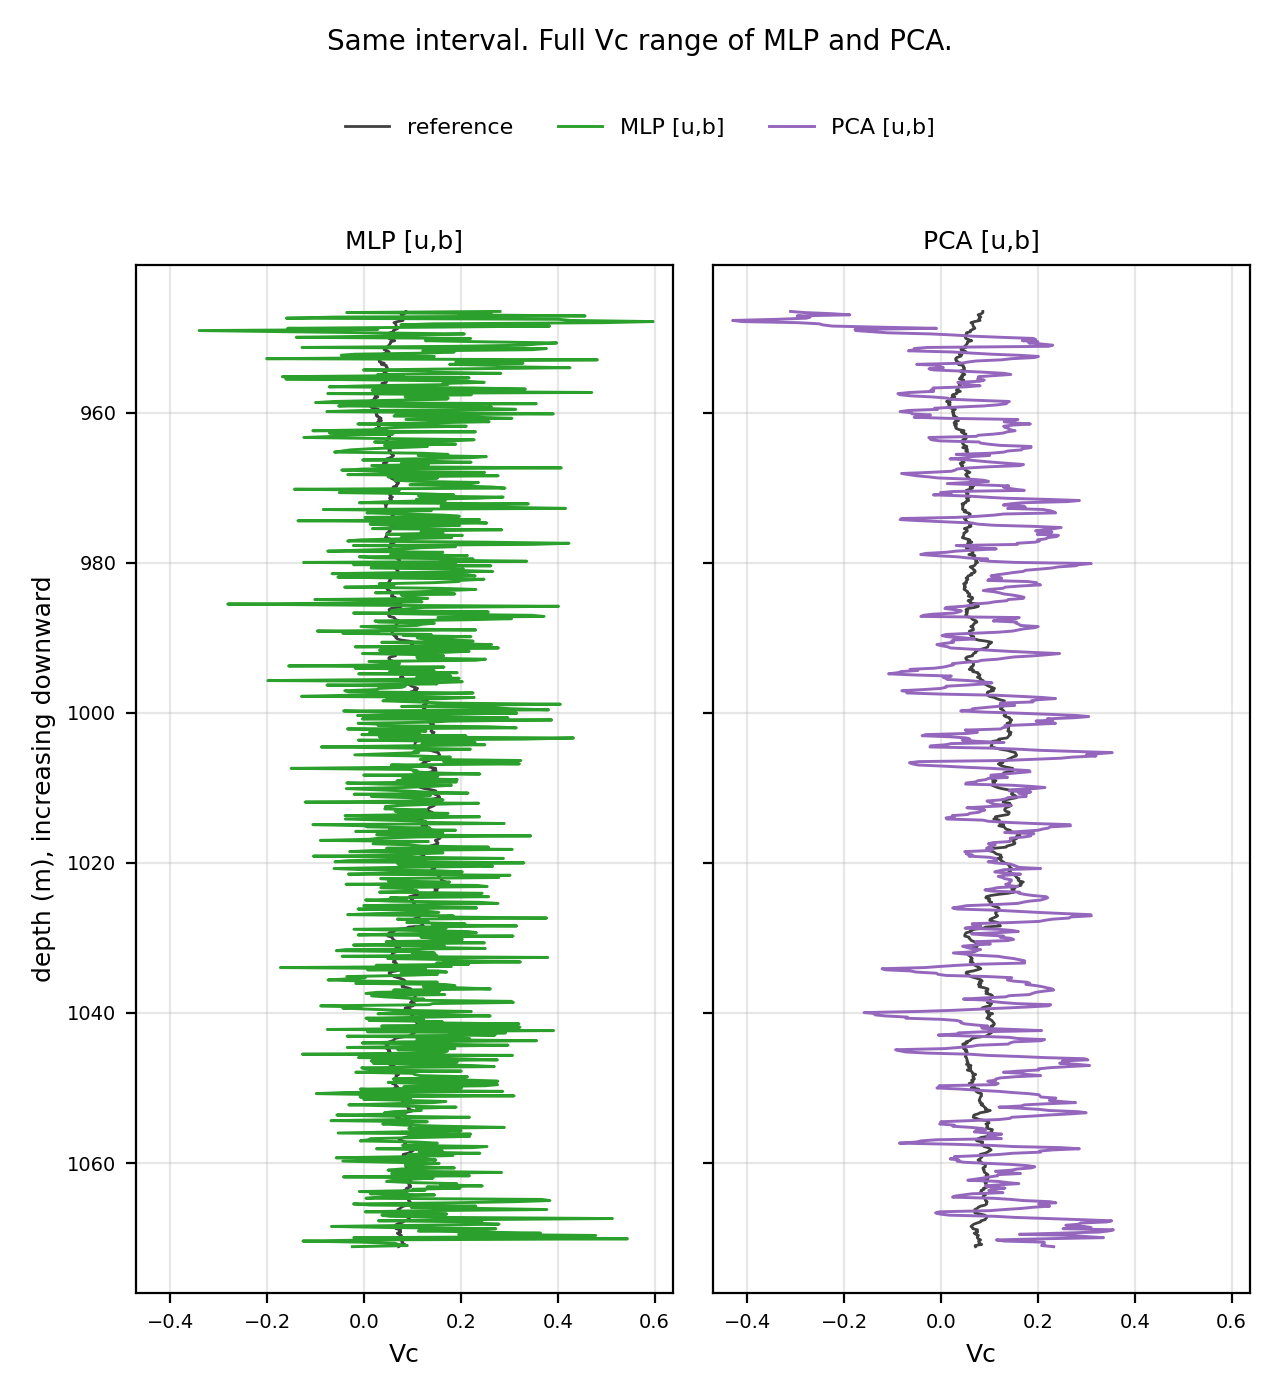
\includegraphics[width=0.92\linewidth]{10_depth_profile_crosswell_vc_wide.png}
  \caption{Same F03-4 interval as Fig.~\ref{fig:crosswell_depth_profile}.
  MLP $[\boldsymbol{u},\boldsymbol{b}]$ and PCA $[\boldsymbol{u},\boldsymbol{b}]$
  share the full horizontal range of their stored predictions. Depth
  increases downward.}
  \label{fig:crosswell_depth_profile_wide}
\end{figure}

\subsection{Computational Trade-Offs}
\label{app:runtime}

Table~\ref{tab:runtime_cost} and Fig.~\ref{fig:runtime_cost} quantify the
practical computational trade-off. CLP-CSGM
Ridge is more expensive than AE \([u,b]\) because it solves a latent inverse
problem at validation and test time instead of producing a single direct forward
prediction. Table~\ref{tab:runtime_cost} reports both mean wall-clock time per
test window and a separate normalized runtime diagnostic relative to AE; the
latter is the diagnostic shown in Fig.~\ref{fig:runtime_cost}; it is not the exact
quotient of the averaged seconds in the previous column. In the representative
cross-well case, the additional cost is substantial relative to AE, but CLP-CSGM
Ridge has the lowest mean RMSE among the methods listed in
Table~\ref{tab:runtime_cost}. That statement refers only to the computational-cost
table. It is not a ranking against the full set of comparators in the paper,
including depth interpolation. In the F03-4 GR-only case,
CLP-CSGM Ridge and AE \([u,b]\) have closer average RMSE, so the runtime gap is
less clearly justified. The extra optimization is most readily justified when
explicit sparse-measurement consistency produces a meaningful reconstruction
gain, especially under stronger ill-posedness or weaker direct supervision.

\begin{table}[htbp]
  \centering
  \caption{Representative computational-cost summary. Time is reported as average
  wall-clock seconds per test window across the tested measurement ratios. The
  normalized runtime diagnostic column is computed relative to AE \([u,b]\) within
  each dataset and should not be read as the exact quotient of the averaged
  wall-clock times.}
  \label{tab:runtime_cost}
  \resizebox{\linewidth}{!}{%
  \begin{tabular}{llccc}
    \toprule
    Dataset & Method & Time/window (s) & Normalized runtime diagnostic vs. AE & Mean RMSE \\
    \midrule
    Cross-well $V_c$ & ML only & 0.00787 & 0.32 & 0.02582 \\
    Cross-well $V_c$ & MLP \([u,b]\) & 0.04348 & 2.33 & 0.21399 \\
    Cross-well $V_c$ & PCA \([u,b]\) & 0.07129 & 3.15 & 0.14464 \\
    Cross-well $V_c$ & AE \([u,b]\) & 0.03156 & 1.00 & 0.01793 \\
    Cross-well $V_c$ & CLP-CSGM Ridge & 0.23517 & 9.79 & 0.01480 \\
    \midrule
    F03-4 GR-only & ML only & 0.06010 & 2.13 & 0.02391 \\
    F03-4 GR-only & MLP \([u,b]\) & 0.04771 & 1.73 & 0.03981 \\
    F03-4 GR-only & PCA \([u,b]\) & 0.31793 & 11.67 & 0.02149 \\
    F03-4 GR-only & AE \([u,b]\) & 0.02999 & 1.00 & 0.01429 \\
    F03-4 GR-only & CLP-CSGM Ridge & 0.08838 & 3.23 & 0.01418 \\
    \bottomrule
  \end{tabular}%
  }
\end{table}


\begin{figure}[htbp]
  \centering
  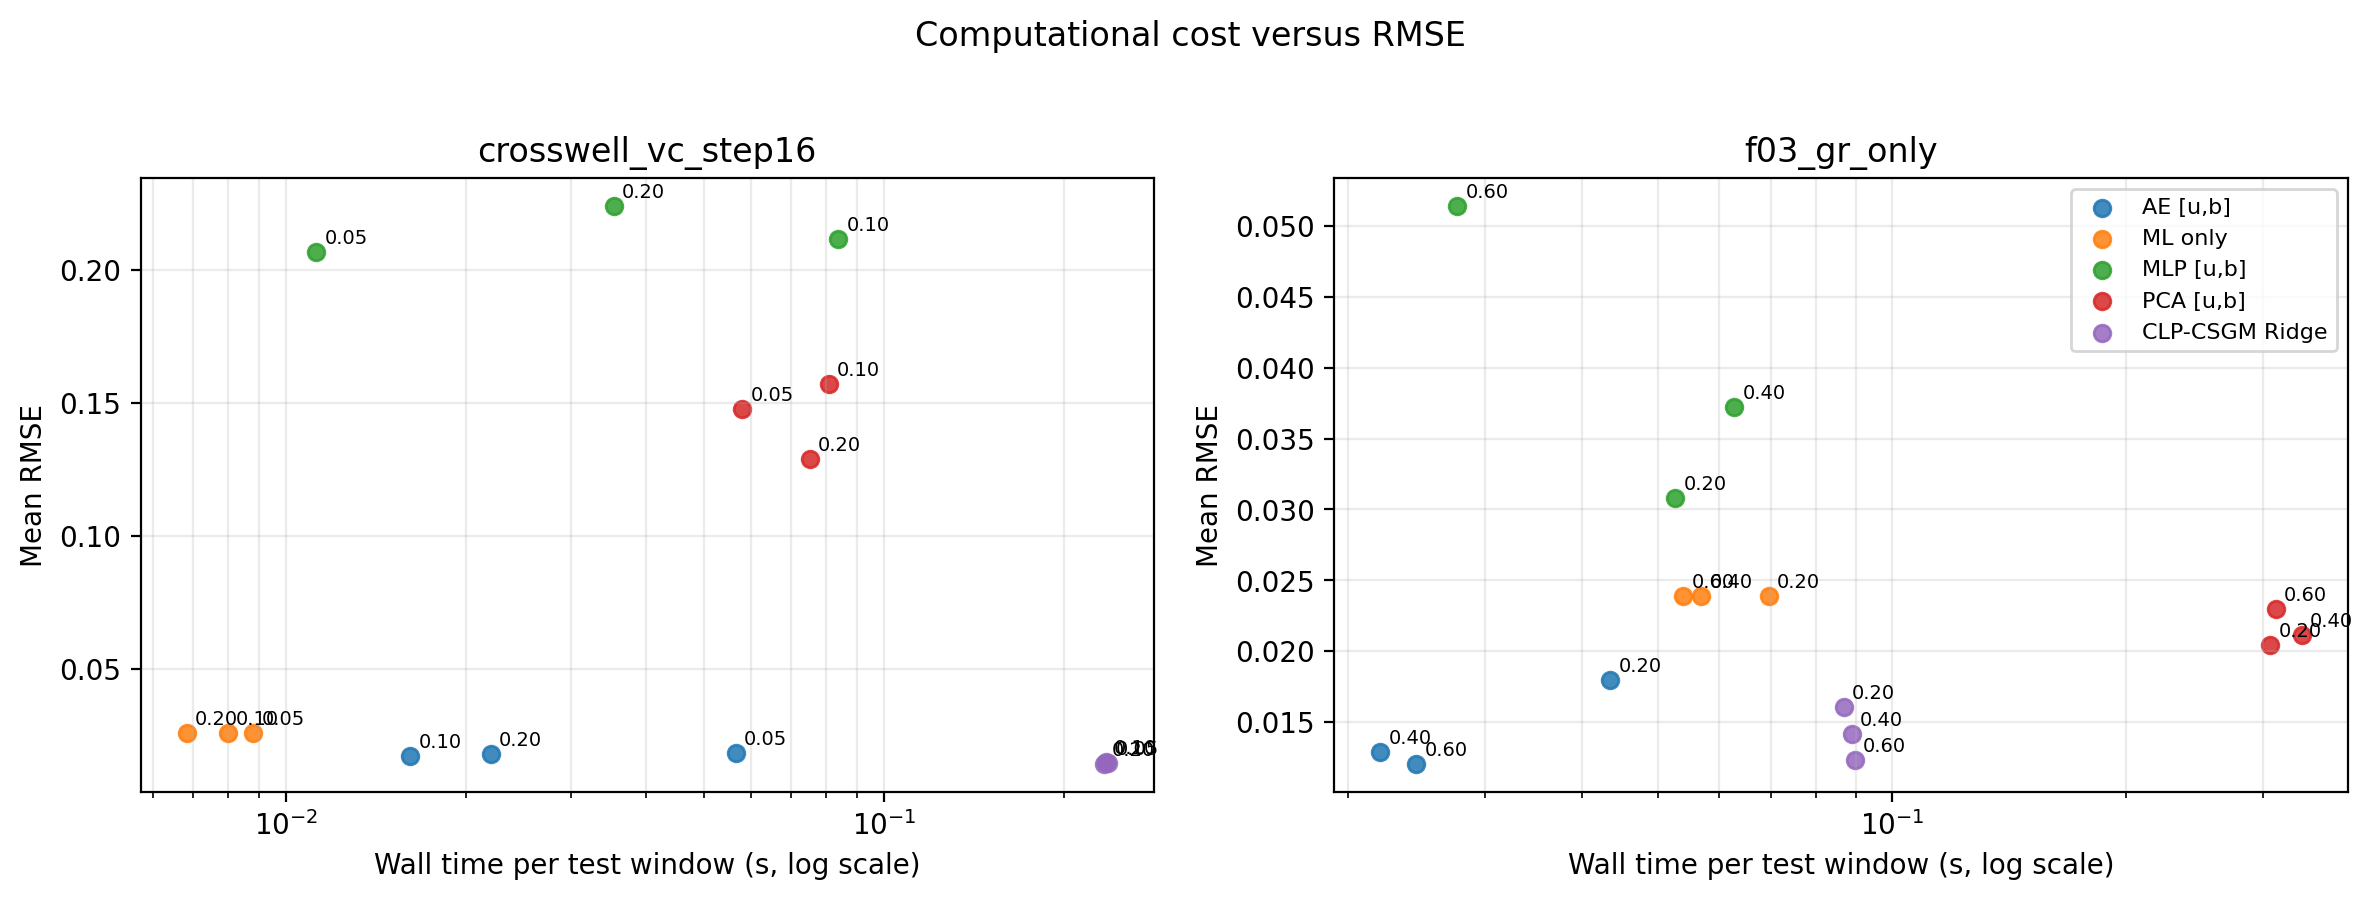
\includegraphics[width=\linewidth]{figures/runtime_vs_rmse.png}
  \vspace{0.5em}
  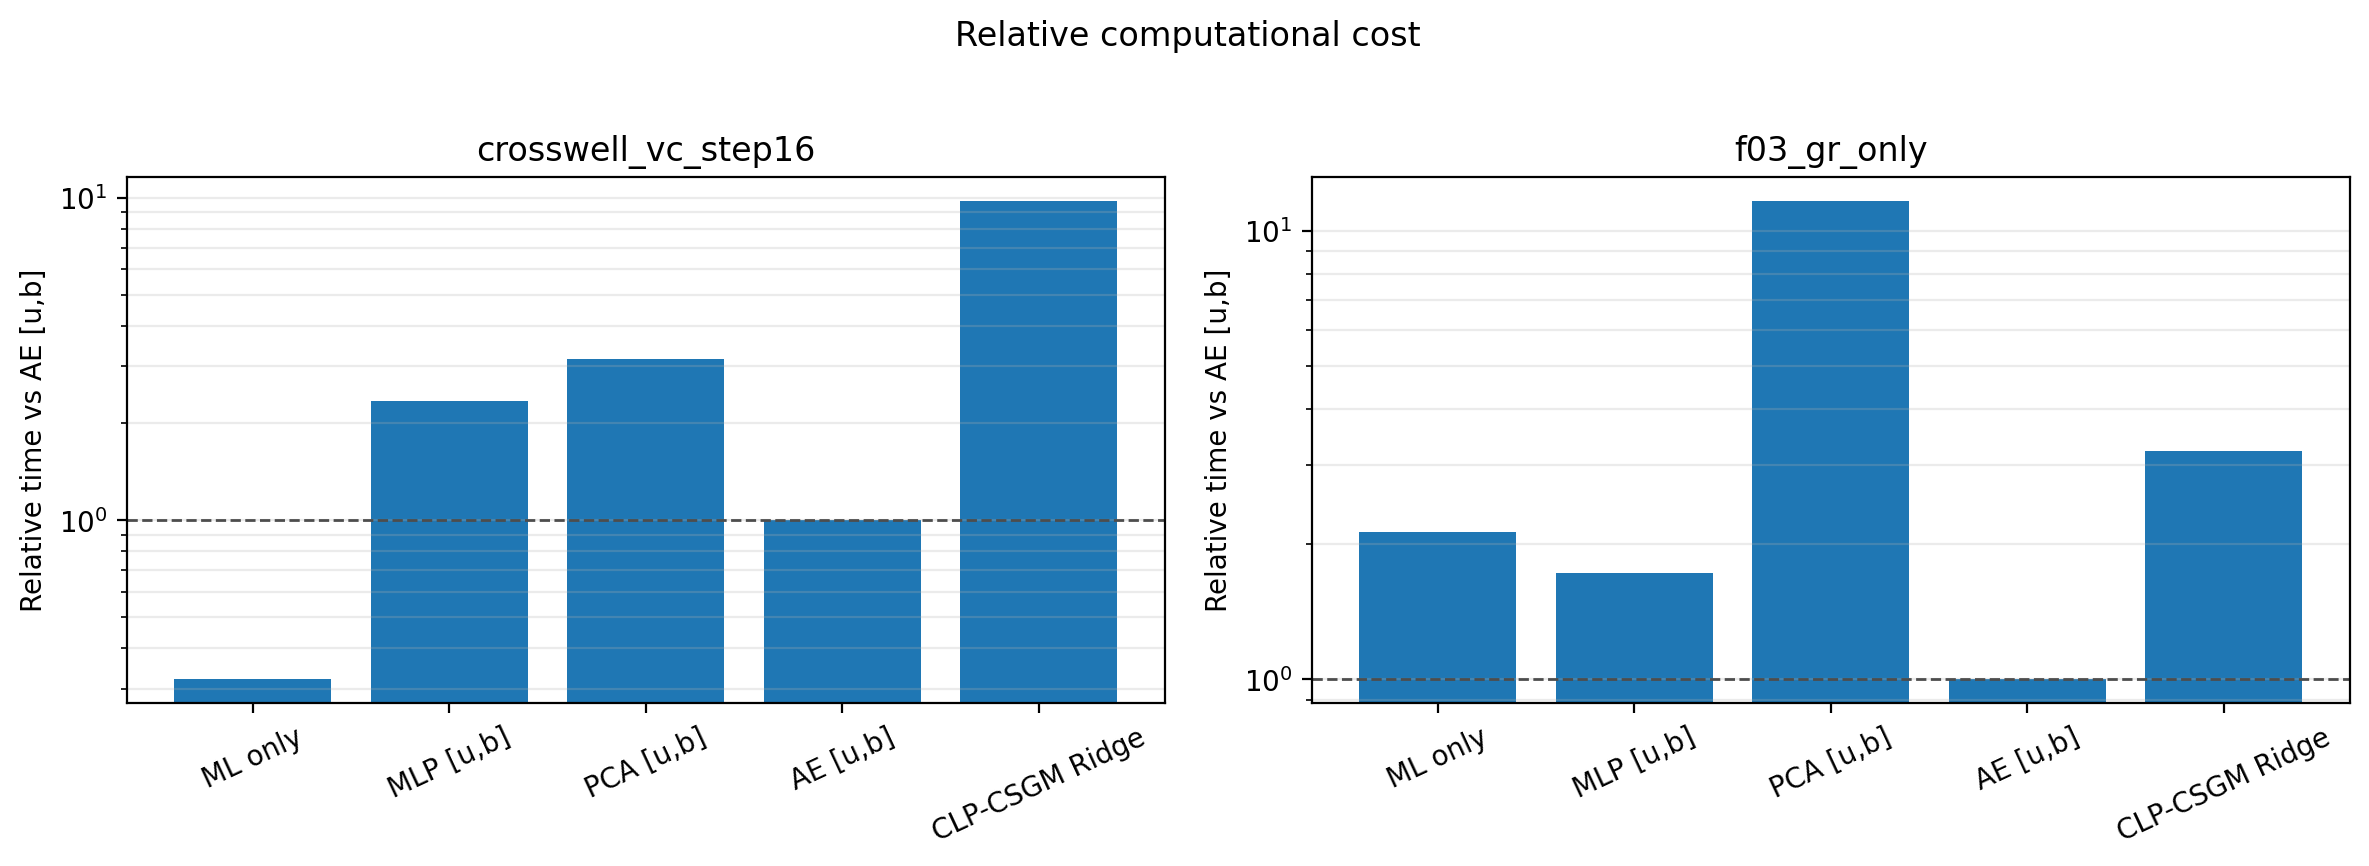
\includegraphics[width=\linewidth]{runtime_relative_vs_ae.png}
  \caption{Representative computational-cost diagnostics. The upper panel
  compares mean RMSE with wall-clock time per test window, and the lower panel
  reports the normalized runtime diagnostic relative to AE \([u,b]\) within
  each dataset.}
  \label{fig:runtime_cost}
\end{figure}

\section{Supplementary F03-4 GR-only stress tests}
\label{app:f03_stress}

The main F03-4 benchmark in Section~\ref{sec:results} uses
\(\rho\in\{0.20,0.30,\ldots,0.60\}\). This appendix summarizes controlled supplements on
the same well with GR-only \(u\), \(L{=}64\), depth-first splits before windowing,
coordinate subsampling, the same three fixed random-seed realizations, and the
same paired measurement protocol as Section~\ref{sec:experiments}. To align the
grid with the sparse end of the cross-well study, we use
\(\rho\in\{0.05,0.10,0.20\}\) and compare
CLP-CSGM Ridge with AE \([u,b]\).

Cases A--D differ only by the stress axes enumerated below:
\begin{itemize}
  \item \textbf{A (baseline noise):} \(\eta{=}0.01\) on \(b{=}My+\eta\); standard depth fractions \(0.6/0.2/0.2\); step \(1\).
  \item \textbf{B (noisy \(b\)):} \(\eta{=}0.05\); otherwise as A.
  \item \textbf{C (smaller train pool):} depth fractions \(0.45/0.25/0.30\); \(\eta{=}0.01\); step \(1\).
  \item \textbf{D (coarse sliding step):} step \(4\) with standard fractions;
  \(\eta{=}0.01\). This yields far fewer test windows
  (\(n_{\mathrm{test}}{=}56\) versus \(224\) in A/B), yielding high-variance
  paired RMSE summaries at each \(\rho\).
\end{itemize}

\begin{table}[htbp]
  \centering
  \caption{F03-4 GR-only stress tests: mean RMSE across seeds for AE \([u,b]\) versus CLP-CSGM Ridge.
  Relative RMSE gap is \((\mathrm{RMSE}_{\mathrm{AE}}-\mathrm{RMSE}_{\mathrm{Ridge}})/\mathrm{RMSE}_{\mathrm{AE}}\) in percent (positive favors Ridge).
  Test counts \(n_{\mathrm{test}}\) count windows in the test depth segment after sliding-window construction.}
  \label{tab:f03_stress}
  \small
  \adjustbox{max width=\linewidth}{\begin{tabular}{clcccc}
\toprule
Case & $\rho$ & AE \([u,b]\) & CLP-CSGM Ridge & Rel.\ RMSE gap (\%) & $n_{\mathrm{test}}$ \\
\midrule
A & 0.05 & 0.02011 & 0.01682 & +16.36 & 224 \\
 & 0.10 & 0.01900 & 0.01596 & +15.98 & 224 \\
 & 0.20 & 0.01489 & 0.01314 & +11.74 & 224 \\
\midrule
B & 0.05 & 0.02444 & 0.01919 & +21.51 & 224 \\
 & 0.10 & 0.02397 & 0.01897 & +20.87 & 224 \\
 & 0.20 & 0.02125 & 0.01846 & +13.13 & 224 \\
\midrule
C & 0.05 & 0.01810 & 0.01596 & +11.84 & 369 \\
 & 0.10 & 0.01712 & 0.01509 & +11.85 & 369 \\
 & 0.20 & 0.01433 & 0.01243 & +13.26 & 369 \\
\midrule
D & 0.05 & 0.01676 & 0.01672 & +0.24 & 56 \\
 & 0.10 & 0.01493 & 0.01547 & -3.62 & 56 \\
 & 0.20 & 0.01115 & 0.01298 & -16.33 & 56 \\
\bottomrule
\end{tabular}
}
\end{table}

In A--C, CLP-CSGM Ridge has lower mean RMSE than AE \([u,b]\) at every tested
\(\rho\), including under larger \(\eta\) and smaller training fractions. In D,
mean RMSE crosses over at \(\rho\in\{0.10,0.20\}\) and is similar to or slightly
lower at \(\rho{=}0.05\). The small effective test count is consistent with this
behavior because aggressive overlap reduction amplifies seed variability.
The A--D results position the coarse-step F03 stress as an exploratory supplement
to the primary \(\rho\) sweep in Table~\ref{tab:f03_results}.

\section{Supplementary Lapa Pre-salt Permeability Case Study}
\label{app:lapa_case}

This appendix reports a complementary case study built from the well-log and
permeability data context described by \citet{alvarez2025nonlinear} for the
Lapa pre-salt carbonate reservoir in the Santos Basin. Geologically, the Lapa
oilfield targets the Aptian Barra Velha Formation, a heterogeneous pre-salt
carbonate succession in which laminated microbialites, spherulite,
stromatolite, rudstone, and grainstone facies coexist. In such rocks,
permeability is controlled by pore structure and diagenesis as much as by
porosity. Permeability is therefore the sparse reconstruction target in this
supplementary check. Full core--log integration,
hydraulic flow units, and nonlinear permeability prediction details are
reported in \citet{alvarez2025nonlinear}. The benchmark adaptation uses
the same CLP-CSGM protocol as the main paper: sliding
windows, contiguous train/validation/test split, coordinate subsampling for
sparse target observations, paired seeds and measurement ratios, and matched
direct \([u,b]\) baselines.

This limited-sample case provides supplementary evidence. The configuration uses
\(L=16\), step
\(=4\), seven dense channels in \(u\), target \(k_{\mathrm{lab}}\) in
\(\log_{10}\) scale,
\(\rho\in\{0.20,0.30,0.40,0.50,0.60\}\), and the same three fixed random-seed
realizations used only for reproducible paired averaging.

\begin{table}[htbp]
  \centering
  \caption{Supplementary Lapa case study by measurement ratio. Values are
  means over three seeds.}
  \label{tab:lapa_results}
  \small
  \adjustbox{max width=\linewidth}{\begin{tabular}{rlrrr}
\toprule
rho & method & rmse & mae & relative\_l2 \\
\midrule
0.20000 & CLP-CSGM MLP & 1.07615 & 0.84823 & 1.00530 \\
0.20000 & CLP-CSGM Ridge & 1.22639 & 0.97273 & 1.08660 \\
0.20000 & Measurement-only CSGM & 1.03628 & 0.75013 & 0.93124 \\
0.20000 & AE [u,b] & 1.30639 & 1.11253 & 1.22956 \\
0.20000 & PCA [u,b] & 1.73942 & 1.42881 & 1.60571 \\
0.20000 & ML only & 2.06280 & 1.70838 & 2.00587 \\
0.20000 & MLP [u,b] & 2.21106 & 1.78860 & 2.13801 \\
0.30000 & CLP-CSGM MLP & 1.07099 & 0.81987 & 0.96733 \\
0.30000 & CLP-CSGM Ridge & 1.06503 & 0.79065 & 0.91318 \\
0.30000 & Measurement-only CSGM & 0.96152 & 0.67917 & 0.86494 \\
0.30000 & AE [u,b] & 1.39133 & 1.17212 & 1.30771 \\
0.30000 & PCA [u,b] & 1.89848 & 1.57954 & 1.72206 \\
0.30000 & ML only & 2.06280 & 1.70838 & 2.00587 \\
0.30000 & MLP [u,b] & 2.14391 & 1.73034 & 2.00236 \\
0.40000 & CLP-CSGM MLP & 0.96555 & 0.73670 & 0.88465 \\
0.40000 & CLP-CSGM Ridge & 0.97383 & 0.71050 & 0.86519 \\
0.40000 & Measurement-only CSGM & 0.97680 & 0.65052 & 0.86968 \\
0.40000 & AE [u,b] & 1.44311 & 1.21575 & 1.35981 \\
0.40000 & PCA [u,b] & 1.87246 & 1.54857 & 1.79426 \\
0.40000 & ML only & 2.06280 & 1.70838 & 2.00587 \\
0.40000 & MLP [u,b] & 2.27913 & 1.85405 & 2.18847 \\
0.50000 & CLP-CSGM MLP & 0.95447 & 0.74089 & 0.84011 \\
0.50000 & CLP-CSGM Ridge & 0.99413 & 0.75851 & 0.85865 \\
0.50000 & Measurement-only CSGM & 0.91277 & 0.55221 & 0.80389 \\
0.50000 & AE [u,b] & 1.36684 & 1.18683 & 1.24828 \\
0.50000 & PCA [u,b] & 2.03242 & 1.68385 & 1.85003 \\
0.50000 & ML only & 2.06280 & 1.70838 & 2.00587 \\
0.50000 & MLP [u,b] & 2.05267 & 1.61547 & 2.03388 \\
0.60000 & CLP-CSGM MLP & 0.78164 & 0.59283 & 0.70811 \\
0.60000 & CLP-CSGM Ridge & 0.74144 & 0.54218 & 0.67252 \\
0.60000 & Measurement-only CSGM & 0.84417 & 0.45574 & 0.74392 \\
0.60000 & AE [u,b] & 1.31942 & 1.11830 & 1.22740 \\
0.60000 & PCA [u,b] & 1.88084 & 1.56736 & 1.77341 \\
0.60000 & ML only & 2.06280 & 1.70838 & 2.00587 \\
0.60000 & MLP [u,b] & 2.27679 & 1.86123 & 2.16631 \\
\bottomrule
\end{tabular}
}
\end{table}

Table~\ref{tab:lapa_results} shows that both CLP-CSGM prior variants remain
competitive with direct \([u,b]\) baselines across the tested \(\rho\) grid.
CLP-CSGM MLP and CLP-CSGM Ridge have lower mean RMSE than AE \([u,b]\), PCA
\([u,b]\), ML only, and direct MLP \([u,b]\) at all reported ratios. The comparison with
measurement-only CSGM is ratio-dependent: measurement-only has lower mean RMSE
at some lower or intermediate ratios, while the prior-guided variants have
lower mean RMSE at others. This variation is consistent with the expected
regime dependence when sparse measurements are informative but the sample size
is limited.

\begin{figure}[htbp]
  \centering
  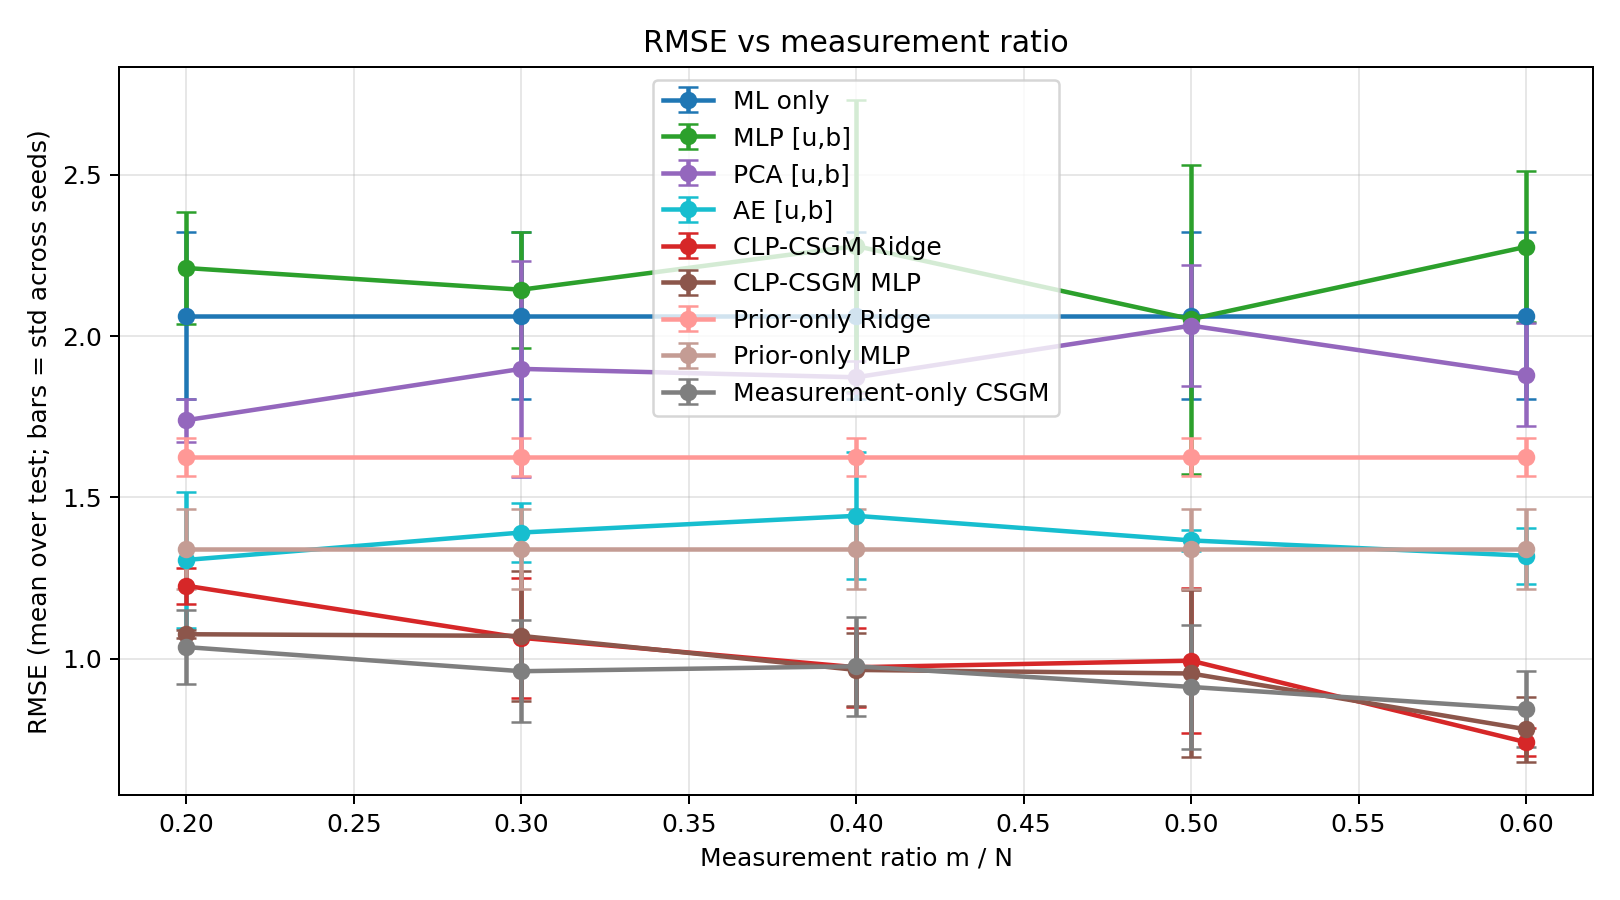
\includegraphics[width=0.92\linewidth]{figures/lapa_01_rmse_vs_measurement_ratio.png}
  \caption{Supplementary Lapa case study RMSE by measurement ratio. Prior-guided
  CLP-CSGM variants remain competitive across the sparse-measurement grid.}
  \label{fig:lapa_rmse}
\end{figure}

\begin{figure}[htbp]
  \centering
  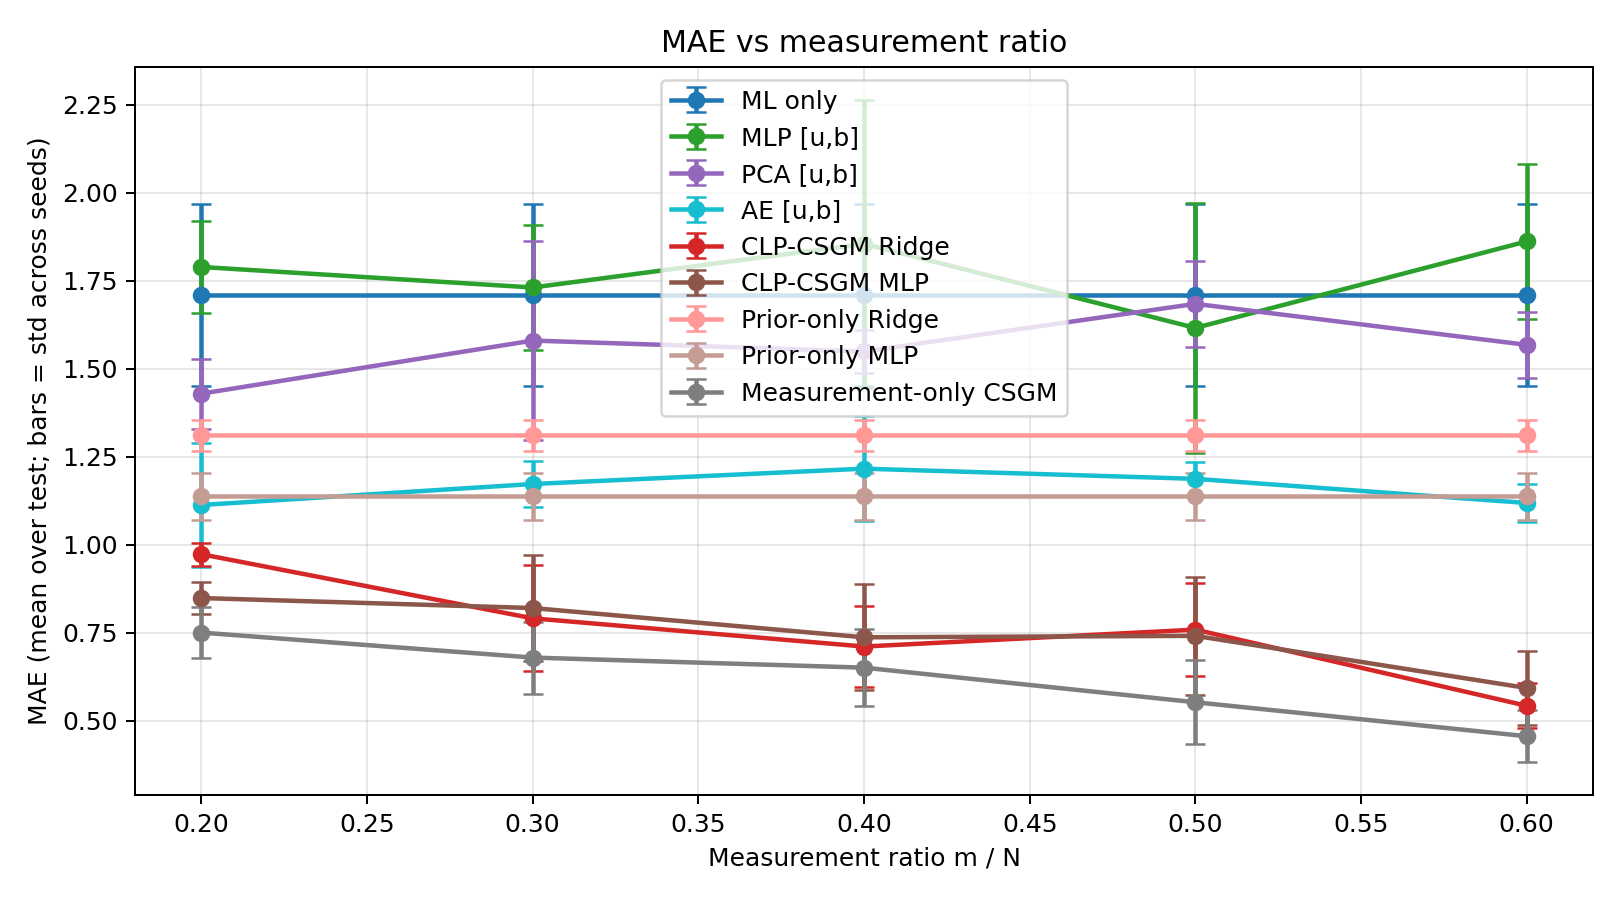
\includegraphics[width=0.92\linewidth]{figures/lapa_02_mae_vs_measurement_ratio.png}
  \caption{Supplementary Lapa case study MAE by measurement ratio. The ranking
  pattern is consistent with the RMSE view.}
  \label{fig:lapa_mae}
\end{figure}

\begin{figure}[htbp]
  \centering
  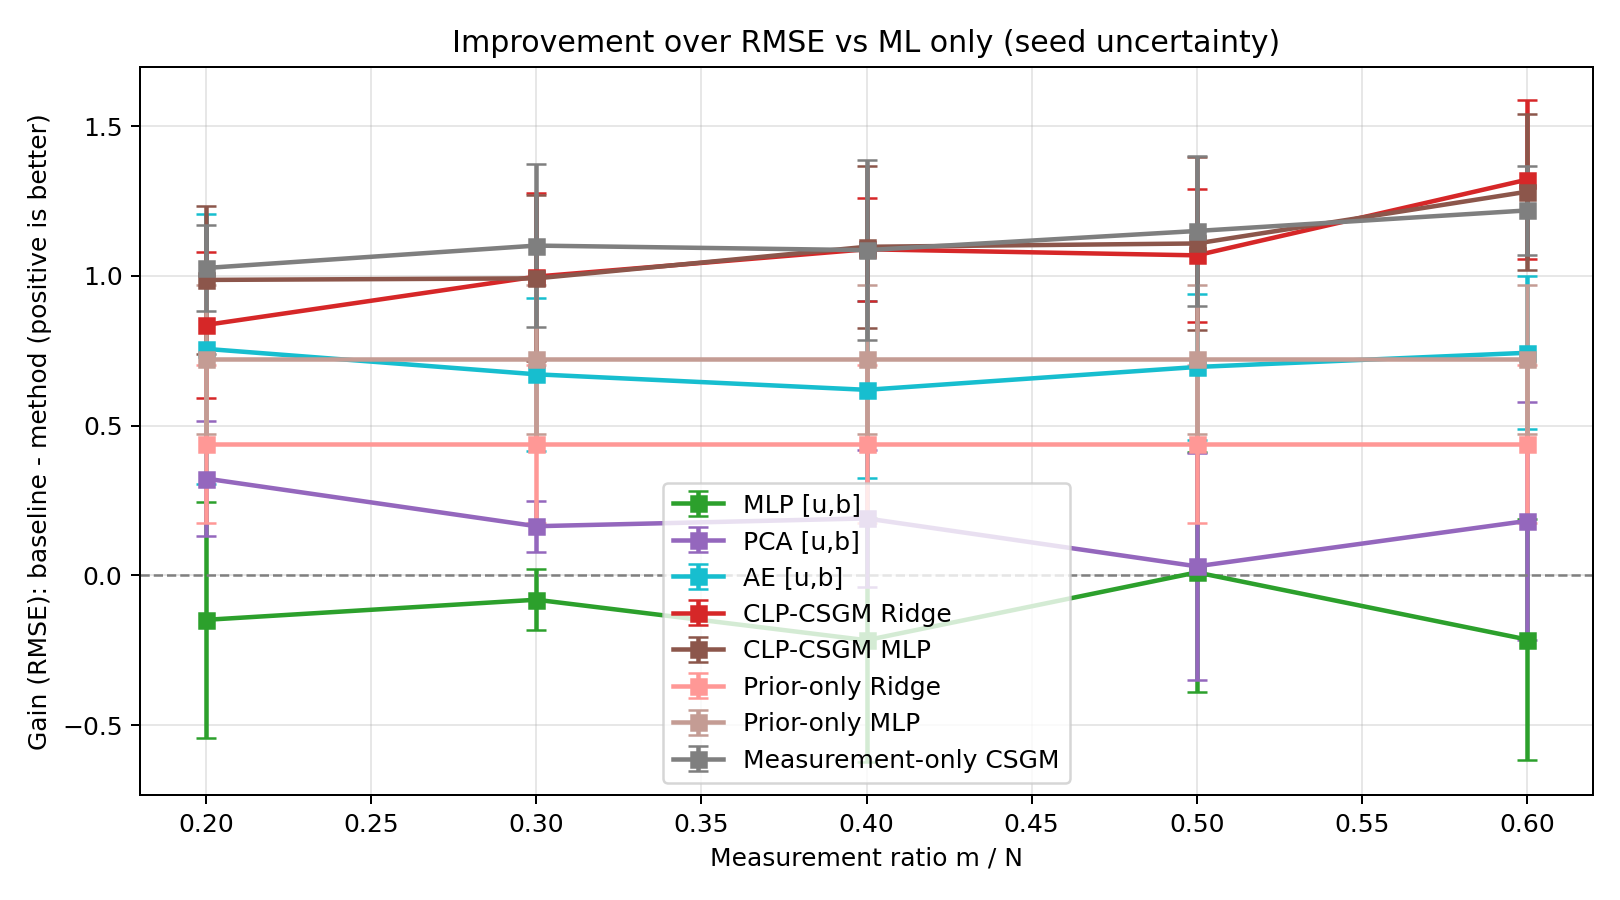
\includegraphics[width=0.92\linewidth]{figures/lapa_06_gain_rmse_over_ml_only.png}
  \caption{Supplementary Lapa case study RMSE gain over ML-only. Positive values
  indicate improvement over dense-context-only prediction.}
  \label{fig:lapa_gain}
\end{figure}

\begin{figure}[htbp]
  \centering
  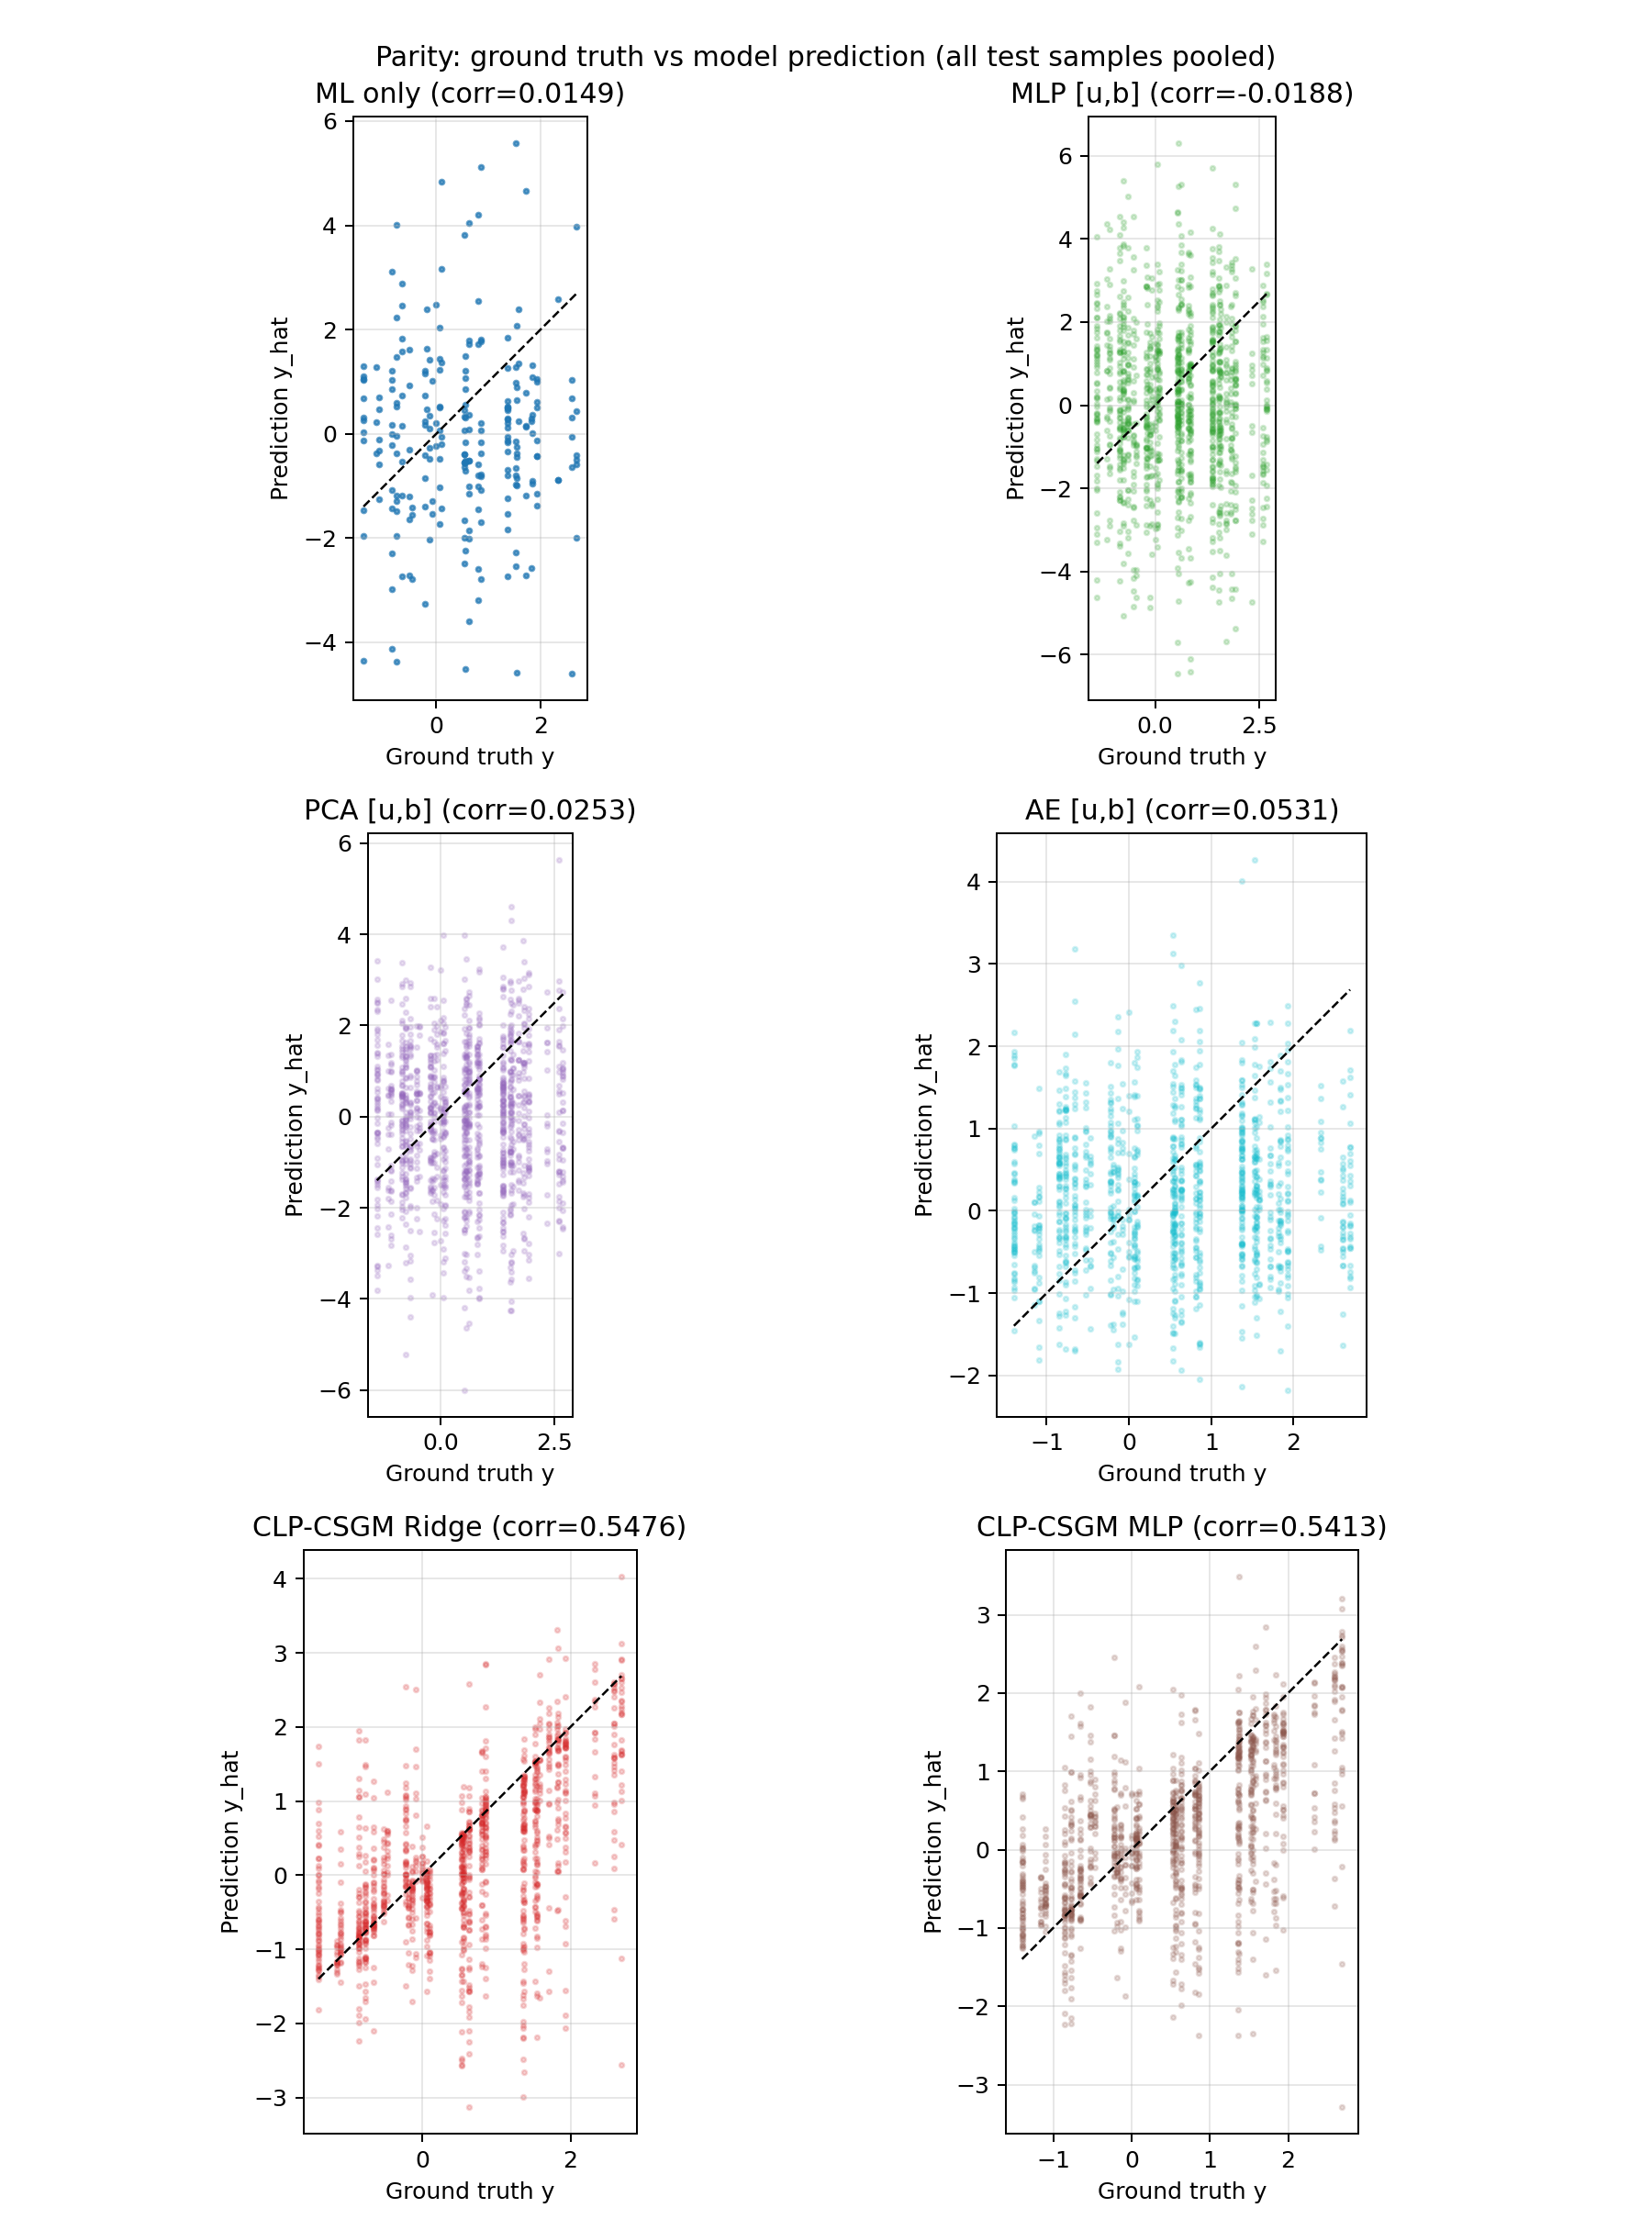
\includegraphics[width=0.82\linewidth]{figures/lapa_09_parity_ground_truth_vs_prediction.png}
  \caption{Supplementary Lapa pooled parity plot. The visual agreement is consistent with the
  quantitative summary, while still reflecting variability expected under small
  test counts.}
  \label{fig:lapa_parity}
\end{figure}

\section{Laboratory porosity on a cored interval}
\label{app:phi_lab_861}

This supplement uses the 87 laboratory-porosity samples of well 861 over
$5205.91$--$5233.72~\mathrm{m}$. The target consists of porosity values
identified as laboratory measurements in the Auddys source dataset
($\mathrm{Logs}$ table). These values are not deterministically computed from
the auxiliary gamma-ray, resistivity, or lithotype channels by our processing
pipeline. Original per-plug laboratory assay records were not available for
independent verification. Dense context is gamma ray, deep resistivity,
shallow resistivity, and lithotype. Density, neutron porosity, sonic porosity,
and $\mathrm{Phi_{ND}}$ are excluded because they track $\mathrm{Phi_{lab}}$.

Training and test samples are separated into contiguous depth blocks before
window construction. Windows have length $8$ and step $1$. The last $16$ rows
of the deepest training block form the validation segment. Seeds are
$\{7,23,41\}$. For each fold, seed, and ratio, one coordinate set is shared by
every window. The laboratory value on those coordinates is the measurement,
with no added noise. Within each test window, RMSE is computed only at
coordinates not supplied as measurements to that particular reconstruction.
However, because the length-$8$ windows overlap with step $1$, the same
physical depth can be measured in one window and scored as unobserved in
another. This protocol evaluates within-window sparse assimilation on
depth-held-out test blocks, not reconstruction at physical depths withheld
globally from all test windows. Across the $18$ fold--seed--ratio
configurations, $21$--$27$ physical depths per test block appear both as
measured and scored coordinates across different windows. Between $84\%$ and
$100\%$ of scored residual entries correspond to physical depths that were
supplied as measurements in at least one other window. Those percentages count
residual entries, not RMSE contribution, and they do not indicate training
leakage: training and test rows remain disjoint. The nine results per ratio
are three depth blocks repeated under three seeds, not nine independent
geological intervals. $\rho=0.25$ uses $m=2$ measurements and $\rho=0.50$ uses
$m=4$. Coordinate sets are sampled separately at each ratio. The direct AE
receives $[\boldsymbol{u},\boldsymbol{b}]$ with the same coordinates.
The decoded prediction of the conditional prior is
$G(h(\boldsymbol{u}))$, with no latent search. It is reported below as the
log-only anchor. Neither
method is added to the main F3 tables.

\begin{table}[htbp]
  \centering
  \caption{Well 861 laboratory-porosity supplement. Entries are the mean
  within-window held-out RMSE across three depth blocks and three seeds
  ($n=9$ block--seed pairs, not nine independent intervals). $\Delta$ is
  AE minus CLP-CSGM Ridge; a negative value means the direct AE has the lower
  mean. CLP$>$AE counts splits in which CLP-CSGM Ridge has the lower RMSE.}
  \label{tab:phi_lab_861}
  \small
  \adjustbox{max width=\linewidth}{\begin{tabular}{rrrrrr}
\toprule
$\rho$ & CLP & AE $[u,b]$ & prior-only & $\Delta$ AE & CLP$>$AE \\
\midrule
0.25 & 0.0602 & 0.0537 & 0.0729 & -0.0065 & 5/9 \\
0.50 & 0.0580 & 0.0523 & 0.0753 & -0.0057 & 6/9 \\
\bottomrule
\end{tabular}
}
\end{table}

Table~\ref{tab:phi_lab_861} shows that the direct AE has the lower mean
held-out RMSE at both ratios. CLP-CSGM Ridge has the lower RMSE in five of
nine splits at $\rho=0.25$ and in six of nine at $\rho=0.50$, and it has lower
RMSE than the log-only anchor in all nine splits at both ratios. The two
summaries answer different questions. The mean asks which method is lower
after every split is weighted equally. The split count asks how often
CLP-CSGM Ridge is the lower of the two. They disagree because one depth block
carries errors large enough to set the mean.

\begin{table}[htbp]
  \centering
  \caption{Well 861 held-out laboratory-porosity RMSE by depth block. Each
  entry is the mean across the three seeds. Prior-only is $G(h(\boldsymbol{u}))$
  with no measurement term.}
  \label{tab:phi_lab_861_blocks}
  \small
  \adjustbox{max width=\linewidth}{\begin{tabular}{llrrrr}
\toprule
Block & $\rho$ & CLP & AE $[u,b]$ & prior-only \\
\midrule
5205.91--5214.48 m & 0.25 & 0.0338 & 0.0371 & 0.0486 \\
5205.91--5214.48 m & 0.50 & 0.0228 & 0.0350 & 0.0472 \\
5214.67--5223.63 m & 0.25 & 0.0536 & 0.0548 & 0.0559 \\
5214.67--5223.63 m & 0.50 & 0.0497 & 0.0543 & 0.0554 \\
5224.39--5233.72 m & 0.25 & 0.0931 & 0.0691 & 0.1142 \\
5224.39--5233.72 m & 0.50 & 0.1016 & 0.0676 & 0.1234 \\
\bottomrule
\end{tabular}
}
\end{table}

Table~\ref{tab:phi_lab_861_blocks} locates the block-level pattern. On
$5205.91$--$5214.48~\mathrm{m}$, CLP-CSGM Ridge has the lower block-mean RMSE
at both ratios. In the shallowest block, mean held-out RMSE decreases from
$0.0338$ at $\rho=0.25$ to $0.0228$ at $\rho=0.50$, while the direct AE stays
near $0.035$. Because the coordinate sets are sampled separately at each
measurement ratio, this comparison changes both the number and the placement
of observations and does not isolate the effect of measurement count. On
$5214.67$--$5223.63~\mathrm{m}$ the two methods are close, with CLP-CSGM Ridge
still slightly lower. On $5224.39$--$5233.72~\mathrm{m}$ the direct AE is lower
by a wide margin ($0.0691$ and $0.0676$ against $0.0931$ and $0.1016$).

In every block and at both ratios, CLP-CSGM Ridge has lower RMSE than the
log-only anchor $G(h(\boldsymbol{u}))$. In the shallowest block, mean
$\mathrm{Phi_{lab}}$ is $0.092$ with standard deviation $0.019$, mean gamma ray
is about $15~\mathrm{API}$, and the median deep resistivity is about $1900$.
The direct AE already receives the laboratory coordinates as input features.
Each test fold still has $28$ to $35$ overlapping training windows, so this is
not the scarce-window regime of the F3 steps $16$ and $32$.

The larger share of the pooled AE advantage sits in the deepest block. When
that block is held out, mean $\mathrm{Phi_{lab}}$ rises to $0.145$, mean gamma
ray rises to about $30~\mathrm{API}$, and the median deep resistivity falls to
about $600$. The lithotype mix also changes: codes $2$ and $4$ account for
$25$ of the $29$ rows, whereas the middle block is mostly code $1$. The
decoded prediction $G(\boldsymbol{z}_0)$ differs substantially from the target
windows there. With only $m=2$ or $m=4$ measurements in a length-$8$ window,
CLP-CSGM Ridge still improves on that anchor ($0.0931$ versus $0.1142$, and
$0.1016$ versus $0.1234$) but does not catch the direct AE.

The results are consistent with the hypothesis that sparse-measurement
refinement is more effective when the conditional latent prior provides a
representation compatible with the target interval. The larger errors in the
deepest block coincide with changes in the auxiliary-log characteristics and a
less accurate prior-only reconstruction. However, the present experiment does
not isolate prior mismatch as the causal factor explaining the relative
performance of CLP-CSGM and the direct autoencoder. The result does not extend
the F3 low-support advantage to a mean win on this laboratory target. It is
one cored interval.